% Options for packages loaded elsewhere
\PassOptionsToPackage{unicode}{hyperref}
\PassOptionsToPackage{hyphens}{url}
%
\documentclass[
]{article}
\title{ACLIM2 CMIP6 ROMSNPZ Indices quick start guide}
\author{K. Holsman}
\date{}

\usepackage{amsmath,amssymb}
\usepackage{lmodern}
\usepackage{iftex}
\ifPDFTeX
  \usepackage[T1]{fontenc}
  \usepackage[utf8]{inputenc}
  \usepackage{textcomp} % provide euro and other symbols
\else % if luatex or xetex
  \usepackage{unicode-math}
  \defaultfontfeatures{Scale=MatchLowercase}
  \defaultfontfeatures[\rmfamily]{Ligatures=TeX,Scale=1}
\fi
% Use upquote if available, for straight quotes in verbatim environments
\IfFileExists{upquote.sty}{\usepackage{upquote}}{}
\IfFileExists{microtype.sty}{% use microtype if available
  \usepackage[]{microtype}
  \UseMicrotypeSet[protrusion]{basicmath} % disable protrusion for tt fonts
}{}
\makeatletter
\@ifundefined{KOMAClassName}{% if non-KOMA class
  \IfFileExists{parskip.sty}{%
    \usepackage{parskip}
  }{% else
    \setlength{\parindent}{0pt}
    \setlength{\parskip}{6pt plus 2pt minus 1pt}}
}{% if KOMA class
  \KOMAoptions{parskip=half}}
\makeatother
\usepackage{xcolor}
\IfFileExists{xurl.sty}{\usepackage{xurl}}{} % add URL line breaks if available
\IfFileExists{bookmark.sty}{\usepackage{bookmark}}{\usepackage{hyperref}}
\hypersetup{
  pdftitle={ACLIM2 CMIP6 ROMSNPZ Indices quick start guide},
  pdfauthor={K. Holsman},
  hidelinks,
  pdfcreator={LaTeX via pandoc}}
\urlstyle{same} % disable monospaced font for URLs
\usepackage[margin=1in]{geometry}
\usepackage{color}
\usepackage{fancyvrb}
\newcommand{\VerbBar}{|}
\newcommand{\VERB}{\Verb[commandchars=\\\{\}]}
\DefineVerbatimEnvironment{Highlighting}{Verbatim}{commandchars=\\\{\}}
% Add ',fontsize=\small' for more characters per line
\usepackage{framed}
\definecolor{shadecolor}{RGB}{248,248,248}
\newenvironment{Shaded}{\begin{snugshade}}{\end{snugshade}}
\newcommand{\AlertTok}[1]{\textcolor[rgb]{0.94,0.16,0.16}{#1}}
\newcommand{\AnnotationTok}[1]{\textcolor[rgb]{0.56,0.35,0.01}{\textbf{\textit{#1}}}}
\newcommand{\AttributeTok}[1]{\textcolor[rgb]{0.77,0.63,0.00}{#1}}
\newcommand{\BaseNTok}[1]{\textcolor[rgb]{0.00,0.00,0.81}{#1}}
\newcommand{\BuiltInTok}[1]{#1}
\newcommand{\CharTok}[1]{\textcolor[rgb]{0.31,0.60,0.02}{#1}}
\newcommand{\CommentTok}[1]{\textcolor[rgb]{0.56,0.35,0.01}{\textit{#1}}}
\newcommand{\CommentVarTok}[1]{\textcolor[rgb]{0.56,0.35,0.01}{\textbf{\textit{#1}}}}
\newcommand{\ConstantTok}[1]{\textcolor[rgb]{0.00,0.00,0.00}{#1}}
\newcommand{\ControlFlowTok}[1]{\textcolor[rgb]{0.13,0.29,0.53}{\textbf{#1}}}
\newcommand{\DataTypeTok}[1]{\textcolor[rgb]{0.13,0.29,0.53}{#1}}
\newcommand{\DecValTok}[1]{\textcolor[rgb]{0.00,0.00,0.81}{#1}}
\newcommand{\DocumentationTok}[1]{\textcolor[rgb]{0.56,0.35,0.01}{\textbf{\textit{#1}}}}
\newcommand{\ErrorTok}[1]{\textcolor[rgb]{0.64,0.00,0.00}{\textbf{#1}}}
\newcommand{\ExtensionTok}[1]{#1}
\newcommand{\FloatTok}[1]{\textcolor[rgb]{0.00,0.00,0.81}{#1}}
\newcommand{\FunctionTok}[1]{\textcolor[rgb]{0.00,0.00,0.00}{#1}}
\newcommand{\ImportTok}[1]{#1}
\newcommand{\InformationTok}[1]{\textcolor[rgb]{0.56,0.35,0.01}{\textbf{\textit{#1}}}}
\newcommand{\KeywordTok}[1]{\textcolor[rgb]{0.13,0.29,0.53}{\textbf{#1}}}
\newcommand{\NormalTok}[1]{#1}
\newcommand{\OperatorTok}[1]{\textcolor[rgb]{0.81,0.36,0.00}{\textbf{#1}}}
\newcommand{\OtherTok}[1]{\textcolor[rgb]{0.56,0.35,0.01}{#1}}
\newcommand{\PreprocessorTok}[1]{\textcolor[rgb]{0.56,0.35,0.01}{\textit{#1}}}
\newcommand{\RegionMarkerTok}[1]{#1}
\newcommand{\SpecialCharTok}[1]{\textcolor[rgb]{0.00,0.00,0.00}{#1}}
\newcommand{\SpecialStringTok}[1]{\textcolor[rgb]{0.31,0.60,0.02}{#1}}
\newcommand{\StringTok}[1]{\textcolor[rgb]{0.31,0.60,0.02}{#1}}
\newcommand{\VariableTok}[1]{\textcolor[rgb]{0.00,0.00,0.00}{#1}}
\newcommand{\VerbatimStringTok}[1]{\textcolor[rgb]{0.31,0.60,0.02}{#1}}
\newcommand{\WarningTok}[1]{\textcolor[rgb]{0.56,0.35,0.01}{\textbf{\textit{#1}}}}
\usepackage{graphicx}
\makeatletter
\def\maxwidth{\ifdim\Gin@nat@width>\linewidth\linewidth\else\Gin@nat@width\fi}
\def\maxheight{\ifdim\Gin@nat@height>\textheight\textheight\else\Gin@nat@height\fi}
\makeatother
% Scale images if necessary, so that they will not overflow the page
% margins by default, and it is still possible to overwrite the defaults
% using explicit options in \includegraphics[width, height, ...]{}
\setkeys{Gin}{width=\maxwidth,height=\maxheight,keepaspectratio}
% Set default figure placement to htbp
\makeatletter
\def\fps@figure{htbp}
\makeatother
\setlength{\emergencystretch}{3em} % prevent overfull lines
\providecommand{\tightlist}{%
  \setlength{\itemsep}{0pt}\setlength{\parskip}{0pt}}
\setcounter{secnumdepth}{-\maxdimen} % remove section numbering
\usepackage{booktabs}
\usepackage{longtable}
\usepackage{array}
\usepackage{multirow}
\usepackage{wrapfig}
\usepackage{float}
\usepackage{colortbl}
\usepackage{pdflscape}
\usepackage{tabu}
\usepackage{threeparttable}
\usepackage{threeparttablex}
\usepackage[normalem]{ulem}
\usepackage{makecell}
\usepackage{xcolor}
\ifLuaTeX
  \usepackage{selnolig}  % disable illegal ligatures
\fi

\begin{document}
\maketitle

{
\setcounter{tocdepth}{3}
\tableofcontents
}
\hypertarget{download-the-aclim2-repo-data}{%
\section{Download the ACLIM2 repo \&
data}\label{download-the-aclim2-repo-data}}

\hypertarget{clone-the-aclim2-repo}{%
\subsection{Clone the ACLIM2 repo}\label{clone-the-aclim2-repo}}

To run this tutorial first clone the ACLIM2 repository to your local
drive:

\hypertarget{option-1-use-r}{%
\subsubsection{Option 1: Use R}\label{option-1-use-r}}

This set of commands, run within R, downloads the ACLIM2 repository and
unpacks it, with the ACLIM2 directory structrue being located in the
specified \texttt{download\_path}. This also performs the folder
renaming mentioned in Option 2.

\begin{Shaded}
\begin{Highlighting}[]
    \CommentTok{\# Specify the download directory}
\NormalTok{    main\_nm       }\OtherTok{\textless{}{-}} \StringTok{"ACLIM2"}

    \CommentTok{\# Note: Edit download\_path for preference}
\NormalTok{    download\_path }\OtherTok{\textless{}{-}}  \FunctionTok{path.expand}\NormalTok{(}\StringTok{"\textasciitilde{}"}\NormalTok{)}
\NormalTok{    dest\_fldr     }\OtherTok{\textless{}{-}} \FunctionTok{file.path}\NormalTok{(download\_path,main\_nm)}
    
\NormalTok{    url           }\OtherTok{\textless{}{-}} \StringTok{"https://github.com/kholsman/ACLIM2/archive/main.zip"}
\NormalTok{    dest\_file     }\OtherTok{\textless{}{-}} \FunctionTok{file.path}\NormalTok{(download\_path,}\FunctionTok{paste0}\NormalTok{(main\_nm,}\StringTok{".zip"}\NormalTok{))}
    \FunctionTok{download.file}\NormalTok{(}\AttributeTok{url=}\NormalTok{url, }\AttributeTok{destfile=}\NormalTok{dest\_file)}
    
    \CommentTok{\# unzip the .zip file (manually unzip if this doesn\textquotesingle{}t work)}
    \FunctionTok{setwd}\NormalTok{(download\_path)}
    \FunctionTok{unzip}\NormalTok{ (dest\_file, }\AttributeTok{exdir =}\NormalTok{ download\_path,}\AttributeTok{overwrite =}\NormalTok{ T)}
    
    \CommentTok{\#rename the unzipped folder from ACLIM2{-}main to ACLIM2}
    \FunctionTok{file.rename}\NormalTok{(}\FunctionTok{paste0}\NormalTok{(main\_nm,}\StringTok{"{-}main"}\NormalTok{), main\_nm)}
    \FunctionTok{setwd}\NormalTok{(main\_nm)}
    
    
\CommentTok{\# Caption: Timeseries of season Aug East Bering Sea bottom temp or 400m temp (which ever is shallower) for the 1955{-}2099 period. The simulations are forced using historical emission (1955 to 2014) and SSP1{-}2.6 scenario for future projection (2015 to 2099). A 1{-}year running mean is applied. Figures show, in colors, CESM2{-}WACCM ensemble mean, in light grey, the spread of all the CMIP6 models, and in medium grey, and dark grey, 80\% and 50\% the spread of all the CMIP6 members, respectively. Left panel shows the mean values and right panel shows the anomalies relative to the 1980{-}2013 climatology.}
\end{Highlighting}
\end{Shaded}

\hypertarget{option-2-download-the-zipped-repo}{%
\subsubsection{Option 2: Download the zipped
repo}\label{option-2-download-the-zipped-repo}}

Download the full zip archive directly from the
\href{https://github.com/kholsman/ACLIM2}{\textbf{ACLIM2 Repo}} using
this link:
\href{https://github.com/kholsman/ACLIM2/archive/main.zip}{\textbf{https://github.com/kholsman/ACLIM2/archive/main.zip}},
and unzip its contents while preserving directory structure.

\textbf{Important!} If downloading from zip, please \textbf{rename the
root folder} from \texttt{ACLIM2-main} (in the zipfile) to
\texttt{ACLIM2} (name used in cloned copies) after unzipping, for
consistency in the following examples.

Your final folder structure should look like this:

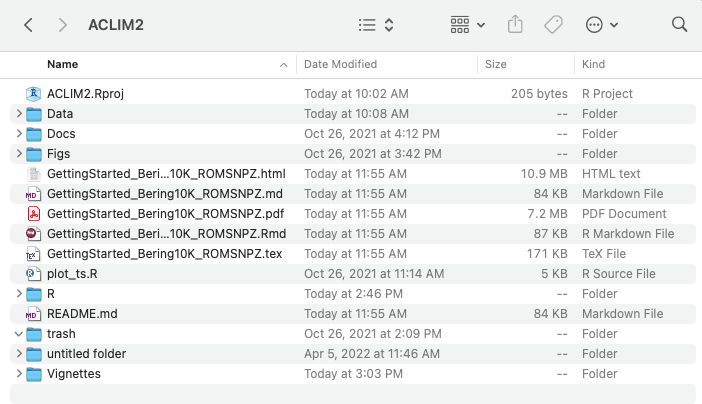
\includegraphics[width=1\textwidth,height=\textheight]{Figs/ACLIM_dir.png}

\hypertarget{option-3-use-git-commandline}{%
\subsubsection{Option 3: Use git
commandline}\label{option-3-use-git-commandline}}

If you have git installed and can work with it, this is the preferred
method as it preserves all directory structure and can aid in future
updating. Use this from a \textbf{terminal command line, not in R}, to
clone the full ACLIM2 directory and sub-directories:

\begin{Shaded}
\begin{Highlighting}[]
    \FunctionTok{git}\NormalTok{ clone https://github.com/kholsman/ACLIM2.git}
\end{Highlighting}
\end{Shaded}

\begin{center}\rule{0.5\linewidth}{0.5pt}\end{center}

\hypertarget{get-the-data}{%
\subsection{Get the data}\label{get-the-data}}

\textbf{Step 1){[} can skip if not using .nc files directly{]} } * Go to
the google drive and download the zipped file with the R data
\texttt{2022\_03\_07\_Rdata.zip}:

\begin{itemize}
\item
  \href{https://drive.google.com/drive/folders/11BQEfNEl9vvrN-V0LgS67XS4aLE9pNzz}{00\_ACLIM\_shared
  \textgreater{} 02\_Data \textgreater{} Newest\_Data(use this)
  \textgreater{} unzip\_and\_putin\_Data\_in\_folder.zip}
\item
  Unzip the folder and move the contents of the zipped folder to your
  local folder \texttt{ACLIM2/Data/in}.
\end{itemize}

\textbf{Step 2)} * Go to the google drive and download the zipped file
with the R ACLIM2 indices \texttt{ACLIM2\_indices.zip}:

\begin{itemize}
\item
  \href{https://drive.google.com/drive/folders/11BQEfNEl9vvrN-V0LgS67XS4aLE9pNzz}{00\_ACLIM\_shared
  \textgreater{} 02\_Data \textgreater{} Newest\_Data(use this)
  \textgreater{} unzip\_and\_putin\_Data\_out\_folder.zip}
\item
  Unzip the folder and move the contents of the zipped folder to your
  local folder \texttt{ACLIM2/Data/out}.
\end{itemize}

\hypertarget{set-up-the-workspace}{%
\subsection{Set up the Workspace}\label{set-up-the-workspace}}

Open R() and used `setwd()' to navigate to the root ACLIM2 folder (.e.g,
\textasciitilde/mydocuments/ACLIM2)

\begin{Shaded}
\begin{Highlighting}[]
    \CommentTok{\# set the workspace to your local ACLIM2 folder}
    \CommentTok{\# e.g., "/Users/kholsman/Documents/GitHub/ACLIM2"}
    \CommentTok{\# setwd( path.expand("\textasciitilde{}/Documents/GitHub/ACLIM2") )}
   
    \CommentTok{\# {-}{-}{-}{-}{-}{-}{-}{-}{-}{-}{-}{-}{-}{-}{-}{-}{-}{-}{-}{-}{-}{-}{-}{-}{-}{-}{-}{-}{-}{-}{-}{-}{-}{-}{-}{-}{-}{-}}
    \CommentTok{\# SETUP WORKSPACE}
\NormalTok{    tmstp  }\OtherTok{\textless{}{-}} \FunctionTok{format}\NormalTok{(}\FunctionTok{Sys.time}\NormalTok{(), }\StringTok{"\%Y\_\%m\_\%d"}\NormalTok{)}
\NormalTok{    main   }\OtherTok{\textless{}{-}} \FunctionTok{getwd}\NormalTok{()  }\CommentTok{\#"\textasciitilde{}/GitHub\_new/ACLIM2"}
    
    \CommentTok{\# loads packages, data, setup, etc.}
    \FunctionTok{suppressWarnings}\NormalTok{(}\FunctionTok{source}\NormalTok{(}\StringTok{"R/make.R"}\NormalTok{))}
\end{Highlighting}
\end{Shaded}

\begin{verbatim}
## ------------------------------
## ALIM2/R/setup.R settings 
## ------------------------------
## data_path            : D:/romsnpz/roms_for_public 
## Rdata_path           : D:/romsnpz/2022_10_17_Rdata/roms_for_public 
## redownload_level3_mox: FALSE 
## update.figs          : FALSE 
## load_gis             : FALSE 
## update.outputs       : TRUE 
## update.figs          : FALSE 
## dpiIN                : 150 
## update.figs          : FALSE 
## ------------------------------
## ------------------------------
## 
## The following datasets are public, please cite as Hermann et al. 2019 (v.H16) and Kearney et al. 2020 (v.K20) :
## B10K-H16_CMIP5_CESM_BIO_rcp85 
## B10K-H16_CMIP5_CESM_rcp45 
## B10K-H16_CMIP5_CESM_rcp85 
## B10K-H16_CMIP5_GFDL_BIO_rcp85 
## B10K-H16_CMIP5_GFDL_rcp45 
## B10K-H16_CMIP5_GFDL_rcp85 
## B10K-H16_CMIP5_MIROC_rcp45 
## B10K-H16_CMIP5_MIROC_rcp85 
## B10K-H16_CORECFS 
## B10K-K20_CORECFS 
## 
## The following datasets are still under embargo, please do not share outside of ACLIM:
## B10K-K20P19_CMIP6_cesm_historical 
## B10K-K20P19_CMIP6_cesm_ssp126 
## B10K-K20P19_CMIP6_cesm_ssp585 
## B10K-K20P19_CMIP6_gfdl_historical 
## B10K-K20P19_CMIP6_gfdl_ssp126 
## B10K-K20P19_CMIP6_gfdl_ssp585 
## B10K-K20P19_CMIP6_miroc_historical 
## B10K-K20P19_CMIP6_miroc_ssp126 
## B10K-K20P19_CMIP6_miroc_ssp585
\end{verbatim}

\begin{center}\rule{0.5\linewidth}{0.5pt}\end{center}

\hypertarget{read-this-before-you-start}{%
\section{Read this before you start}\label{read-this-before-you-start}}

\hypertarget{overview}{%
\subsection{Overview}\label{overview}}

The \href{https://github.com/kholsman/ACLIM2}{\textbf{ACLIM2 github
repository}} contains R code and Rdata files for working with
netcdf-format data generated from the
\href{https://beringnpz.github.io/roms-bering-sea}{\textbf{downscaled
ROMSNPZ modeling}} of the ROMSNPZ Bering Sea Ocean Modeling team; Drs.
Hermann, Cheng, Kearney, Pilcher,Ortiz, and Aydin. The code and R
resources described in this tutorial are maintained by
\href{mailto:kirstin.holsman@noaa.gov}{Kirstin Holsman} as part of
NOAA's
\href{https://www.fisheries.noaa.gov/alaska/ecosystems/alaska-climate-integrated-modeling-project}{\textbf{ACLIM
project}} for the Bering Sea. \emph{See
\href{https://www.frontiersin.org/articles/10.3389/fmars.2019.00775/full}{Hollowed
et al.~2020} for more information about the ACLIM project.}

\begin{center}\rule{0.5\linewidth}{0.5pt}\end{center}

This document provides an overview of accessing, plotting, and creating
bias corrected indices for ACLIM2 based on CMIP6 (embargoed for ACLIM2
users until 2023) and CMIP5 (publicly available) simulations. This guide
assumes analyses will take place in R() and that users have access to
the data folder within the ACLIM2 shared drive. For more information
also see the full tutorial (``GettingStarted\_Bering10K\_ROMSNPZ''
available at the bottom of
\href{https://github.com/kholsman/ACLIM2}{\textbf{this repo page}}.

\textbf{Important!} A few key things to know before getting started are
detailed below. Please review this information before getting started.

\hypertarget{romsnpz-versions}{%
\subsection{ROMSNPZ versions}\label{romsnpz-versions}}

\textbf{Important!} ACLIM1 CMIP5 and ACLIM2 CMIP5 and CMIP6 datasets use
different base models.

There are two versions of the ROMSNPZ model:

\begin{enumerate}
\def\labelenumi{\arabic{enumi}.}
\tightlist
\item
  ACLIM1 an older 10-depth layer model used for CMIP5 (``H-16'')
\item
  ACLIM2 a new 30-depth layer model used for CMIP6 (``K20'' or
  ``K20P19'')
\end{enumerate}

The models are not directly comparable, therefore the projections should
be bias corrected and recentered to baselines of hindcasts of each model
(forced by ``observed'' climate conditions). i.e.~CMIP5 and CMIP6 have
corresponding hindcasts:

\begin{enumerate}
\def\labelenumi{\arabic{enumi}.}
\tightlist
\item
  Hindcast for CMIP5 ``H19'' --\textgreater{} H16\_CORECFS
\item
  Hindcast for CMIP5 ``K20P19'' --\textgreater{} H16\_CORECFS
\item
  Hindcast for CMIP6 ``K20P19'' --\textgreater{} K20\_CORECFS
\end{enumerate}

In addition for CMIP6 ``historical'' runs are available for bias
correcting. We will use those below.

For a list of the available simulations for ACLIM enter the following in
R():

\begin{Shaded}
\begin{Highlighting}[]
    \CommentTok{\# list of the climate scenarios}
    \FunctionTok{data.frame}\NormalTok{(sim\_list)}
\end{Highlighting}
\end{Shaded}

\begin{verbatim}
##                              sim_list
## 1                    B10K-K20_CORECFS
## 2       B10K-H16_CMIP5_CESM_BIO_rcp85
## 3           B10K-H16_CMIP5_CESM_rcp45
## 4           B10K-H16_CMIP5_CESM_rcp85
## 5       B10K-H16_CMIP5_GFDL_BIO_rcp85
## 6           B10K-H16_CMIP5_GFDL_rcp45
## 7           B10K-H16_CMIP5_GFDL_rcp85
## 8          B10K-H16_CMIP5_MIROC_rcp45
## 9          B10K-H16_CMIP5_MIROC_rcp85
## 10                   B10K-H16_CORECFS
## 11       B10K-K20P19_CMIP5_CESM_rcp45
## 12       B10K-K20P19_CMIP5_CESM_rcp85
## 13       B10K-K20P19_CMIP5_GFDL_rcp45
## 14       B10K-K20P19_CMIP5_GFDL_rcp85
## 15      B10K-K20P19_CMIP5_MIROC_rcp45
## 16      B10K-K20P19_CMIP5_MIROC_rcp85
## 17  B10K-K20P19_CMIP6_cesm_historical
## 18      B10K-K20P19_CMIP6_cesm_ssp126
## 19      B10K-K20P19_CMIP6_cesm_ssp585
## 20  B10K-K20P19_CMIP6_gfdl_historical
## 21      B10K-K20P19_CMIP6_gfdl_ssp126
## 22      B10K-K20P19_CMIP6_gfdl_ssp585
## 23 B10K-K20P19_CMIP6_miroc_historical
## 24     B10K-K20P19_CMIP6_miroc_ssp126
## 25     B10K-K20P19_CMIP6_miroc_ssp585
\end{verbatim}

\hypertarget{romsnpz-variables}{%
\subsection{ROMSNPZ variables}\label{romsnpz-variables}}

For a list of the available variables from the ROMSNPZ:

\begin{Shaded}
\begin{Highlighting}[]
    \CommentTok{\# Metadata for variables}
\NormalTok{    (srvy\_var\_def[}\SpecialCharTok{{-}}\NormalTok{(}\DecValTok{1}\SpecialCharTok{:}\DecValTok{5}\NormalTok{),])}
\end{Highlighting}
\end{Shaded}

\begin{verbatim}
##                    name                            units
## 6                   Ben                        mg C m^-2
## 7                DetBen                        mg C m^-2
## 8                  Hsbl                            meter
## 9                IceNH4                      mmol N m^-3
## 10               IceNO3                      mmol N m^-3
## 11               IcePhL                        mg C m^-3
## 12                 aice                                 
## 13                 hice                            meter
## 14               shflux                     watt meter-2
## 15               ssflux                   meter second-1
## 16       Cop_integrated                    (mg C m^-3)*m
## 17        Cop_surface5m                        mg C m^-3
## 18      EupO_integrated                    (mg C m^-3)*m
## 19       EupO_surface5m                        mg C m^-3
## 20      EupS_integrated                    (mg C m^-3)*m
## 21       EupS_surface5m                        mg C m^-3
## 22        Iron_bottom5m                  micromol Fe m-3
## 23      Iron_integrated              (micromol Fe m-3)*m
## 24       Iron_surface5m                  micromol Fe m-3
## 25       Jel_integrated                    (mg C m^-3)*m
## 26        Jel_surface5m                        mg C m^-3
## 27       MZL_integrated                    (mg C m^-3)*m
## 28        MZL_surface5m                        mg C m^-3
## 29      NCaO_integrated                    (mg C m^-3)*m
## 30       NCaO_surface5m                        mg C m^-3
## 31      NCaS_integrated                    (mg C m^-3)*m
## 32       NCaS_surface5m                        mg C m^-3
## 33         NH4_bottom5m                      mmol N m^-3
## 34       NH4_integrated                  (mmol N m^-3)*m
## 35        NH4_surface5m                      mmol N m^-3
## 36         NO3_bottom5m                      mmol N m^-3
## 37       NO3_integrated                  (mmol N m^-3)*m
## 38        NO3_surface5m                      mmol N m^-3
## 39       PhL_integrated                    (mg C m^-3)*m
## 40        PhL_surface5m                        mg C m^-3
## 41       PhS_integrated                    (mg C m^-3)*m
## 42        PhS_surface5m                        mg C m^-3
## 43  prod_Cop_integrated                   mg C m^-2 d^-1
## 44 prod_EupO_integrated                   mg C m^-2 d^-1
## 45 prod_EupS_integrated                   mg C m^-2 d^-1
## 46  prod_Eup_integrated (milligram carbon meter-3 d-1)*m
## 47  prod_Jel_integrated                   mg C m^-2 d^-1
## 48  prod_MZL_integrated                   mg C m^-2 d^-1
## 49 prod_NCaO_integrated                   mg C m^-2 d^-1
## 50 prod_NCaS_integrated                   mg C m^-2 d^-1
## 51  prod_NCa_integrated (milligram carbon meter-3 d-1)*m
## 52  prod_PhL_integrated                   mg C m^-2 d^-1
## 53  prod_PhS_integrated                   mg C m^-2 d^-1
## 54       salt_surface5m                                 
## 55        temp_bottom5m                          Celsius
## 56      temp_integrated                      (Celsius)*m
## 57       temp_surface5m                          Celsius
## 58       uEast_bottom5m                   meter second-1
## 59      uEast_surface5m                   meter second-1
## 60      vNorth_bottom5m                   meter second-1
## 61     vNorth_surface5m                   meter second-1
##                                                       longname
## 6                                Benthic infauna concentration
## 7                               Benthic detritus concentration
## 8                      depth of oceanic surface boundary layer
## 9                                   Ice ammonium concentration
## 10                                   Ice nitrate concentration
## 11                                     Ice algae concentration
## 12                             fraction of cell covered by ice
## 13                               average ice thickness in cell
## 14                                       surface net heat flux
## 15                           surface net salt flux, (E-P)*SALT
## 16          Small copepod concentration, integrated over depth
## 17                Small copepod concentration, surface 5m mean
## 18    Offshore euphausiid concentration, integrated over depth
## 19          Offshore euphausiid concentration, surface 5m mean
## 20    On-shelf euphausiid concentration, integrated over depth
## 21          On-shelf euphausiid concentration, surface 5m mean
## 22                          iron concentration, bottom 5m mean
## 23                   iron concentration, integrated over depth
## 24                         iron concentration, surface 5m mean
## 25              Jellyfish concentration, integrated over depth
## 26                    Jellyfish concentration, surface 5m mean
## 27       Microzooplankton concentration, integrated over depth
## 28             Microzooplankton concentration, surface 5m mean
## 29 Offshore large copepod concentration, integrated over depth
## 30       Offshore large copepod concentration, surface 5m mean
## 31 On-shelf large copepod concentration, integrated over depth
## 32       On-shelf large copepod concentration, surface 5m mean
## 33                      Ammonium concentration, bottom 5m mean
## 34               Ammonium concentration, integrated over depth
## 35                     Ammonium concentration, surface 5m mean
## 36                       Nitrate concentration, bottom 5m mean
## 37                Nitrate concentration, integrated over depth
## 38                      Nitrate concentration, surface 5m mean
## 39    Large phytoplankton concentration, integrated over depth
## 40          Large phytoplankton concentration, surface 5m mean
## 41    Small phytoplankton concentration, integrated over depth
## 42          Small phytoplankton concentration, surface 5m mean
## 43                  Cop net production rate, summed over depth
## 44                 EupO net production rate, summed over depth
## 45                 EupS net production rate, summed over depth
## 46     secondary production Euphausiids, integrated over depth
## 47                  Jel net production rate, summed over depth
## 48                  MZL net production rate, summed over depth
## 49                 NCaO net production rate, summed over depth
## 50                 NCaS net production rate, summed over depth
## 51      secondary production Neocalanus, integrated over depth
## 52                  PhL net production rate, summed over depth
## 53                  PhS net production rate, summed over depth
## 54                                   salinity, surface 5m mean
## 55                       potential temperature, bottom 5m mean
## 56                potential temperature, integrated over depth
## 57                      potential temperature, surface 5m mean
## 58           u-momentum component, geo-rotated, bottom 5m mean
## 59          u-momentum component, geo-rotated, surface 5m mean
## 60           v-momentum component, geo-rotated, bottom 5m mean
## 61          v-momentum component, geo-rotated, surface 5m mean
\end{verbatim}

\hypertarget{data-outputs}{%
\subsection{Data outputs}\label{data-outputs}}

\textbf{Important!} There are 2 types of post-processed data available
for use in ACLIM.

The ROMSNPZ team has developed a process to provide standardized
post-processed outputs from the large (and non-intuitive) ROMSNPZ grid.
These have been characterized as:

\begin{enumerate}
\def\labelenumi{\arabic{enumi}.}
\tightlist
\item
  Level 1 (original ROMSNPZ U,V, grid, not rotated or corrected)\\
\item
  Level 2 (lat long bi-weekly high res versions, shouldn't be needed and
  are difficult to work with)\\
\item
  \textbf{Level 3 indices (depth corrected and area weighted means for
  each model variable; i.e., what we will mostly use) }

  \begin{enumerate}
  \def\labelenumii{\alph{enumii}.}
  \tightlist
  \item
    ``ACLIMsurveyrep\_'': groundifsh survey replicated (replicated in
    space and time)
  \item
    ``ACLIMregion\_'': weekly strata based averages
  \end{enumerate}
\end{enumerate}

To get more information about each of these level 3 datasets enter this
in R:

\begin{Shaded}
\begin{Highlighting}[]
    \CommentTok{\# Metadata for Weekly ("ACLIMregion\_...") indices}
    \FunctionTok{head}\NormalTok{(all\_info1)}
\end{Highlighting}
\end{Shaded}

\begin{verbatim}
##                            name                    Type B10KVersion  CMIP  GCM
## 1 B10K-H16_CMIP5_CESM_BIO_rcp85 Weekly regional indices         H16 CMIP5 CESM
## 2     B10K-H16_CMIP5_CESM_rcp45 Weekly regional indices         H16 CMIP5 CESM
## 3     B10K-H16_CMIP5_CESM_rcp85 Weekly regional indices         H16 CMIP5 CESM
## 4 B10K-H16_CMIP5_GFDL_BIO_rcp85 Weekly regional indices         H16 CMIP5 GFDL
## 5     B10K-H16_CMIP5_GFDL_rcp45 Weekly regional indices         H16 CMIP5 GFDL
## 6     B10K-H16_CMIP5_GFDL_rcp85 Weekly regional indices         H16 CMIP5 GFDL
##     BIO Carbon_scenario               Start                 End nvars
## 1  TRUE           rcp85 2006-01-22 12:00:00 2099-12-27 12:00:00    59
## 2 FALSE           rcp45 2006-01-22 12:00:00 2081-02-16 12:00:00    59
## 3 FALSE           rcp85 2006-01-22 12:00:00 2099-12-27 12:00:00    59
## 4  TRUE           rcp85 2006-01-22 12:00:00 2099-12-27 12:00:00    59
## 5 FALSE           rcp45 2006-01-22 12:00:00 2099-12-27 12:00:00    59
## 6 FALSE           rcp85 2006-01-22 12:00:00 2099-12-27 12:00:00    59
\end{verbatim}

\begin{Shaded}
\begin{Highlighting}[]
    \CommentTok{\# Metadata for Weekly ("ACLIMsurveyrep\_...") indices}
    \FunctionTok{head}\NormalTok{(all\_info2)}
\end{Highlighting}
\end{Shaded}

\begin{verbatim}
##                            name              Type B10KVersion  CMIP  GCM   BIO
## 1 B10K-H16_CMIP5_CESM_BIO_rcp85 Survey replicated         H16 CMIP5 CESM  TRUE
## 2     B10K-H16_CMIP5_CESM_rcp45 Survey replicated         H16 CMIP5 CESM FALSE
## 3     B10K-H16_CMIP5_CESM_rcp85 Survey replicated         H16 CMIP5 CESM FALSE
## 4 B10K-H16_CMIP5_GFDL_BIO_rcp85 Survey replicated         H16 CMIP5 GFDL  TRUE
## 5     B10K-H16_CMIP5_GFDL_rcp45 Survey replicated         H16 CMIP5 GFDL FALSE
## 6     B10K-H16_CMIP5_GFDL_rcp85 Survey replicated         H16 CMIP5 GFDL FALSE
##   Carbon_scenario Start  End nvars
## 1           rcp85  1970 2100    60
## 2           rcp45  1970 2100    60
## 3           rcp85  1970 2100    60
## 4           rcp85  1970 2100    60
## 5           rcp45  1970 2100    60
## 6           rcp85  1970 2100    60
\end{verbatim}

\hypertarget{indices-bias-correction}{%
\section{Indices \& bias correction}\label{indices-bias-correction}}

\emph{ACLIM2 Indices}

The next step creates ACLIM2 indices (i.e., Level4) based on the Level3
output for each hindcast, historical run, and CMIP6 projection. The
script below then bias corrects each index using the historical run and
recenters the projection on the corresponding hindcast (such that
projections are \(\Delta\) from historical mean values for the reference
period \texttt{deltayrs\ \ \ \ \ \textless{}-\ 1970:2000} ).

\emph{NESB \& SEBS averaged indices} The average water column values for
each variable from the ROMSNPZ model strata x weekly Level2 outputs
(`ACLIMregion') was calculated and used to calculate the strata-area
weighted mean value for the NEBS and SEBS weekly, monthly, seasonally,
and annually. Similarly, for survey replicated (`ACLIMsurveyrep') Level2
outputs the average water column value for each variable at each station
was calculated used to calculate the strata-area weighted mean value for
the NEBS and SEBS annually. These indices were calculate for hindcast,
historical, and projection scenarios, and used to bias correct the
projections. More information on the methods for each can be found in
the tabs below and the code immediately following this section will
re-generate the bias corrected indices. All of the bias corrected
outputs can be found in the ``Data/out/CMIP6'' folder.

\begin{figure}
\centering
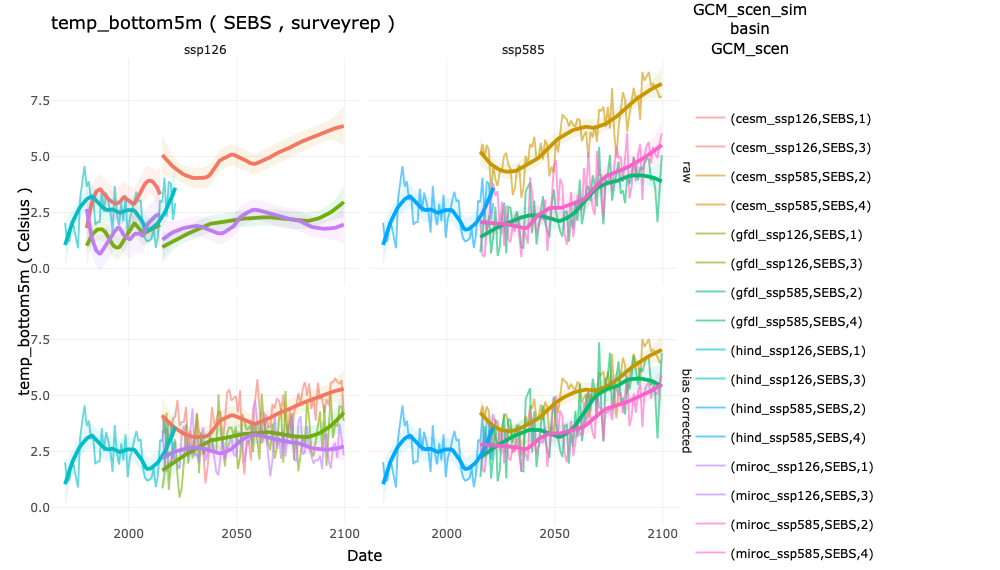
\includegraphics[width=0.75\textwidth,height=\textheight]{Figs/biascorrected_temp2.png}
\caption{\textbf{Raw (top row) and bias corrected (bottom row)bottom
temperature indices based on survey replicated Level3 outputs for the
SEBS}}
\end{figure}

\textbf{Important!} Note that for projections the `mn\_val' represents
raw mean values, while `val\_biascorrected' is the bias corrected
mn\_val (should be used instead of the raw values). In all cases, for
variables that are log-normally distributed (cannot be \textless{} 0),
the ln(mn\_val) were used to bias correct and were then back transformed
to non-log space after correction:

For normally distributed variables (\(Y\)):
\[{Y}^{fut'}_{t,k} =\bar{Y}^{hind}_{k,\bar{T}} +\left( \frac{\sigma^{hind}_{k,\bar{T}}}{\sigma^{hist}_{k,\bar{T}}}*({Y}^{fut}_{t,k}-\bar{Y}^{hist}_{k,\bar{T}})  \right )\]

where \(\bar{Y}^{fut'}_{y,k}\) is the bias corrected varable \(k\) value
for time-step \(t\) (e.g., year, month, or season),
\(\bar{Y}^{hind}_{k,\bar{T}}\) is the mean value of the variable \(k\)
during the reference period \(\bar{T}=[1980,2013]\) from the hindcast
model, \(\sigma^{hind}_{k,\bar{T}}\) is the standard deviation of the
hindcast during the reference period \(\bar{T}\),
\(\sigma^{hist}_{k,\bar{T}}\) is the standard deviation of the
historical run during tje reference period, \({Y}^{fut}_{t,k}\) is the
value of the variable from the projection at time-step \(t\) and
\(\bar{Y}^{hist}_{k,\bar{T}}\) is the average value from the historical
run during reference period \(\bar{T}\).

For log-normally distributed variables(\(Y\)):
\[{Y}^{fut'}_{y,k} =e^{\ln\bar{Y}^{hind}_{k,\bar{T}} +\left( \frac{\hat{\sigma}^{hind}_{k,\bar{T}}}{\hat{\sigma}^{hist}_{k,\bar{T}}}*(\ln{Y}^{fut}_{t,k}-\ln\bar{Y}^{hist}_{k,\bar{T}})  \right )}\],
where \(\hat\sigma^{hist}_{k,\bar{T}}\) and
\(\hat\sigma^{hind}_{k,\bar{T}}\) are the standard deviation of the
\(\ln\bar{Y}^{hist}_{k,t}\) and \(\ln\bar{Y}^{hind}_{k,t}\) during the
reference period \(\hat{T}\) (respectively).

\hypertarget{weekly-indices}{%
\subsection{Weekly indices}\label{weekly-indices}}

Uses the strata x weekly data (`ACLIMregion') to generate
strata-specific averages in order to generate the strata area-weighted
averages for each week \(w\) each year \(y\).

\[\bar{Y}_{w,y,k}= \frac{\sum^{n_s}_{l}(\frac{1}{n_i}\sum^{n_t}_{t}Y_{k,w,y,s,t})*A_s} {\sum^{n_s}_{s}{A_s}}\],
where \(Y_{k,w,y,s,t}\) is the value of the variable \(k\) in strata
\(s\) at time \(t\) in year \(y\), \(A_s\) is the area of strata \(s\),
\(n_i\) is the number of stations in strata \(s\), and \(n_s\) is the
number of strata \(s\) in each basin (NEBS or SEBS).

\(\bar{Y}_{w,y,k}\) was calculated for the hindcast, historical run, and
projection time-series. For projections \(\bar{Y}_{w,y,k}\) was bias
corrected using the corresponding historical and hindcast values such
that:

\[\bar{Y}^{fut'}_{w,y,k} =\bar{Y}^{hind}_{w,k} +\left( \frac{\sigma^{hind}_{w,k}}{\sigma^{hist}_{w,k}}*(\bar{Y}^{fut}_{w,y,k}-\bar{Y}^{hist}_{w,k})  \right )\],
where \(\bar{Y}^{hist}_{w,k}\) and \(\bar{Y}^{hind}_{w,k}\) are the
average historical weekly values across years in the period (1980 to
2012 ; adjustable in \texttt{R/setup.R}).

\hypertarget{monthly-indices}{%
\subsection{Monthly indices}\label{monthly-indices}}

Uses the strata x weekly data (`ACLIMregion') to generate
strata-specific averages in order to generate the strata area-weighted
averages for each month \(m\) each year \(y\).

\[\bar{Y}_{m,y,k}= \frac{1}{n_w}\sum^{n_w}_{w}\bar{Y}_{w,y,k}\], where
\(\bar{Y}_{w,y,k}\) are the weekly average indices for variable \(k\) in
year \(y\) from the previous step ,\(n_w\) is the number of weeks in
each month \(m\).

\(\bar{Y}_{m,y,k}\) was calculated for the hindcast, historical run, and
projection time-series. For projections \(\bar{Y}_{m,y,k}\) was bias
corrected using the corresponding historical and hindcast values such
that:

\[\bar{Y}^{fut'}_{m,y,k} =\bar{Y}^{hind}_{m,k} +\left( \frac{\sigma^{hind}_{m,k}}{\sigma^{hist}_{m,k}}*(\bar{Y}^{fut}_{m,y,k}-\bar{Y}^{hist}_{m,k})  \right )\],
where \(\bar{Y}^{hist}_{m,k}\) and \(\bar{Y}^{hind}_{m,k}\) are the
average historical monthly values across years in the period (1980 to
2012 ; adjustable in \texttt{R/setup.R}).

\hypertarget{seasonal-indices}{%
\subsection{Seasonal indices}\label{seasonal-indices}}

Uses the strata x weekly data (`ACLIMregion') to generate
strata-specific averages in order to generate the strata area-weighted
averages for each season \(l\) each year \(y\).

\[\bar{Y}_{l,y,k}= \frac{1}{n_w}\sum^{n_w}_{w}\bar{Y}_{w,y,k}\], where
\(\bar{Y}_{w,y,k}\) are the weekly average indices for variable \(k\) in
year \(y\) from the previous step ,\(n_w\) is the number of weeks in
each season \(l\).

\(\bar{Y}_{l,y,k}\) was calculated for the hindcast, historical run, and
projection time-series. For projections \(\bar{Y}_{l,y,k}\) was bias
corrected using the corresponding historical and hindcast values such
that:

\[\bar{Y}^{fut'}_{l,y,k} =\bar{Y}^{hind}_{l,k} +\left( \frac{\sigma^{hind}_{l,k}}{\sigma^{hist}_{l,k}}*(\bar{Y}^{fut}_{l,y,k}-\bar{Y}^{hist}_{l,k})  \right )\],
where \(\bar{Y}^{hist}_{l,k}\) and \(\bar{Y}^{hind}_{l,k}\) are the
average historical seasonal values across years in the reference period
(1980 to 2012 ; adjustable in \texttt{R/setup.R}).

\hypertarget{annual-indices}{%
\subsection{Annual indices}\label{annual-indices}}

Uses the strata x weekly data (`ACLIMregion') to generate
strata-specific averages in order to generate the strata area-weighted
averages for each season \(l\) each year \(y\).

\[\bar{Y}_{y,k}= \frac{1}{n_w}\sum^{n_w}_{w}\bar{Y}_{w,y,k}\], where
\(\bar{Y}_{w,y,k}\) are the weekly average indices for variable \(k\) in
year \(y\) from the previous step ,\(n_w\) is the number of weeks in
each year \(y\).

\(\bar{Y}_{y,k}\) was calculated for the hindcast, historical run, and
projection time-series. For projections \(\bar{Y}_{y,k}\) was bias
corrected using the corresponding historical and hindcast values such
that:

\[\bar{Y}^{fut'}_{y,k} =\bar{Y}^{hind}_{k} +\left( \frac{\sigma^{hind}_{k}}{\sigma^{hist}_{k}}*(\bar{Y}^{fut}_{y,k}-\bar{Y}^{hist}_{k})  \right )\],
where \(\bar{Y}^{hind}_{k}\) and \(\bar{Y}^{hist}_{k}\) are the average
historical values across years in the reference period (1980 to 2012 ;
adjustable in \texttt{R/setup.R}).

\hypertarget{annual-survey-rep.-indices}{%
\subsection{Annual survey rep.
indices}\label{annual-survey-rep.-indices}}

Uses the station specific survey replicated (in time and space) data
(`ACLIMsurveyrep') to generate strata-specific averages in order to
generate the strata area-weighted averages for each year \(y\).

\[\bar{Y}_{y,k}= \frac{\sum^{n_s}_{l}(\frac{1}{n_i}\sum^{n_i}_{i}Y_{k,y,s,i})*A_s} {\sum^{n_s}_{s}{A_s}}\],
where \(Y_{k,y,s,i}\) is the value of the variable \(k\) at station
\(i\) in strata \(s\) in year \(y\), \(A_s\) is the area of strata
\(s\), \(n_i\) is the number of stations in strata \(s\), and \(n_s\) is
the number of strata \(s\) in each basin (NEBS or SEBS).

\(\bar{Y}_{y,k}\) was calculated for the hindcast, historical run, and
projection time-series. For projections \(\bar{Y}_{y,k}\) was bias
corrected using the corresponding historical and hindcast values such
that:

\[\bar{Y}^{fut'}_{y,k} =\bar{Y}^{hind}_{k} +\left( \frac{\sigma^{hind}_{k}}{\sigma^{hist}_{k}}*(\bar{Y}^{fut}_{y,k}-\bar{Y}^{hist}_{k})  \right )\],
where \(\bar{Y}^{hind}_{k}\) and \(\bar{Y}^{hist}_{k}\) are the average
historical values across years in the reference period (1980 to 2012 ;
adjustable in \texttt{R/setup.R}).

Appendix A includes the code used to generate the ACLIM2 indices and
bias correct them. That code can be run to re-make the indices if you
like but takes approx 30 mins a CMIP to run.

\hypertarget{plot-concat-indices}{%
\section{Plot \& concat Indices}\label{plot-concat-indices}}

The following code will open an interactive shiny() app for exploring
the indices. You can also view this online at
(kkh2022.shinyapps.io/ACLIM2\_indices){[}\url{https://kkh2022.shinyapps.io/ACLIM2_indices/}{]}.

\begin{Shaded}
\begin{Highlighting}[]
\NormalTok{  tmpwd}\OtherTok{\textless{}{-}}\FunctionTok{getwd}\NormalTok{()}
  \FunctionTok{setwd}\NormalTok{(}\StringTok{"R/shiny\_aclim/ACLIM2\_indices"}\NormalTok{)  }
\NormalTok{  shiny}\SpecialCharTok{::}\FunctionTok{runApp}\NormalTok{(}\StringTok{"app.R"}\NormalTok{)}
  \FunctionTok{setwd}\NormalTok{(tmpwd)}
  \CommentTok{\# alternatively you can extract the data you want using the get\_var()function}
  
\NormalTok{  df }\OtherTok{\textless{}{-}} \FunctionTok{get\_var}\NormalTok{(}\AttributeTok{typeIN =} \StringTok{"annual"}\NormalTok{,}\AttributeTok{plotvar =} \StringTok{"temp\_bottom5m"}\NormalTok{,}\AttributeTok{plothist =}\NormalTok{ F)}
  
\NormalTok{  df}\SpecialCharTok{$}\NormalTok{plot}
  \FunctionTok{head}\NormalTok{(df}\SpecialCharTok{$}\NormalTok{dat)}
\end{Highlighting}
\end{Shaded}

\begin{figure}
\centering
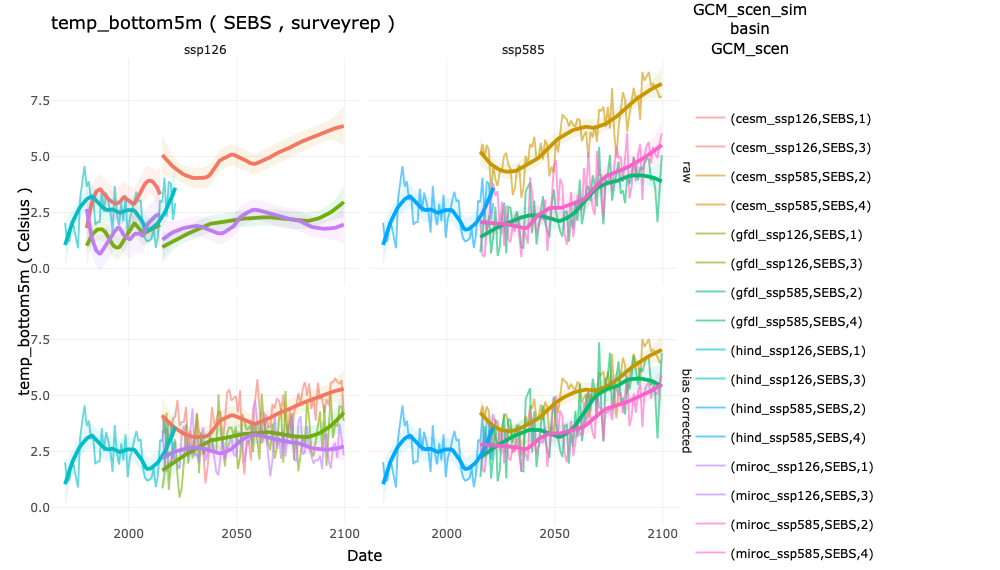
\includegraphics[width=1\textwidth,height=\textheight]{Figs/biascorrected_temp2.png}
\caption{``Raw (top row) and bias corrected (bottom row)bottom
temperature indices based on survey replicated Level3 outputs for the
SEBS''}
\end{figure}

\hypertarget{nrs-indices-andruxe9}{%
\subsection{NRS indices (André)}\label{nrs-indices-andruxe9}}

\begin{Shaded}
\begin{Highlighting}[]
    \FunctionTok{suppressMessages}\NormalTok{(}\FunctionTok{source}\NormalTok{(}\StringTok{"R/make.R"}\NormalTok{))}
    \CommentTok{\# preview possible variables}
    
    \CommentTok{\#load(file = "Data/out/weekly\_vars\_C.Rdata")}
    \FunctionTok{load}\NormalTok{(}\AttributeTok{file =} \StringTok{"Data/out/weekly\_vars.Rdata"}\NormalTok{)}
    \CommentTok{\#load(file = "Data/out/srvy\_vars\_C.Rdata")}
    \FunctionTok{load}\NormalTok{(}\AttributeTok{file =} \StringTok{"Data/out/srvy\_vars.Rdata"}\NormalTok{)}
    
    \FunctionTok{load}\NormalTok{(}\FunctionTok{paste0}\NormalTok{(}\StringTok{"Data/out/K20P19\_CMIP6/allEBS\_means/ACLIM\_annual\_hind\_mn.Rdata"}\NormalTok{))}
\NormalTok{    varall  }\OtherTok{\textless{}{-}} \FunctionTok{unique}\NormalTok{(ACLIM\_annual\_hind}\SpecialCharTok{$}\NormalTok{var)}
\NormalTok{    varall}
    
\NormalTok{    scens   }\OtherTok{\textless{}{-}} \FunctionTok{c}\NormalTok{(}\StringTok{"ssp126"}\NormalTok{, }\StringTok{"ssp585"}\NormalTok{)}
\NormalTok{    GCMs    }\OtherTok{\textless{}{-}} \FunctionTok{c}\NormalTok{(}\StringTok{"miroc"}\NormalTok{, }\StringTok{"gfdl"}\NormalTok{, }\StringTok{"cesm"}\NormalTok{ )}
\NormalTok{    varlist }\OtherTok{\textless{}{-}} \FunctionTok{c}\NormalTok{(}\StringTok{"temp\_bottom5m"}\NormalTok{, }\StringTok{"fracbelow2"}\NormalTok{, }\StringTok{"uEast\_surface5m"}\NormalTok{, }\StringTok{"vNorth\_surface5m"}\NormalTok{)}

    \CommentTok{\# get the variable you want:}
\NormalTok{    df }\OtherTok{\textless{}{-}} \FunctionTok{get\_var}\NormalTok{( }\AttributeTok{typeIN    =} \StringTok{"annual"}\NormalTok{, }
                   \AttributeTok{plotvar   =}\NormalTok{ varlist[}\DecValTok{3}\NormalTok{],}
                   \AttributeTok{bcIN      =} \StringTok{"raw"}\NormalTok{,}
                   \AttributeTok{CMIPIN    =} \StringTok{"K20P19\_CMIP6"}\NormalTok{, }
                   \AttributeTok{plothist  =}\NormalTok{ T,  }\CommentTok{\# ignore the hist runs}
                   \AttributeTok{removeyr1 =}\NormalTok{ T)  }\CommentTok{\# "Remove first year of projection ( burn in)")}
    
\NormalTok{    df}\SpecialCharTok{$}\NormalTok{plot}\SpecialCharTok{+}\FunctionTok{coord\_cartesian}\NormalTok{(}\AttributeTok{ylim =} \FunctionTok{c}\NormalTok{(}\DecValTok{0}\NormalTok{, }\DecValTok{7}\NormalTok{)) }
\end{Highlighting}
\end{Shaded}

\begin{center}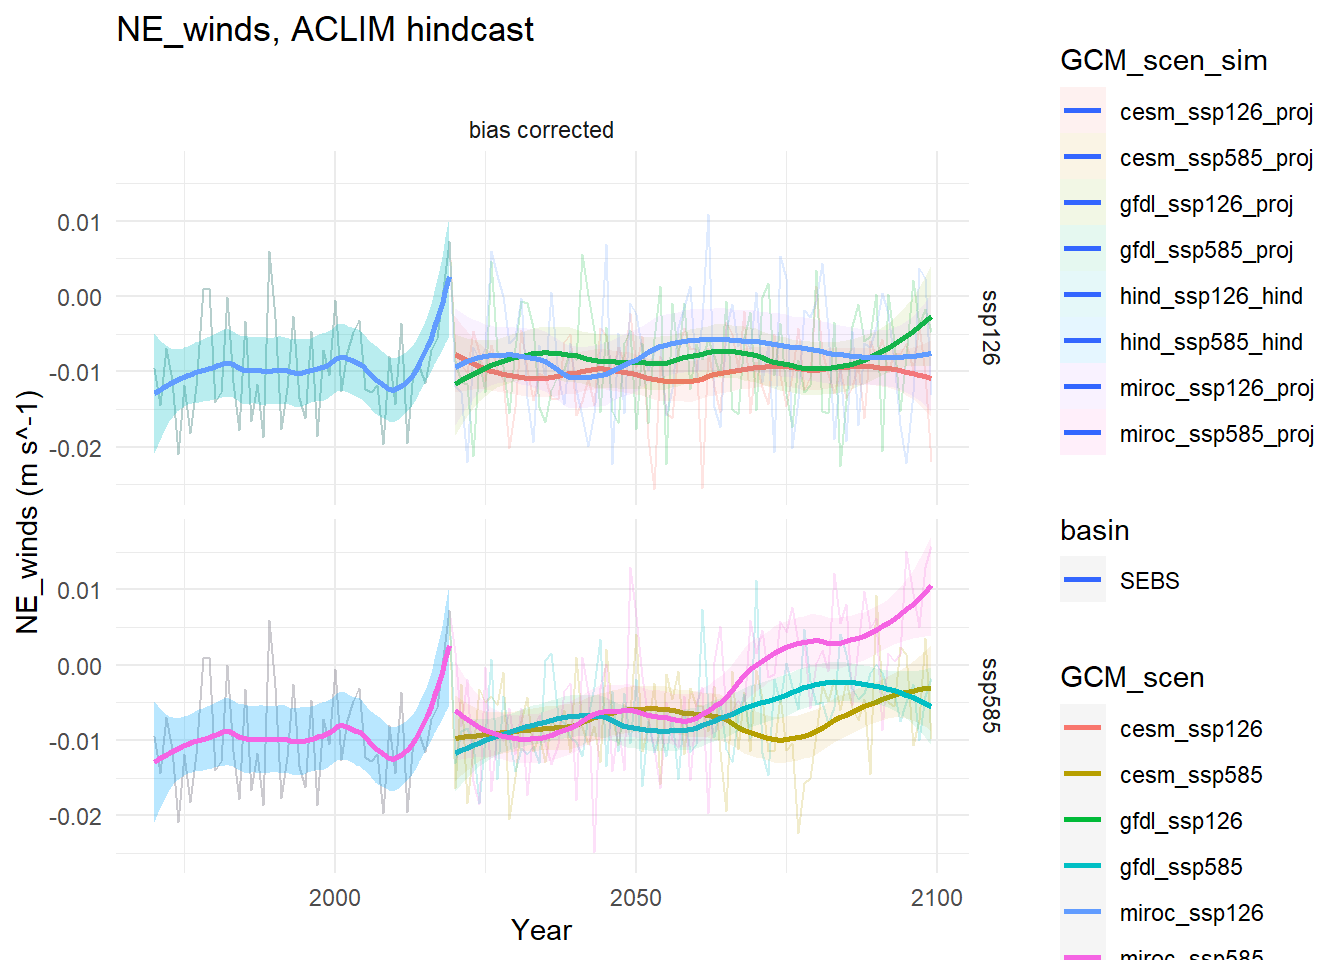
\includegraphics{ACLIM2_quickStart_files/figure-latex/nrs-1} \end{center}

\begin{Shaded}
\begin{Highlighting}[]
    \FunctionTok{head}\NormalTok{(df}\SpecialCharTok{$}\NormalTok{dat)}
\end{Highlighting}
\end{Shaded}

\hypertarget{continuous-timeseries-of-hind-fut}{%
\subsection{Continuous timeseries of hind +
fut}\label{continuous-timeseries-of-hind-fut}}

\begin{Shaded}
\begin{Highlighting}[]
    \CommentTok{\# get the variable you want:}
\NormalTok{    df }\OtherTok{\textless{}{-}} \FunctionTok{get\_var}\NormalTok{( }\AttributeTok{typeIN    =} \StringTok{"annual"}\NormalTok{, }
                   \AttributeTok{plotvar   =} \StringTok{"pH\_depthavg"}\NormalTok{,}
                   \AttributeTok{bcIN      =} \StringTok{"bias corrected"}\NormalTok{,}
                   \AttributeTok{CMIPIN    =} \StringTok{"K20P19\_CMIP6"}\NormalTok{, }
                   \AttributeTok{plothist  =}\NormalTok{ F,  }\CommentTok{\# ignore the hist runs}
                   \AttributeTok{removeyr1 =}\NormalTok{ T)  }\CommentTok{\# "Remove first year of projection ( burn in)")}
    
\NormalTok{    df}\SpecialCharTok{$}\NormalTok{plot}
\end{Highlighting}
\end{Shaded}

\begin{center}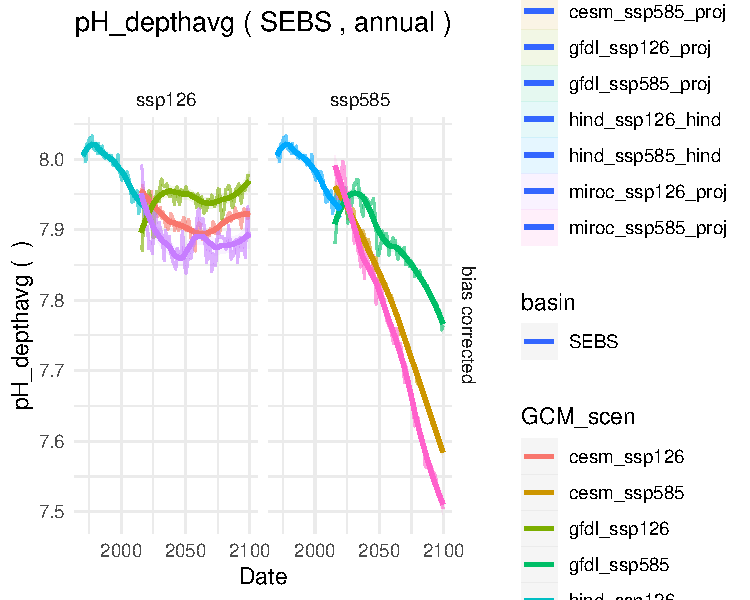
\includegraphics{ACLIM2_quickStart_files/figure-latex/ts-1} \end{center}

\begin{Shaded}
\begin{Highlighting}[]
    \FunctionTok{head}\NormalTok{(df}\SpecialCharTok{$}\NormalTok{dat)}
    
\CommentTok{\# concat the hind and fut runs by removing years from projection}
\NormalTok{maxDin }\OtherTok{\textless{}{-}} \FunctionTok{max}\NormalTok{(}\FunctionTok{as.vector}\NormalTok{(df}\SpecialCharTok{$}\NormalTok{dat}\SpecialCharTok{\%\textgreater{}\%}
\NormalTok{                          dplyr}\SpecialCharTok{::}\FunctionTok{filter}\NormalTok{(sim\_type}\SpecialCharTok{==}\StringTok{"hind"}\NormalTok{)}\SpecialCharTok{\%\textgreater{}\%}\FunctionTok{ungroup}\NormalTok{()}\SpecialCharTok{\%\textgreater{}\%}
\NormalTok{                          dplyr}\SpecialCharTok{::}\FunctionTok{select}\NormalTok{(mnDate))[[}\DecValTok{1}\NormalTok{]])}

\NormalTok{newdat }\OtherTok{\textless{}{-}} \FunctionTok{stitchTS}\NormalTok{(}\AttributeTok{dat =}\NormalTok{ df}\SpecialCharTok{$}\NormalTok{dat,}
                 \AttributeTok{maxD  =}\NormalTok{ maxDin)}

\CommentTok{\# newdat has the full set of data}
\CommentTok{\# select miroc\_ssp126}
\FunctionTok{head}\NormalTok{(newdat}\SpecialCharTok{\%\textgreater{}\%}\NormalTok{dplyr}\SpecialCharTok{::}\FunctionTok{filter}\NormalTok{(GCM\_scen}\SpecialCharTok{==}\FunctionTok{paste0}\NormalTok{(GCMs[}\DecValTok{1}\NormalTok{],}\StringTok{"\_"}\NormalTok{,scens[}\DecValTok{1}\NormalTok{])))}
\FunctionTok{tail}\NormalTok{(newdat}\SpecialCharTok{\%\textgreater{}\%}\NormalTok{dplyr}\SpecialCharTok{::}\FunctionTok{filter}\NormalTok{(GCM\_scen}\SpecialCharTok{==}\FunctionTok{paste0}\NormalTok{(GCMs[}\DecValTok{1}\NormalTok{],}\StringTok{"\_"}\NormalTok{,scens[}\DecValTok{1}\NormalTok{])))}

\NormalTok{pp  }\OtherTok{\textless{}{-}}  \FunctionTok{ggplot}\NormalTok{(newdat) }\SpecialCharTok{+}
        \FunctionTok{geom\_line}\NormalTok{(}\FunctionTok{aes}\NormalTok{(}\AttributeTok{x=}\NormalTok{mnDate,}\AttributeTok{y=}\NormalTok{mn\_val,}\AttributeTok{color=}\NormalTok{ GCM\_scen, }\AttributeTok{linetype =}\NormalTok{ basin),}
                    \AttributeTok{alpha =} \FloatTok{0.6}\NormalTok{,}\AttributeTok{show.legend =} \ConstantTok{FALSE}\NormalTok{) }\SpecialCharTok{+}
        \FunctionTok{geom\_smooth}\NormalTok{(}\FunctionTok{aes}\NormalTok{(}\AttributeTok{x =}\NormalTok{ mnDate, }
                        \AttributeTok{y =}\NormalTok{ mn\_val,}
                        \AttributeTok{color    =}\NormalTok{ GCM\_scen,}
                        \AttributeTok{fill     =}\NormalTok{ GCM\_scen,}
                        \AttributeTok{linetype =}\NormalTok{ basin),}
                    \AttributeTok{alpha       =} \FloatTok{0.1}\NormalTok{,}
                    \AttributeTok{method      =} \StringTok{"loess"}\NormalTok{,}
                    \AttributeTok{formula     =} \StringTok{\textquotesingle{}y \textasciitilde{} x\textquotesingle{}}\NormalTok{,}
                    \AttributeTok{span        =}\NormalTok{ .}\DecValTok{5}\NormalTok{,}
                    \AttributeTok{show.legend =}\NormalTok{ T) }\SpecialCharTok{+}
          \FunctionTok{theme\_minimal}\NormalTok{() }\SpecialCharTok{+} 
          \FunctionTok{labs}\NormalTok{(}\AttributeTok{x =} \StringTok{"Date"}\NormalTok{,}
               \AttributeTok{y =} \FunctionTok{paste}\NormalTok{(newdat}\SpecialCharTok{$}\NormalTok{var[}\DecValTok{1}\NormalTok{],}\StringTok{"("}\NormalTok{,newdat}\SpecialCharTok{$}\NormalTok{units[}\DecValTok{1}\NormalTok{],}\StringTok{")"}\NormalTok{),}
                 \AttributeTok{subtitle =} \StringTok{""}\NormalTok{,}
                 \AttributeTok{legend   =} \StringTok{""}\NormalTok{,}
                 \AttributeTok{title    =} \FunctionTok{paste}\NormalTok{(newdat}\SpecialCharTok{$}\NormalTok{var[}\DecValTok{1}\NormalTok{],}\StringTok{"("}\NormalTok{,newdat}\SpecialCharTok{$}\NormalTok{basin[}\DecValTok{1}\NormalTok{],}\StringTok{","}\NormalTok{,newdat}\SpecialCharTok{$}\NormalTok{type[}\DecValTok{1}\NormalTok{],}\StringTok{")"}\NormalTok{))}\SpecialCharTok{+}
        \FunctionTok{scale\_color\_discrete}\NormalTok{() }\SpecialCharTok{+}
        \FunctionTok{facet\_grid}\NormalTok{(scen}\SpecialCharTok{\textasciitilde{}}\NormalTok{.)}
\NormalTok{pp}
\end{Highlighting}
\end{Shaded}

\begin{center}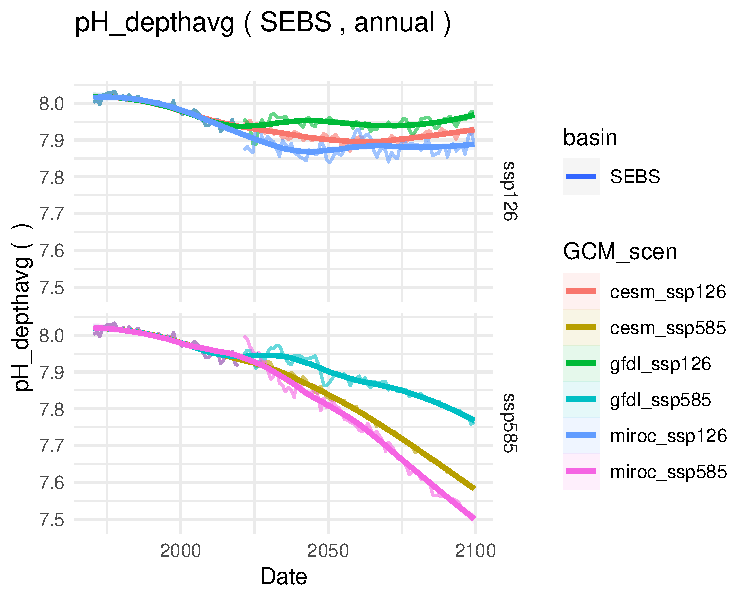
\includegraphics{ACLIM2_quickStart_files/figure-latex/ts-2} \end{center}

\begin{Shaded}
\begin{Highlighting}[]
  \CommentTok{\# plot it interactively}
\NormalTok{  plotly}\SpecialCharTok{::}\FunctionTok{ggplotly}\NormalTok{(pp)}
\end{Highlighting}
\end{Shaded}

\begin{center}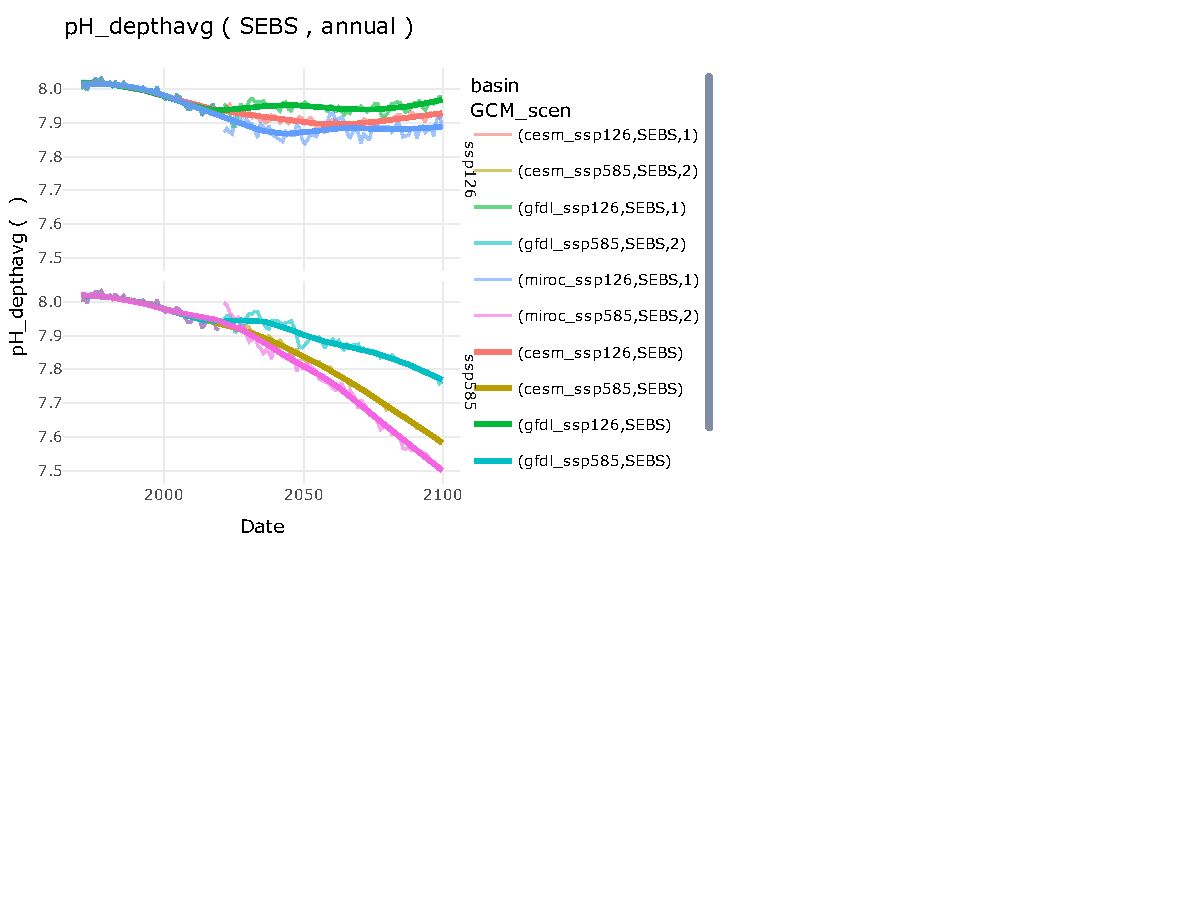
\includegraphics{ACLIM2_quickStart_files/figure-latex/unnamed-chunk-5-1} \end{center}

\hypertarget{monthly-indices-andy}{%
\subsection{monthly indices (Andy)}\label{monthly-indices-andy}}

\begin{Shaded}
\begin{Highlighting}[]
  \FunctionTok{suppressMessages}\NormalTok{(}\FunctionTok{source}\NormalTok{(}\StringTok{"R/make.R"}\NormalTok{))}
  
  \CommentTok{\# preview possible variables}
  \FunctionTok{load}\NormalTok{(}\FunctionTok{paste0}\NormalTok{(}\StringTok{"Data/out/K20P19\_CMIP6/allEBS\_means/ACLIM\_monthly\_hind\_mn.Rdata"}\NormalTok{))}
\NormalTok{  varall  }\OtherTok{\textless{}{-}} \FunctionTok{unique}\NormalTok{(ACLIM\_monthly\_hind}\SpecialCharTok{$}\NormalTok{var)}
\NormalTok{  varall}
  
\NormalTok{  scens   }\OtherTok{\textless{}{-}} \FunctionTok{c}\NormalTok{(}\StringTok{"ssp126"}\NormalTok{,}\StringTok{"ssp585"}\NormalTok{)}
\NormalTok{  GCMs    }\OtherTok{\textless{}{-}} \FunctionTok{c}\NormalTok{(}\StringTok{"miroc"}\NormalTok{,}\StringTok{"gfdl"}\NormalTok{,  }\StringTok{"cesm"}\NormalTok{ )}
\NormalTok{  varlist }\OtherTok{\textless{}{-}} \FunctionTok{c}\NormalTok{(}\StringTok{"temp\_bottom5m"}\NormalTok{,}\StringTok{"fracbelow2"}\NormalTok{,}\StringTok{"uEast\_surface5m"}\NormalTok{)}

  \CommentTok{\# get the variable you want:}
\NormalTok{  df }\OtherTok{\textless{}{-}} \FunctionTok{get\_var}\NormalTok{( }\AttributeTok{typeIN    =} \StringTok{"annual"}\NormalTok{, }
                  \AttributeTok{CMIPIN    =} \StringTok{"K20P19\_CMIP6"}\NormalTok{,}
                  \AttributeTok{plotvar   =} \StringTok{"uEast\_surface5m"}\NormalTok{,}
                  \AttributeTok{bcIN      =} \StringTok{"bias corrected"}\NormalTok{,}
                  \AttributeTok{plothist  =}\NormalTok{ F,  }\CommentTok{\# ignore the hist runs}
                  \AttributeTok{removeyr1 =}\NormalTok{ T)  }\CommentTok{\#"Remove first year of projection ( burn in)")}

\NormalTok{  df }\OtherTok{\textless{}{-}} \FunctionTok{get\_var}\NormalTok{( }\AttributeTok{typeIN    =} \StringTok{"monthly"}\NormalTok{, }
                 \AttributeTok{CMIPIN    =} \StringTok{"K20P19\_CMIP6"}\NormalTok{,}
                 \AttributeTok{monthIN   =} \DecValTok{2}\NormalTok{,}
                 \AttributeTok{plotvar   =} \StringTok{"temp\_bottom5m"}\NormalTok{,}
                 \AttributeTok{bcIN      =} \StringTok{"bias corrected"}\NormalTok{,}
                 \AttributeTok{plothist  =}\NormalTok{ F,  }\CommentTok{\# ignore the hist runs}
                 \AttributeTok{removeyr1 =}\NormalTok{ T)  }\CommentTok{\#"Remove first year of projection ( burn in)")}


  \FunctionTok{head}\NormalTok{(df}\SpecialCharTok{$}\NormalTok{dat)}
\NormalTok{  df}\SpecialCharTok{$}\NormalTok{plot}
\end{Highlighting}
\end{Shaded}

\begin{center}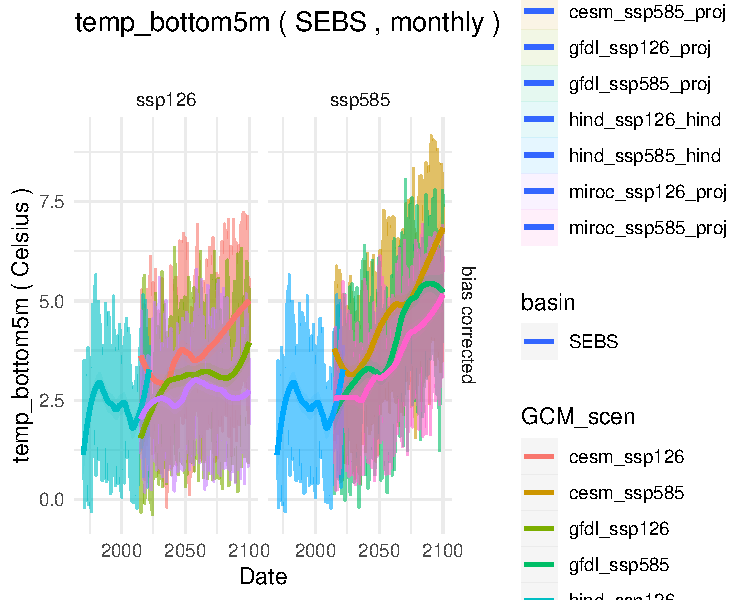
\includegraphics{ACLIM2_quickStart_files/figure-latex/ewe-1} \end{center}

\begin{Shaded}
\begin{Highlighting}[]
  \CommentTok{\# concat the hind and fut runs by removing years from projection}
\NormalTok{  maxDin }\OtherTok{\textless{}{-}} \FunctionTok{max}\NormalTok{(}\FunctionTok{as.vector}\NormalTok{(df}\SpecialCharTok{$}\NormalTok{dat}\SpecialCharTok{\%\textgreater{}\%}\NormalTok{dplyr}\SpecialCharTok{::}\FunctionTok{filter}\NormalTok{(sim\_type}\SpecialCharTok{==}\StringTok{"hind"}\NormalTok{)}\SpecialCharTok{\%\textgreater{}\%}
                            \FunctionTok{ungroup}\NormalTok{()}\SpecialCharTok{\%\textgreater{}\%}\NormalTok{dplyr}\SpecialCharTok{::}\FunctionTok{select}\NormalTok{(mnDate))[[}\DecValTok{1}\NormalTok{]])}
  
\NormalTok{  newdat }\OtherTok{\textless{}{-}} \FunctionTok{stitchTS}\NormalTok{(}\AttributeTok{dat =}\NormalTok{ df}\SpecialCharTok{$}\NormalTok{dat,}
                   \AttributeTok{maxD  =}\NormalTok{ maxDin)}
  
  \CommentTok{\# newdat has the full set of data}
  \CommentTok{\# select miroc\_ssp126}
  \FunctionTok{head}\NormalTok{(newdat}\SpecialCharTok{\%\textgreater{}\%}\NormalTok{dplyr}\SpecialCharTok{::}\FunctionTok{filter}\NormalTok{(GCM\_scen}\SpecialCharTok{==}\FunctionTok{paste0}\NormalTok{(GCMs[}\DecValTok{1}\NormalTok{],}\StringTok{"\_"}\NormalTok{,scens[}\DecValTok{1}\NormalTok{])))}
  \FunctionTok{tail}\NormalTok{(newdat}\SpecialCharTok{\%\textgreater{}\%}\NormalTok{dplyr}\SpecialCharTok{::}\FunctionTok{filter}\NormalTok{(GCM\_scen}\SpecialCharTok{==}\FunctionTok{paste0}\NormalTok{(GCMs[}\DecValTok{1}\NormalTok{],}\StringTok{"\_"}\NormalTok{,scens[}\DecValTok{1}\NormalTok{])))}


\NormalTok{  pp  }\OtherTok{\textless{}{-}} \FunctionTok{ggplot}\NormalTok{(newdat)}\SpecialCharTok{+}
            \FunctionTok{geom\_line}\NormalTok{(}\FunctionTok{aes}\NormalTok{(}\AttributeTok{x=}\NormalTok{mnDate,}\AttributeTok{y=}\NormalTok{mn\_val,}\AttributeTok{color=}\NormalTok{ GCM\_scen, }\AttributeTok{linetype =}\NormalTok{ basin),}
                      \AttributeTok{alpha =} \FloatTok{0.6}\NormalTok{,}\AttributeTok{show.legend =} \ConstantTok{FALSE}\NormalTok{)}\SpecialCharTok{+}
            \FunctionTok{geom\_smooth}\NormalTok{(}\FunctionTok{aes}\NormalTok{(}\AttributeTok{x=}\NormalTok{mnDate,}\AttributeTok{y=}\NormalTok{mn\_val,}\AttributeTok{color=}\NormalTok{ GCM\_scen,}
                            \AttributeTok{fill=}\NormalTok{GCM\_scen,}\AttributeTok{linetype =}\NormalTok{ basin),}\AttributeTok{alpha=}\FloatTok{0.1}\NormalTok{,}
                        \AttributeTok{method=}\StringTok{"loess"}\NormalTok{,}\AttributeTok{formula=}\StringTok{\textquotesingle{}y \textasciitilde{} x\textquotesingle{}}\NormalTok{,}\AttributeTok{span =}\NormalTok{ .}\DecValTok{5}\NormalTok{,}\AttributeTok{show.legend=}\NormalTok{T)}\SpecialCharTok{+}
            \FunctionTok{theme\_minimal}\NormalTok{() }\SpecialCharTok{+} 
            \FunctionTok{labs}\NormalTok{(}\AttributeTok{x=}\StringTok{"Date"}\NormalTok{,}
                   \AttributeTok{y=}\FunctionTok{paste}\NormalTok{(newdat}\SpecialCharTok{$}\NormalTok{var[}\DecValTok{1}\NormalTok{],}\StringTok{"("}\NormalTok{,newdat}\SpecialCharTok{$}\NormalTok{units[}\DecValTok{1}\NormalTok{],}\StringTok{")"}\NormalTok{),}
                   \AttributeTok{subtitle =} \StringTok{""}\NormalTok{,}
                   \AttributeTok{legend =} \StringTok{""}\NormalTok{,}
                   \AttributeTok{title =} \FunctionTok{paste}\NormalTok{(newdat}\SpecialCharTok{$}\NormalTok{var[}\DecValTok{1}\NormalTok{],}\StringTok{"("}\NormalTok{,newdat}\SpecialCharTok{$}\NormalTok{basin[}\DecValTok{1}\NormalTok{],}\StringTok{","}\NormalTok{,newdat}\SpecialCharTok{$}\NormalTok{type[}\DecValTok{1}\NormalTok{],}\StringTok{")"}\NormalTok{))}\SpecialCharTok{+}
          \FunctionTok{scale\_color\_discrete}\NormalTok{()}\SpecialCharTok{+}
          \FunctionTok{facet\_grid}\NormalTok{(scen}\SpecialCharTok{\textasciitilde{}}\NormalTok{.)}
\NormalTok{  pp}
\end{Highlighting}
\end{Shaded}

\begin{center}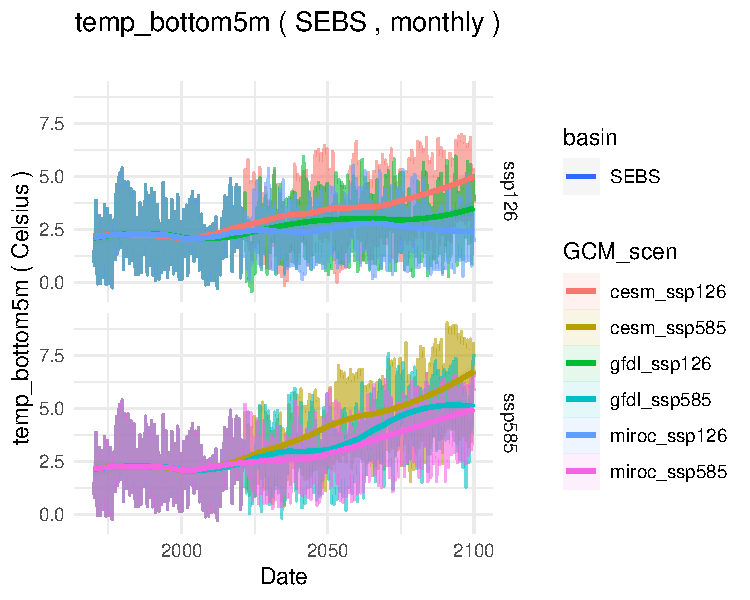
\includegraphics{ACLIM2_quickStart_files/figure-latex/ewe-2} \end{center}

\begin{Shaded}
\begin{Highlighting}[]
  \CommentTok{\# plot it interactively}
\NormalTok{  plotly}\SpecialCharTok{::}\FunctionTok{ggplotly}\NormalTok{(pp)}
\end{Highlighting}
\end{Shaded}

\begin{center}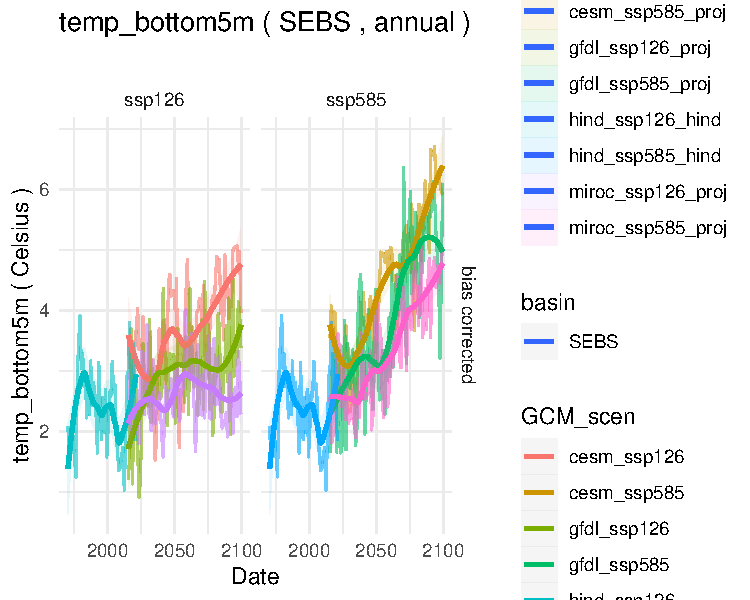
\includegraphics{ACLIM2_quickStart_files/figure-latex/unnamed-chunk-6-1} \end{center}

\hypertarget{weekly-indices-jon}{%
\subsection{weekly indices (Jon)}\label{weekly-indices-jon}}

\begin{Shaded}
\begin{Highlighting}[]
  \FunctionTok{suppressMessages}\NormalTok{(}\FunctionTok{source}\NormalTok{(}\StringTok{"R/make.R"}\NormalTok{))}
  
  \CommentTok{\# preview possible variables}
  \FunctionTok{load}\NormalTok{(}\FunctionTok{paste0}\NormalTok{(}\StringTok{"Data/out/K20P19\_CMIP6/allEBS\_means/ACLIM\_weekly\_hind\_mn.Rdata"}\NormalTok{))}
\NormalTok{  varall  }\OtherTok{\textless{}{-}} \FunctionTok{unique}\NormalTok{(ACLIM\_weekly\_hind}\SpecialCharTok{$}\NormalTok{var)}
\NormalTok{  varall}


\NormalTok{  scens   }\OtherTok{\textless{}{-}} \FunctionTok{c}\NormalTok{(}\StringTok{"ssp126"}\NormalTok{,}\StringTok{"ssp585"}\NormalTok{)}
\NormalTok{  GCMs    }\OtherTok{\textless{}{-}} \FunctionTok{c}\NormalTok{(}\StringTok{"miroc"}\NormalTok{,}\StringTok{"gfdl"}\NormalTok{,  }\StringTok{"cesm"}\NormalTok{ )}
\NormalTok{  varlist }\OtherTok{\textless{}{-}} \FunctionTok{c}\NormalTok{(}\StringTok{"temp\_bottom5m"}\NormalTok{,}\StringTok{"fracbelow2"}\NormalTok{,}\StringTok{"uEast\_surface5m"}\NormalTok{)}
  
  \CommentTok{\# get the variable you want:}
\NormalTok{  df }\OtherTok{\textless{}{-}} \FunctionTok{get\_var}\NormalTok{( }\AttributeTok{typeIN    =} \StringTok{"weekly"}\NormalTok{, }
                 \AttributeTok{plotvar   =} \StringTok{"temp\_bottom5m"}\NormalTok{,}
                 \AttributeTok{bcIN      =} \StringTok{"bias corrected"}\NormalTok{,}
                 \AttributeTok{plothist  =}\NormalTok{ F,  }\CommentTok{\# ignore the hist runs}
                 \AttributeTok{removeyr1 =}\NormalTok{ T)  }\CommentTok{\#"Remove first year of projection ( burn in)")}
  
\NormalTok{  df}\SpecialCharTok{$}\NormalTok{plot}
\end{Highlighting}
\end{Shaded}

\begin{center}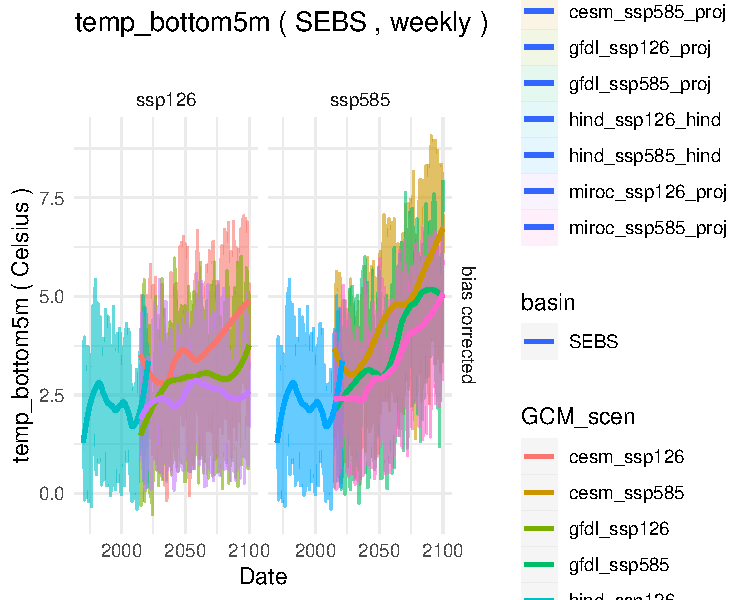
\includegraphics{ACLIM2_quickStart_files/figure-latex/sizespec-1} \end{center}

\begin{Shaded}
\begin{Highlighting}[]
  \FunctionTok{head}\NormalTok{(df}\SpecialCharTok{$}\NormalTok{dat)}
  
  \FunctionTok{ggplot}\NormalTok{(df}\SpecialCharTok{$}\NormalTok{dat}\SpecialCharTok{\%\textgreater{}\%}\FunctionTok{filter}\NormalTok{(basin}\SpecialCharTok{==}\StringTok{"SEBS"}\NormalTok{))}\SpecialCharTok{+} \FunctionTok{geom\_line}\NormalTok{(}\FunctionTok{aes}\NormalTok{(}\AttributeTok{x=}\NormalTok{jday, }\AttributeTok{y=}\NormalTok{ mn\_val, }\AttributeTok{color=}\FunctionTok{factor}\NormalTok{(year)))}\SpecialCharTok{+}\FunctionTok{facet\_wrap}\NormalTok{(GCM\_scen\_sim}\SpecialCharTok{\textasciitilde{}}\NormalTok{.)}
\end{Highlighting}
\end{Shaded}

\begin{center}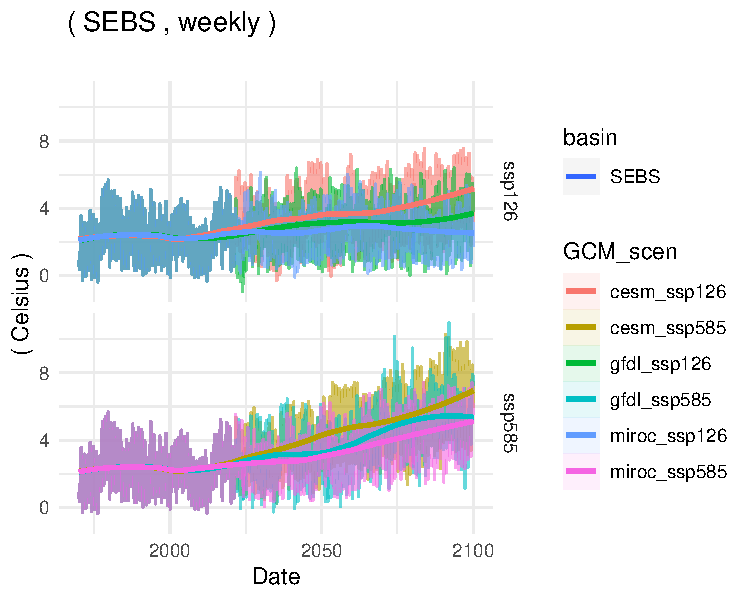
\includegraphics{ACLIM2_quickStart_files/figure-latex/sizespec-2} \end{center}

\begin{Shaded}
\begin{Highlighting}[]
  \CommentTok{\# concat the hind and fut runs by removing years from projection}
\NormalTok{  maxDin }\OtherTok{\textless{}{-}} \FunctionTok{max}\NormalTok{(}\FunctionTok{as.vector}\NormalTok{(df}\SpecialCharTok{$}\NormalTok{dat}\SpecialCharTok{\%\textgreater{}\%}\NormalTok{dplyr}\SpecialCharTok{::}\FunctionTok{filter}\NormalTok{(sim\_type}\SpecialCharTok{==}\StringTok{"hind"}\NormalTok{)}\SpecialCharTok{\%\textgreater{}\%}\NormalTok{dplyr}\SpecialCharTok{::}\FunctionTok{select}\NormalTok{(mnDate))[[}\DecValTok{1}\NormalTok{]])}
  
\NormalTok{  newdat }\OtherTok{\textless{}{-}} \FunctionTok{stitchTS}\NormalTok{(}\AttributeTok{dat =}\NormalTok{ df}\SpecialCharTok{$}\NormalTok{dat,}
                   \AttributeTok{maxD  =}\NormalTok{ maxDin)}
  
  \CommentTok{\# newdat has the full set of data}
  \CommentTok{\# select miroc\_ssp126}
  \FunctionTok{head}\NormalTok{(newdat}\SpecialCharTok{\%\textgreater{}\%}\NormalTok{dplyr}\SpecialCharTok{::}\FunctionTok{filter}\NormalTok{(GCM\_scen}\SpecialCharTok{==}\FunctionTok{paste0}\NormalTok{(GCMs[}\DecValTok{1}\NormalTok{],}\StringTok{"\_"}\NormalTok{,scens[}\DecValTok{1}\NormalTok{])))}
  
  
\NormalTok{  pp  }\OtherTok{\textless{}{-}} \FunctionTok{ggplot}\NormalTok{(newdat)}\SpecialCharTok{+}
            \FunctionTok{geom\_line}\NormalTok{(}\FunctionTok{aes}\NormalTok{(}\AttributeTok{x=}\NormalTok{mnDate,}\AttributeTok{y=}\NormalTok{mn\_val,}\AttributeTok{color=}\NormalTok{ GCM\_scen, }\AttributeTok{linetype =}\NormalTok{ basin),}
                      \AttributeTok{alpha =} \FloatTok{0.6}\NormalTok{,}\AttributeTok{show.legend =} \ConstantTok{FALSE}\NormalTok{)}\SpecialCharTok{+}
            \FunctionTok{geom\_smooth}\NormalTok{(}\FunctionTok{aes}\NormalTok{(}\AttributeTok{x=}\NormalTok{mnDate,}\AttributeTok{y=}\NormalTok{mn\_val,}\AttributeTok{color=}\NormalTok{ GCM\_scen,}
                            \AttributeTok{fill=}\NormalTok{GCM\_scen,}\AttributeTok{linetype =}\NormalTok{ basin),}\AttributeTok{alpha=}\FloatTok{0.1}\NormalTok{,}
                        \AttributeTok{method=}\StringTok{"loess"}\NormalTok{,}\AttributeTok{formula=}\StringTok{\textquotesingle{}y \textasciitilde{} x\textquotesingle{}}\NormalTok{,}\AttributeTok{span =}\NormalTok{ .}\DecValTok{5}\NormalTok{,}\AttributeTok{show.legend=}\NormalTok{T)}\SpecialCharTok{+}
            \FunctionTok{theme\_minimal}\NormalTok{() }\SpecialCharTok{+} 
            \FunctionTok{labs}\NormalTok{(}\AttributeTok{x=}\StringTok{"Date"}\NormalTok{,}
                   \AttributeTok{y=}\FunctionTok{paste}\NormalTok{(newdat}\SpecialCharTok{$}\NormalTok{var[}\DecValTok{1}\NormalTok{],}\StringTok{"("}\NormalTok{,newdat}\SpecialCharTok{$}\NormalTok{units[}\DecValTok{1}\NormalTok{],}\StringTok{")"}\NormalTok{),}
                   \AttributeTok{subtitle =} \StringTok{""}\NormalTok{,}
                   \AttributeTok{legend =} \StringTok{""}\NormalTok{,}
                   \AttributeTok{title =} \FunctionTok{paste}\NormalTok{(newdat}\SpecialCharTok{$}\NormalTok{var[}\DecValTok{1}\NormalTok{],}\StringTok{"("}\NormalTok{,newdat}\SpecialCharTok{$}\NormalTok{basin[}\DecValTok{1}\NormalTok{],}\StringTok{","}\NormalTok{,newdat}\SpecialCharTok{$}\NormalTok{type[}\DecValTok{1}\NormalTok{],}\StringTok{")"}\NormalTok{))}\SpecialCharTok{+}
          \FunctionTok{scale\_color\_discrete}\NormalTok{()}\SpecialCharTok{+}
          \FunctionTok{facet\_grid}\NormalTok{(scen}\SpecialCharTok{\textasciitilde{}}\NormalTok{.)}
  \CommentTok{\# plot it}
\NormalTok{  pp}
\end{Highlighting}
\end{Shaded}

\begin{center}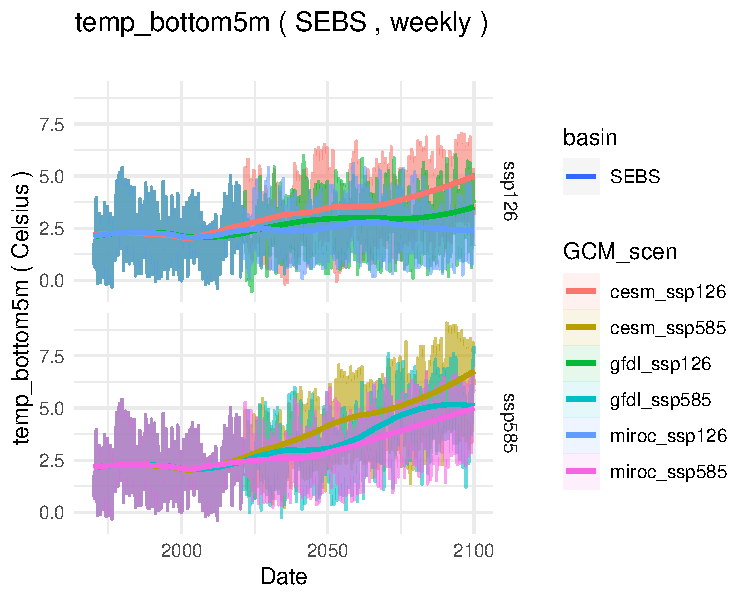
\includegraphics{ACLIM2_quickStart_files/figure-latex/sizespec-3} \end{center}

\begin{Shaded}
\begin{Highlighting}[]
  \CommentTok{\# plot it interactively}
\NormalTok{  plotly}\SpecialCharTok{::}\FunctionTok{ggplotly}\NormalTok{(pp)}
\end{Highlighting}
\end{Shaded}

\begin{center}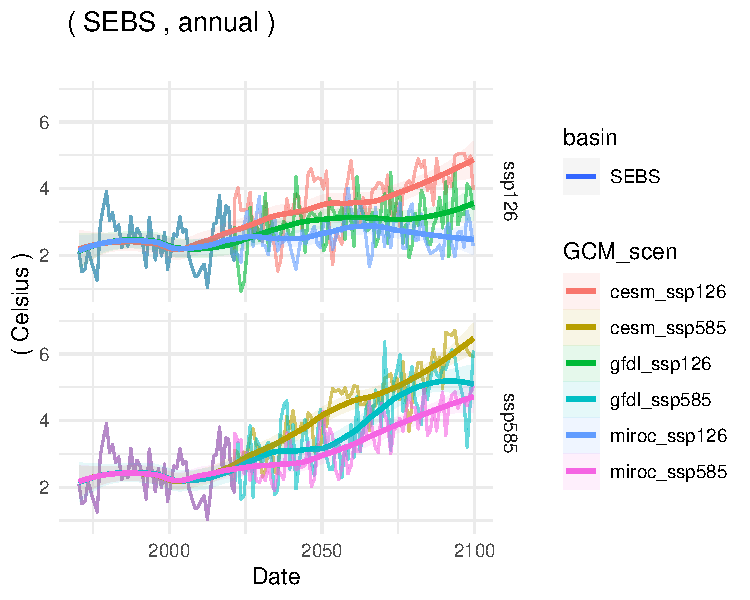
\includegraphics{ACLIM2_quickStart_files/figure-latex/unnamed-chunk-7-1} \end{center}

\begin{center}\rule{0.5\linewidth}{0.5pt}\end{center}

\hypertarget{output-to-.dat-file-admb-tmb-users}{%
\section{Output to .dat file (ADMB/ TMB
users)}\label{output-to-.dat-file-admb-tmb-users}}

For CEATTLE I create a .dat file that is read into the ADMB script. That
.dat file includes the bias corrected values (e.g., bottom temperature
in deg C) used for the bioenergetics and temperature-dependent growth
functions as well as Z-score (scaled) values used as covariates on the
recruitment function. The section below will step through that .dat file
creation for a subset of variables as well as demo chunks of ADMB code
for reading that into a ADMB based model.

\hypertarget{use-r-to-make-.dat-file-using-aclim-suite}{%
\subsection{Use R to make .dat file using ACLIM
suite}\label{use-r-to-make-.dat-file-using-aclim-suite}}

\begin{Shaded}
\begin{Highlighting}[]
  \CommentTok{\# 1 {-}{-} create .dat filename \& path}
  \CommentTok{\# 2 {-}{-} rescale (Z{-}score) data and get variables}
  \CommentTok{\# 3 {-}{-} write data to hind .dat file}
  \CommentTok{\# 3 {-}{-} write data to fut  .dat file}
  
  \CommentTok{\# 1 {-}{-} create .dat filename \& path}
  \CommentTok{\# {-}{-}{-}{-}{-}{-}{-}{-}{-}{-}{-}{-}{-}{-}{-}{-}{-}{-}{-}{-}{-}{-}{-}{-}{-}{-}{-}{-}{-}{-}{-}{-}{-}{-}{-}{-}{-}}
  \FunctionTok{suppressMessages}\NormalTok{(}\FunctionTok{source}\NormalTok{(}\StringTok{"R/make.R"}\NormalTok{))}

  
  \CommentTok{\# switches }
\NormalTok{    thisYr }\OtherTok{\textless{}{-}} \FunctionTok{format}\NormalTok{(}\FunctionTok{Sys.time}\NormalTok{(), }\StringTok{"\%Y"}\NormalTok{)}
\NormalTok{    today  }\OtherTok{\textless{}{-}} \FunctionTok{format}\NormalTok{(}\FunctionTok{Sys.time}\NormalTok{(), }\StringTok{"\%b \%d, \%Y"}\NormalTok{)}
\NormalTok{    lastyr\_hind }\OtherTok{\textless{}{-}} \FunctionTok{as.numeric}\NormalTok{(thisYr)  }\CommentTok{\#2021}
\NormalTok{    hind\_yrs    }\OtherTok{\textless{}{-}} \DecValTok{1979}\SpecialCharTok{:}\NormalTok{lastyr\_hind   }\CommentTok{\# define the years of your estimation model}
\NormalTok{    fut\_yrs     }\OtherTok{\textless{}{-}}\NormalTok{ (lastyr\_hind}\SpecialCharTok{+}\DecValTok{1}\NormalTok{)}\SpecialCharTok{:}\DecValTok{2100}   \CommentTok{\# define the years of your projections}
\NormalTok{    log\_adj     }\OtherTok{\textless{}{-}} \FloatTok{1e{-}4}
\NormalTok{    plotbasin   }\OtherTok{\textless{}{-}} \StringTok{"SEBS"}  
  
  \CommentTok{\# Define the name for the .dat file}
\NormalTok{    file.name   }\OtherTok{\textless{}{-}} \StringTok{"ACLIM2\_CMIP6\_short"}
\NormalTok{    fn          }\OtherTok{\textless{}{-}} \FunctionTok{paste}\NormalTok{(file.name,}\StringTok{"\_bcs.dat"}\NormalTok{,}\AttributeTok{sep=}\StringTok{""}\NormalTok{)}
\NormalTok{    archive\_old }\OtherTok{\textless{}{-}}\NormalTok{ T  }\CommentTok{\# Archive the older version of the .dat file?}
\NormalTok{    normlist    }\OtherTok{\textless{}{-}} \FunctionTok{read.csv}\NormalTok{(}\AttributeTok{file=}\FunctionTok{file.path}\NormalTok{(Rdata\_path,}\StringTok{"../normlist.csv"}\NormalTok{))}
    
\NormalTok{    outpath     }\OtherTok{\textless{}{-}} \StringTok{"Data/out/ADMB\_datfiles"}
    \ControlFlowTok{if}\NormalTok{(}\SpecialCharTok{!}\FunctionTok{dir.exists}\NormalTok{(outpath)) }\FunctionTok{dir.create}\NormalTok{(outpath)}
    
  \CommentTok{\# define hind and fut data files}
\NormalTok{    fndat\_hind  }\OtherTok{\textless{}{-}} \FunctionTok{file.path}\NormalTok{(outpath,}\FunctionTok{paste}\NormalTok{(}\StringTok{"KKHhind\_"}\NormalTok{,fn,}\AttributeTok{sep=}\StringTok{""}\NormalTok{))}
\NormalTok{    fndat\_fut   }\OtherTok{\textless{}{-}} \FunctionTok{file.path}\NormalTok{(outpath,}\FunctionTok{paste}\NormalTok{(}\StringTok{"KKHfut\_"}\NormalTok{,fn,}\AttributeTok{sep=}\StringTok{""}\NormalTok{))}
\NormalTok{    fndat\_hind2 }\OtherTok{\textless{}{-}} \FunctionTok{file.path}\NormalTok{(outpath,}\FunctionTok{paste}\NormalTok{(}\StringTok{"hind\_"}\NormalTok{,fn,}\AttributeTok{sep=}\StringTok{""}\NormalTok{))}
\NormalTok{    fndat\_fut2  }\OtherTok{\textless{}{-}} \FunctionTok{file.path}\NormalTok{(outpath,}\FunctionTok{paste}\NormalTok{(}\StringTok{"fut\_"}\NormalTok{,fn,}\AttributeTok{sep=}\StringTok{""}\NormalTok{))}
    
    \CommentTok{\# create and archive .dat files}
\NormalTok{      outfile    }\OtherTok{\textless{}{-}}\NormalTok{ fndat\_fut}
    \ControlFlowTok{if}\NormalTok{(}\FunctionTok{file.exists}\NormalTok{(outfile)}\SpecialCharTok{\&}\NormalTok{archive\_old)\{   }
        \CommentTok{\# archive older version}
\NormalTok{            archivefl }\OtherTok{\textless{}{-}} \FunctionTok{paste0}\NormalTok{(}\FunctionTok{substr}\NormalTok{(outfile,}\AttributeTok{start=}\DecValTok{1}\NormalTok{,}\AttributeTok{stop=}\FunctionTok{nchar}\NormalTok{(outfile)}\SpecialCharTok{{-}}\DecValTok{4}\NormalTok{),}
                            \FunctionTok{format}\NormalTok{(}\FunctionTok{Sys.time}\NormalTok{(), }\StringTok{"\%Y\%m\%d\_\%H\%M\%S"}\NormalTok{),}\StringTok{".dat"}\NormalTok{)}
            \FunctionTok{file.rename}\NormalTok{(outfile, archivefl)}
            \CommentTok{\#file.remove(outfile)}
\NormalTok{    \}}
    
    \FunctionTok{file.create}\NormalTok{(outfile)}
\NormalTok{    outfile  }\OtherTok{\textless{}{-}}\NormalTok{ fndat\_hind}
    \ControlFlowTok{if}\NormalTok{(}\FunctionTok{file.exists}\NormalTok{(outfile)}\SpecialCharTok{\&}\NormalTok{archive\_old)\{   }
        \CommentTok{\# archive older version}
\NormalTok{            archivefl }\OtherTok{\textless{}{-}} \FunctionTok{paste0}\NormalTok{(}\FunctionTok{substr}\NormalTok{(outfile,}\AttributeTok{start=}\DecValTok{1}\NormalTok{,}\AttributeTok{stop=}\FunctionTok{nchar}\NormalTok{(outfile)}\SpecialCharTok{{-}}\DecValTok{4}\NormalTok{),}
                            \FunctionTok{format}\NormalTok{(}\FunctionTok{Sys.time}\NormalTok{(), }\StringTok{"\%Y\%m\%d\_\%H\%M\%S"}\NormalTok{),}\StringTok{".dat"}\NormalTok{)}
            \FunctionTok{file.rename}\NormalTok{(outfile, archivefl)}
            \CommentTok{\#file.remove(outfile)}
\NormalTok{    \}}
    
    \FunctionTok{file.create}\NormalTok{(outfile)}

    \CommentTok{\# 2 {-}{-} rescale (Z{-}score) data and get variables}
    \CommentTok{\# CMIPS \textless{}{-} c("K20P19\_CMIP6","K20P19\_CMIP5")}
    \CommentTok{\# CMIPS \textless{}{-} c("K20P19\_CMIP6\_C")}
    
\NormalTok{    CMIPS }\OtherTok{\textless{}{-}} \FunctionTok{c}\NormalTok{(}\StringTok{"K20P19\_CMIP6"}\NormalTok{,}\StringTok{"K20P19\_CMIP5"}\NormalTok{)}
    
    \CommentTok{\# preview possible variables}
    \FunctionTok{load}\NormalTok{(}\FunctionTok{paste0}\NormalTok{(}\StringTok{"Data/out/"}\NormalTok{,CMIPS[}\DecValTok{1}\NormalTok{],}\StringTok{"/allEBS\_means/ACLIM\_annual\_hind\_mn.Rdata"}\NormalTok{))}
\NormalTok{    varall  }\OtherTok{\textless{}{-}} \FunctionTok{unique}\NormalTok{(ACLIM\_annual\_hind}\SpecialCharTok{$}\NormalTok{var)}
\NormalTok{    varall}
    
    \CommentTok{\# get each variable, convert to TS and rbind}
    
    \ControlFlowTok{for}\NormalTok{(c }\ControlFlowTok{in} \DecValTok{1}\SpecialCharTok{:}\FunctionTok{length}\NormalTok{(CMIPS))\{}

      \CommentTok{\# first for annual mean values:}
\NormalTok{        varlist }\OtherTok{\textless{}{-}} \FunctionTok{c}\NormalTok{(}\StringTok{"largeZoop\_integrated"}\NormalTok{,}\StringTok{"fracbelow2"}\NormalTok{,}
                     \StringTok{"temp\_bottom5m"}\NormalTok{,}\StringTok{"temp\_surface5m"}\NormalTok{,}\StringTok{"pH\_depthavg"}\NormalTok{)}
\NormalTok{        varlist }\OtherTok{\textless{}{-}} \FunctionTok{c}\NormalTok{(}\StringTok{"largeZoop\_integrated"}\NormalTok{,}\StringTok{"fracbelow2"}\NormalTok{,}
                     \StringTok{"temp\_bottom5m"}\NormalTok{,}\StringTok{"temp\_surface5m"}\NormalTok{,}\StringTok{"pH\_depthavg"}\NormalTok{)}
        
      \CommentTok{\# norm\_sub \textless{}{-} normlist\%\textgreater{}\%filter(var\%in\%varlist)}
\NormalTok{        typeIN }\OtherTok{\textless{}{-}} \StringTok{"annual"}
        \FunctionTok{load}\NormalTok{(}\FunctionTok{paste0}\NormalTok{(}\StringTok{"Data/out/"}\NormalTok{,CMIPS[c],}\StringTok{"/allEBS\_means/ACLIM\_"}\NormalTok{,typeIN,}\StringTok{"\_hind\_mn.Rdata"}\NormalTok{))}
        \FunctionTok{load}\NormalTok{(}\FunctionTok{paste0}\NormalTok{(}\StringTok{"Data/out/"}\NormalTok{,CMIPS[c],}\StringTok{"/allEBS\_means/ACLIM\_"}\NormalTok{,typeIN,}\StringTok{"\_fut\_mn.Rdata"}\NormalTok{))}
        \FunctionTok{eval}\NormalTok{(}\FunctionTok{parse}\NormalTok{(}\AttributeTok{text =} \FunctionTok{paste0}\NormalTok{(}\StringTok{"dhind \textless{}{-} ACLIM\_"}\NormalTok{,typeIN,}\StringTok{"\_hind"}\NormalTok{)))}
        \FunctionTok{eval}\NormalTok{(}\FunctionTok{parse}\NormalTok{(}\AttributeTok{text =} \FunctionTok{paste0}\NormalTok{(}\StringTok{"dfut  \textless{}{-} ACLIM\_"}\NormalTok{,typeIN,}\StringTok{"\_fut"}\NormalTok{)))}
       
      \CommentTok{\# Z{-}score the data}
\NormalTok{       tmphind    }\OtherTok{\textless{}{-}} \FunctionTok{suppressWarnings}\NormalTok{(dhind}\SpecialCharTok{\%\textgreater{}\%}
\NormalTok{         dplyr}\SpecialCharTok{::}\FunctionTok{filter}\NormalTok{(var}\SpecialCharTok{\%in\%}\NormalTok{varlist,basin}\SpecialCharTok{==}\NormalTok{plotbasin,year}\SpecialCharTok{\%in\%}\NormalTok{hind\_yrs)}\SpecialCharTok{\%\textgreater{}\%}
       \CommentTok{\# dplyr::left\_join(normlist,by=c("var"="var"))\%\textgreater{}\%}
\NormalTok{         dplyr}\SpecialCharTok{::}\FunctionTok{select}\NormalTok{(var,basin,year,mnDate,mn\_val, }
\NormalTok{                       mnVal\_hind,sdVal\_hind, sim,gcmcmip,}
\NormalTok{                       CMIP,GCM,scen,sim\_type ,units,long\_name)}\SpecialCharTok{\%\textgreater{}\%}
\NormalTok{         dplyr}\SpecialCharTok{::}\FunctionTok{mutate}\NormalTok{(}\AttributeTok{bc =} \StringTok{"bias corrected"}\NormalTok{,}
                       \AttributeTok{GCM\_scen =} \FunctionTok{paste0}\NormalTok{(GCM,}\StringTok{"\_"}\NormalTok{,scen),}
                       \AttributeTok{mn\_val\_scaled =}\NormalTok{  (mn\_val}\SpecialCharTok{{-}}\NormalTok{mnVal\_hind )}\SpecialCharTok{/}\NormalTok{sdVal\_hind ))}
       
\NormalTok{       tmpfut    }\OtherTok{\textless{}{-}}  \FunctionTok{suppressWarnings}\NormalTok{(dfut}\SpecialCharTok{\%\textgreater{}\%}
\NormalTok{         dplyr}\SpecialCharTok{::}\FunctionTok{filter}\NormalTok{(var}\SpecialCharTok{\%in\%}\NormalTok{varlist,basin}\SpecialCharTok{==}\NormalTok{plotbasin,year}\SpecialCharTok{\%in\%}\NormalTok{fut\_yrs)}\SpecialCharTok{\%\textgreater{}\%}
\NormalTok{         dplyr}\SpecialCharTok{::}\FunctionTok{select}\NormalTok{(var,basin,year,mnDate,mn\_val, val\_biascorrected, }
\NormalTok{                       mnVal\_hind,sdVal\_hind, sim,gcmcmip,}
\NormalTok{                       CMIP,GCM,scen,sim\_type ,units,long\_name)}\SpecialCharTok{\%\textgreater{}\%}         
\NormalTok{         dplyr}\SpecialCharTok{::}\FunctionTok{mutate}\NormalTok{(}\AttributeTok{bc =} \StringTok{"bias corrected"}\NormalTok{,}
                       \AttributeTok{GCM\_scen =} \FunctionTok{paste0}\NormalTok{(GCM,}\StringTok{"\_"}\NormalTok{,scen),}
                       \AttributeTok{mn\_val\_scaled =}\NormalTok{  (val\_biascorrected}\SpecialCharTok{{-}}\NormalTok{mnVal\_hind )}\SpecialCharTok{/}\NormalTok{sdVal\_hind))}
       
       \ControlFlowTok{if}\NormalTok{(}\DecValTok{1}\SpecialCharTok{==}\DecValTok{2}\NormalTok{)\{}
         
\NormalTok{          hind2 }\OtherTok{\textless{}{-}} \FunctionTok{rbind}\NormalTok{(}
\NormalTok{            tmphind}\SpecialCharTok{\%\textgreater{}\%}\FunctionTok{select}\NormalTok{(year,var, mn\_val, scen, GCM)}\SpecialCharTok{\%\textgreater{}\%}\FunctionTok{mutate}\NormalTok{(}\AttributeTok{type =} \StringTok{"a) raw"}\NormalTok{),}
\NormalTok{            tmphind}\SpecialCharTok{\%\textgreater{}\%}\FunctionTok{select}\NormalTok{(year,var, mn\_val, scen, GCM)}\SpecialCharTok{\%\textgreater{}\%}\FunctionTok{mutate}\NormalTok{(}\AttributeTok{type =} \StringTok{"b) bias corrected"}\NormalTok{),}
\NormalTok{            tmphind}\SpecialCharTok{\%\textgreater{}\%}\FunctionTok{select}\NormalTok{(year,var, mn\_val\_scaled, scen, GCM)}\SpecialCharTok{\%\textgreater{}\%}
              \FunctionTok{rename}\NormalTok{(}\AttributeTok{mn\_val =}\NormalTok{ mn\_val\_scaled)}\SpecialCharTok{\%\textgreater{}\%}\FunctionTok{mutate}\NormalTok{(}\AttributeTok{type =} \StringTok{"c) bias corrected \&  scaled"}\NormalTok{))}
\NormalTok{          fut2 }\OtherTok{\textless{}{-}} \FunctionTok{rbind}\NormalTok{(}
\NormalTok{            tmpfut}\SpecialCharTok{\%\textgreater{}\%}\FunctionTok{select}\NormalTok{(year,var, mn\_val, scen, GCM)}\SpecialCharTok{\%\textgreater{}\%}\FunctionTok{mutate}\NormalTok{(}\AttributeTok{type =} \StringTok{"a) raw"}\NormalTok{),}
\NormalTok{            tmpfut}\SpecialCharTok{\%\textgreater{}\%}\FunctionTok{select}\NormalTok{(year,var, val\_biascorrected, scen, GCM)}\SpecialCharTok{\%\textgreater{}\%}
              \FunctionTok{rename}\NormalTok{(}\AttributeTok{mn\_val =}\NormalTok{ val\_biascorrected)}\SpecialCharTok{\%\textgreater{}\%}\FunctionTok{mutate}\NormalTok{(}\AttributeTok{type =} \StringTok{"b) bias corrected"}\NormalTok{),}
\NormalTok{            tmpfut}\SpecialCharTok{\%\textgreater{}\%}\FunctionTok{select}\NormalTok{(year,var, mn\_val\_scaled, scen, GCM)}\SpecialCharTok{\%\textgreater{}\%}
              \FunctionTok{rename}\NormalTok{(}\AttributeTok{mn\_val =}\NormalTok{ mn\_val\_scaled)}\SpecialCharTok{\%\textgreater{}\%}\FunctionTok{mutate}\NormalTok{(}\AttributeTok{type =} \StringTok{"c) bias corrected \&  scaled"}\NormalTok{))}
         
\NormalTok{          pcompare }\OtherTok{\textless{}{-}} \FunctionTok{ggplot}\NormalTok{(hind2)}\SpecialCharTok{+}
           \FunctionTok{geom\_line}\NormalTok{(}\FunctionTok{aes}\NormalTok{(}\AttributeTok{x=}\NormalTok{year,}\AttributeTok{y=}\NormalTok{mn\_val ,}\AttributeTok{color=}\NormalTok{scen),}\AttributeTok{size=}\NormalTok{.}\DecValTok{8}\NormalTok{)}\SpecialCharTok{+}
           \FunctionTok{geom\_line}\NormalTok{(}\AttributeTok{data =}\NormalTok{fut2,}\FunctionTok{aes}\NormalTok{(}\AttributeTok{x=}\NormalTok{year,}\AttributeTok{y=}\NormalTok{mn\_val,}\AttributeTok{color=}\NormalTok{scen, }\AttributeTok{linetype =}\NormalTok{ GCM ),}\AttributeTok{size=}\NormalTok{.}\DecValTok{8}\NormalTok{)}\SpecialCharTok{+}
           \FunctionTok{facet\_wrap}\NormalTok{(var}\SpecialCharTok{\textasciitilde{}}\NormalTok{type,}\AttributeTok{scales=}\StringTok{"free\_y"}\NormalTok{,}\AttributeTok{nrow =}\FunctionTok{length}\NormalTok{(varlist))}\SpecialCharTok{+}\FunctionTok{theme\_minimal}\NormalTok{()}
\NormalTok{          pcompare}
          
\NormalTok{          sclr }\OtherTok{\textless{}{-}}\FloatTok{1.2}
          \FunctionTok{png}\NormalTok{(}\StringTok{"Figs/compare\_scaled2raw\_2022.png"}\NormalTok{, }
              \AttributeTok{width =}\DecValTok{6}\SpecialCharTok{*}\NormalTok{sclr, }\AttributeTok{height =}\DecValTok{9}\SpecialCharTok{*}\NormalTok{sclr, }\AttributeTok{units =} \StringTok{"in"}\NormalTok{,}\AttributeTok{res =} \DecValTok{150}\NormalTok{)}
          \FunctionTok{print}\NormalTok{( pcompare)  }\CommentTok{\# hypoxic (O2\textless{}70mmol m−3) or suboxic (O2\textless{}5mmol m−3),}
          \FunctionTok{dev.off}\NormalTok{()}
      
          
\NormalTok{       \}}
       
      \CommentTok{\# now for seasonal mean values:}
       
\NormalTok{      typeIN    }\OtherTok{\textless{}{-}} \StringTok{"seasonal"}
\NormalTok{      seasonsIN }\OtherTok{\textless{}{-}} \FunctionTok{unique}\NormalTok{(seasons}\SpecialCharTok{$}\NormalTok{season)}
      
      \FunctionTok{load}\NormalTok{(}\FunctionTok{paste0}\NormalTok{(}\StringTok{"Data/out/"}\NormalTok{,CMIPS[c],}\StringTok{"/allEBS\_means/ACLIM\_"}\NormalTok{,typeIN,}\StringTok{"\_hind\_mn.Rdata"}\NormalTok{))}
      \FunctionTok{load}\NormalTok{(}\FunctionTok{paste0}\NormalTok{(}\StringTok{"Data/out/"}\NormalTok{,CMIPS[c],}\StringTok{"/allEBS\_means/ACLIM\_"}\NormalTok{,typeIN,}\StringTok{"\_fut\_mn.Rdata"}\NormalTok{))}
      \FunctionTok{eval}\NormalTok{(}\FunctionTok{parse}\NormalTok{(}\AttributeTok{text =} \FunctionTok{paste0}\NormalTok{(}\StringTok{"dhind \textless{}{-} ACLIM\_"}\NormalTok{,typeIN,}\StringTok{"\_hind"}\NormalTok{)))}
      \FunctionTok{eval}\NormalTok{(}\FunctionTok{parse}\NormalTok{(}\AttributeTok{text =} \FunctionTok{paste0}\NormalTok{(}\StringTok{"dfut  \textless{}{-} ACLIM\_"}\NormalTok{,typeIN,}\StringTok{"\_fut"}\NormalTok{)))}
      
      
       \CommentTok{\# z{-}score the data}
\NormalTok{       tmphind2    }\OtherTok{\textless{}{-}}\NormalTok{ dhind}\SpecialCharTok{\%\textgreater{}\%}
\NormalTok{         dplyr}\SpecialCharTok{::}\FunctionTok{filter}\NormalTok{(var}\SpecialCharTok{\%in\%}\NormalTok{varlist,basin}\SpecialCharTok{==}\NormalTok{plotbasin,}
\NormalTok{                       year}\SpecialCharTok{\%in\%}\NormalTok{hind\_yrs,}
\NormalTok{                       season}\SpecialCharTok{\%in\%}\NormalTok{seasonsIN)}\SpecialCharTok{\%\textgreater{}\%}
\NormalTok{         dplyr}\SpecialCharTok{::}\FunctionTok{mutate}\NormalTok{(}\AttributeTok{var =} \FunctionTok{paste0}\NormalTok{(var,}\StringTok{"\_"}\NormalTok{,season))}\SpecialCharTok{\%\textgreater{}\%}
\NormalTok{          dplyr}\SpecialCharTok{::}\FunctionTok{select}\NormalTok{(var,basin,year,mnDate,mn\_val, }
\NormalTok{                       mnVal\_hind,sdVal\_hind, sim,gcmcmip,}
\NormalTok{                       CMIP,GCM,scen,sim\_type ,units,long\_name)}\SpecialCharTok{\%\textgreater{}\%}
\NormalTok{         dplyr}\SpecialCharTok{::}\FunctionTok{mutate}\NormalTok{(}\AttributeTok{bc =} \StringTok{"bias corrected"}\NormalTok{,}
                       \AttributeTok{GCM\_scen =} \FunctionTok{paste0}\NormalTok{(GCM,}\StringTok{"\_"}\NormalTok{,scen),}
                       \AttributeTok{mn\_val\_scaled =}\NormalTok{ (mn\_val}\SpecialCharTok{{-}}\NormalTok{mnVal\_hind )}\SpecialCharTok{/}\NormalTok{sdVal\_hind)}
       
\NormalTok{       tmpfut2    }\OtherTok{\textless{}{-}}\NormalTok{ dfut}\SpecialCharTok{\%\textgreater{}\%}
\NormalTok{         dplyr}\SpecialCharTok{::}\FunctionTok{filter}\NormalTok{(var}\SpecialCharTok{\%in\%}\NormalTok{varlist,basin}\SpecialCharTok{==}\NormalTok{plotbasin,}
\NormalTok{                       year}\SpecialCharTok{\%in\%}\NormalTok{fut\_yrs,season}\SpecialCharTok{\%in\%}\NormalTok{seasonsIN)}\SpecialCharTok{\%\textgreater{}\%}
\NormalTok{         dplyr}\SpecialCharTok{::}\FunctionTok{mutate}\NormalTok{(}\AttributeTok{var =} \FunctionTok{paste0}\NormalTok{(var,}\StringTok{"\_"}\NormalTok{,season))}\SpecialCharTok{\%\textgreater{}\%}
\NormalTok{         dplyr}\SpecialCharTok{::}\FunctionTok{select}\NormalTok{(var,basin,year,mnDate,mn\_val, val\_biascorrected, }
\NormalTok{                       mnVal\_hind,sdVal\_hind, sim,gcmcmip,}
\NormalTok{                       CMIP,GCM,scen,sim\_type ,units,long\_name)}\SpecialCharTok{\%\textgreater{}\%}
\NormalTok{         dplyr}\SpecialCharTok{::}\FunctionTok{mutate}\NormalTok{(}\AttributeTok{bc =} \StringTok{"bias corrected"}\NormalTok{,}
                       \AttributeTok{GCM\_scen =} \FunctionTok{paste0}\NormalTok{(GCM,}\StringTok{"\_"}\NormalTok{,scen),}
                       \AttributeTok{mn\_val\_scaled =}\NormalTok{ (val\_biascorrected}\SpecialCharTok{{-}}\NormalTok{mnVal\_hind )}\SpecialCharTok{/}
\NormalTok{                         (sdVal\_hind))}
       
       \ControlFlowTok{if}\NormalTok{(c }\SpecialCharTok{==}\DecValTok{1}\NormalTok{)\{}
\NormalTok{          hind  }\OtherTok{\textless{}{-}} \FunctionTok{rbind}\NormalTok{(tmphind,tmphind2)}
\NormalTok{          fut   }\OtherTok{\textless{}{-}} \FunctionTok{rbind}\NormalTok{(tmpfut,tmpfut2)}
\NormalTok{       \}}\ControlFlowTok{else}\NormalTok{\{}
\NormalTok{          hind  }\OtherTok{\textless{}{-}} \FunctionTok{rbind}\NormalTok{(hind,tmphind,tmphind2)}
\NormalTok{          fut   }\OtherTok{\textless{}{-}} \FunctionTok{rbind}\NormalTok{(fut,tmpfut,tmpfut2)}
\NormalTok{       \}}
       
\NormalTok{    \}}
    
    \ControlFlowTok{if}\NormalTok{(}\DecValTok{1}\SpecialCharTok{==}\DecValTok{2}\NormalTok{)\{}
         
\NormalTok{          hind2 }\OtherTok{\textless{}{-}} \FunctionTok{rbind}\NormalTok{(}
\NormalTok{            hind}\SpecialCharTok{\%\textgreater{}\%}\FunctionTok{select}\NormalTok{(year,var, mn\_val, scen, GCM)}\SpecialCharTok{\%\textgreater{}\%}\FunctionTok{mutate}\NormalTok{(}\AttributeTok{type =} \StringTok{"a) raw"}\NormalTok{),}
\NormalTok{            hind}\SpecialCharTok{\%\textgreater{}\%}\FunctionTok{select}\NormalTok{(year,var, mn\_val, scen, GCM)}\SpecialCharTok{\%\textgreater{}\%}\FunctionTok{mutate}\NormalTok{(}\AttributeTok{type =} \StringTok{"b) bias corrected"}\NormalTok{),}
\NormalTok{            hind}\SpecialCharTok{\%\textgreater{}\%}\FunctionTok{select}\NormalTok{(year,var, mn\_val\_scaled, scen, GCM)}\SpecialCharTok{\%\textgreater{}\%}
              \FunctionTok{rename}\NormalTok{(}\AttributeTok{mn\_val =}\NormalTok{ mn\_val\_scaled)}\SpecialCharTok{\%\textgreater{}\%}\FunctionTok{mutate}\NormalTok{(}\AttributeTok{type =} \StringTok{"c) bias corrected \&  scaled"}\NormalTok{))}
          
\NormalTok{          fut2 }\OtherTok{\textless{}{-}} \FunctionTok{rbind}\NormalTok{(}
\NormalTok{            fut}\SpecialCharTok{\%\textgreater{}\%}\FunctionTok{select}\NormalTok{(year,var, mn\_val, scen, GCM)}\SpecialCharTok{\%\textgreater{}\%}\FunctionTok{mutate}\NormalTok{(}\AttributeTok{type =} \StringTok{"a) raw"}\NormalTok{),}
\NormalTok{            fut}\SpecialCharTok{\%\textgreater{}\%}\FunctionTok{select}\NormalTok{(year,var, val\_biascorrected, scen, GCM)}\SpecialCharTok{\%\textgreater{}\%}
              \FunctionTok{rename}\NormalTok{(}\AttributeTok{mn\_val =}\NormalTok{ val\_biascorrected)}\SpecialCharTok{\%\textgreater{}\%}\FunctionTok{mutate}\NormalTok{(}\AttributeTok{type =} \StringTok{"b) bias corrected"}\NormalTok{),}
\NormalTok{            fut}\SpecialCharTok{\%\textgreater{}\%}\FunctionTok{select}\NormalTok{(year,var, mn\_val\_scaled, scen, GCM)}\SpecialCharTok{\%\textgreater{}\%}
              \FunctionTok{rename}\NormalTok{(}\AttributeTok{mn\_val =}\NormalTok{ mn\_val\_scaled)}\SpecialCharTok{\%\textgreater{}\%}\FunctionTok{mutate}\NormalTok{(}\AttributeTok{type =} \StringTok{"c) bias corrected \&  scaled"}\NormalTok{))}
         
\NormalTok{          pcompare2 }\OtherTok{\textless{}{-}} \FunctionTok{ggplot}\NormalTok{(hind2[}\FunctionTok{grep}\NormalTok{(}\StringTok{"largeZoop"}\NormalTok{,}\AttributeTok{x=}\NormalTok{hind2}\SpecialCharTok{$}\NormalTok{var),])}\SpecialCharTok{+}
            \FunctionTok{geom\_line}\NormalTok{(}\FunctionTok{aes}\NormalTok{(}\AttributeTok{x=}\NormalTok{year,}\AttributeTok{y=}\NormalTok{mn\_val ,}\AttributeTok{color=}\NormalTok{scen),}\AttributeTok{size=}\NormalTok{.}\DecValTok{8}\NormalTok{)}\SpecialCharTok{+}
            \FunctionTok{geom\_line}\NormalTok{(}\AttributeTok{data =}\NormalTok{fut2[}\FunctionTok{grep}\NormalTok{(}\StringTok{"largeZoop"}\NormalTok{,}\AttributeTok{x=}\NormalTok{fut2}\SpecialCharTok{$}\NormalTok{var),],}
                      \FunctionTok{aes}\NormalTok{(}\AttributeTok{x=}\NormalTok{year,}\AttributeTok{y=}\NormalTok{mn\_val,}\AttributeTok{color=}\NormalTok{scen, }\AttributeTok{linetype =}\NormalTok{ GCM ),}\AttributeTok{size=}\NormalTok{.}\DecValTok{8}\NormalTok{)}\SpecialCharTok{+}
            \FunctionTok{facet\_wrap}\NormalTok{(var}\SpecialCharTok{\textasciitilde{}}\NormalTok{type,}\AttributeTok{scales=}\StringTok{"free\_y"}\NormalTok{,}\AttributeTok{ncol =}\DecValTok{3}\NormalTok{)}\SpecialCharTok{+}\FunctionTok{theme\_minimal}\NormalTok{()}
\NormalTok{          pcompare2}
          
\NormalTok{          sclr }\OtherTok{\textless{}{-}}\FloatTok{1.4}
          \FunctionTok{png}\NormalTok{(}\StringTok{"Figs/compare\_scaled2raw\_2022\_all.png"}\NormalTok{, }
              \AttributeTok{width =}\DecValTok{6}\SpecialCharTok{*}\NormalTok{sclr, }\AttributeTok{height =}\DecValTok{9}\SpecialCharTok{*}\NormalTok{sclr, }\AttributeTok{units =} \StringTok{"in"}\NormalTok{,}\AttributeTok{res =} \DecValTok{150}\NormalTok{)}
          \FunctionTok{print}\NormalTok{( pcompare2)  }\CommentTok{\# hypoxic (O2\textless{}70mmol m−3) or suboxic (O2\textless{}5mmol m−3),}
          \FunctionTok{dev.off}\NormalTok{()}
      
          
\NormalTok{    \}}
    
    
    
      \CommentTok{\# plot the data}
\NormalTok{       p }\OtherTok{\textless{}{-}} \FunctionTok{ggplot}\NormalTok{(hind)}\SpecialCharTok{+}
         \FunctionTok{geom\_line}\NormalTok{(}\FunctionTok{aes}\NormalTok{(}\AttributeTok{x=}\NormalTok{mnDate,}\AttributeTok{y=}\NormalTok{mn\_val,}\AttributeTok{color=}\NormalTok{GCM\_scen))}\SpecialCharTok{+}
         \FunctionTok{geom\_line}\NormalTok{(}\AttributeTok{data=}\NormalTok{fut,}\FunctionTok{aes}\NormalTok{(}\AttributeTok{x=}\NormalTok{mnDate,}\AttributeTok{y=}\NormalTok{mn\_val,}\AttributeTok{color=}\NormalTok{GCM\_scen))}\SpecialCharTok{+}
         \FunctionTok{facet\_wrap}\NormalTok{(.}\SpecialCharTok{\textasciitilde{}}\NormalTok{var,}\AttributeTok{scales=}\StringTok{"free\_y"}\NormalTok{)}\SpecialCharTok{+}
         \FunctionTok{theme\_minimal}\NormalTok{()}
\NormalTok{      p}
      
      \CommentTok{\# plot the data}
\NormalTok{       p\_scaled }\OtherTok{\textless{}{-}} \FunctionTok{ggplot}\NormalTok{(hind)}\SpecialCharTok{+}
         \FunctionTok{geom\_line}\NormalTok{(}\FunctionTok{aes}\NormalTok{(}\AttributeTok{x=}\NormalTok{mnDate,}\AttributeTok{y=}\NormalTok{mn\_val\_scaled,}\AttributeTok{color=}\NormalTok{GCM\_scen))}\SpecialCharTok{+}
         \FunctionTok{geom\_line}\NormalTok{(}\AttributeTok{data=}\NormalTok{fut,}\FunctionTok{aes}\NormalTok{(}\AttributeTok{x=}\NormalTok{mnDate,}\AttributeTok{y=}\NormalTok{mn\_val\_scaled,}\AttributeTok{color=}\NormalTok{GCM\_scen))}\SpecialCharTok{+}
         \FunctionTok{facet\_wrap}\NormalTok{(.}\SpecialCharTok{\textasciitilde{}}\NormalTok{var,}\AttributeTok{scales=}\StringTok{"free\_y"}\NormalTok{)}\SpecialCharTok{+}
         \FunctionTok{theme\_minimal}\NormalTok{()}
\NormalTok{      p\_scaled}
      
      \CommentTok{\# now identify which covars are highly correlated}
      
      \CommentTok{\#convert wide matrix}
\NormalTok{      d\_wide   }\OtherTok{\textless{}{-}}\NormalTok{ reshape2}\SpecialCharTok{::}\FunctionTok{dcast}\NormalTok{(hind}\SpecialCharTok{\%\textgreater{}\%}\NormalTok{dplyr}\SpecialCharTok{::}\FunctionTok{filter}\NormalTok{(year}\SpecialCharTok{!=}\NormalTok{thisYr)}\SpecialCharTok{\%\textgreater{}\%}
                                    \FunctionTok{select}\NormalTok{(year, var, mn\_val\_scaled),}
\NormalTok{                                 year}\SpecialCharTok{\textasciitilde{}}\NormalTok{var,mean,}
                                 \AttributeTok{value.var =} \StringTok{"mn\_val\_scaled"}\NormalTok{)}
      
    
      \CommentTok{\# calculate correlations and display in column format}
      \CommentTok{\#}
\NormalTok{      num\_col  }\OtherTok{\textless{}{-}} \FunctionTok{ncol}\NormalTok{(d\_wide[,}\SpecialCharTok{{-}}\DecValTok{1}\NormalTok{])}
\NormalTok{      out\_indx }\OtherTok{\textless{}{-}} \FunctionTok{which}\NormalTok{(}\FunctionTok{upper.tri}\NormalTok{(}\FunctionTok{diag}\NormalTok{(num\_col))) }
\NormalTok{      cor\_cols }\OtherTok{\textless{}{-}}\NormalTok{ d\_wide }\SpecialCharTok{\%\textgreater{}\%}
                  \FunctionTok{do}\NormalTok{(}\FunctionTok{melt}\NormalTok{(}\FunctionTok{cor}\NormalTok{(.[,}\SpecialCharTok{{-}}\DecValTok{1}\NormalTok{], }
                              \AttributeTok{method=}\StringTok{"spearman"}\NormalTok{, }
                              \AttributeTok{use=}\StringTok{"pairwise.complete.obs"}\NormalTok{),}
                          \AttributeTok{value.name=}\StringTok{"cor"}\NormalTok{)[out\_indx,])}

\NormalTok{      corr     }\OtherTok{\textless{}{-}} \FunctionTok{cor}\NormalTok{(}\FunctionTok{na.omit}\NormalTok{(d\_wide[,}\SpecialCharTok{{-}}\DecValTok{1}\NormalTok{]))}
      
\NormalTok{      long\_dat }\OtherTok{\textless{}{-}}\NormalTok{ reshape2}\SpecialCharTok{::}\FunctionTok{melt}\NormalTok{(corr,}\AttributeTok{variable.name =} \StringTok{"variable"}\NormalTok{) }\SpecialCharTok{\%\textgreater{}\%} 
      \FunctionTok{as.data.frame}\NormalTok{() }
      
      \CommentTok{\# plot co variation between variables}
\NormalTok{      corplot }\OtherTok{\textless{}{-}}\NormalTok{ long\_dat }\SpecialCharTok{\%\textgreater{}\%}\FunctionTok{arrange}\NormalTok{(value)}\SpecialCharTok{\%\textgreater{}\%}
                    \FunctionTok{ggplot}\NormalTok{(}\FunctionTok{aes}\NormalTok{(}\AttributeTok{x=}\NormalTok{Var1, }\AttributeTok{y=}\NormalTok{Var2, }\AttributeTok{fill=}\NormalTok{value)) }\SpecialCharTok{+} 
                    \FunctionTok{geom\_raster}\NormalTok{() }\SpecialCharTok{+} 
                    \FunctionTok{scale\_fill\_viridis\_c}\NormalTok{()}\SpecialCharTok{+}
                    \FunctionTok{theme\_minimal}\NormalTok{()}\SpecialCharTok{+}
                    \FunctionTok{theme}\NormalTok{(}\AttributeTok{axis.text.x =} \FunctionTok{element\_text}\NormalTok{(}\AttributeTok{angle =} \DecValTok{90}\NormalTok{))}
      
      \CommentTok{\# \# remove those where cov is high (temp by season and cold pool by season)}
      \CommentTok{\# subset \textless{}{-} long\_dat$\textgreater{}$filter(abs(value)\textless{}0.6)}

   \CommentTok{\# 3 {-}{-} write data to hind .dat file}
   \CommentTok{\# {-}{-}{-}{-}{-}{-}{-}{-}{-}{-}{-}{-}{-}{-}{-}{-}{-}{-}{-}{-}{-}{-}{-}{-}{-}{-}{-}{-}{-}{-}{-}{-}{-}{-}{-}{-}}
      
         
      \CommentTok{\# CEATTLE uses a spp overlap index {-} you can skip this}
          
\NormalTok{                overlapdat }\OtherTok{\textless{}{-}} \FunctionTok{data.frame}\NormalTok{(}
                    \AttributeTok{atf\_OL=}\FunctionTok{c}\NormalTok{(}\FloatTok{0.9391937}\NormalTok{,}\FloatTok{0.8167094}\NormalTok{,}\FloatTok{0.808367}\NormalTok{,}\FloatTok{0.5926875}\NormalTok{,}\FloatTok{0.7804481}\NormalTok{,}\FloatTok{0.5559549}\NormalTok{,}
                             \FloatTok{0.4006931}\NormalTok{,}\FloatTok{0.5881404}\NormalTok{,}\FloatTok{0.7856776}\NormalTok{,}\FloatTok{0.511565}\NormalTok{,}\FloatTok{0.6352048}\NormalTok{,}\FloatTok{0.5583476}\NormalTok{,}
                             \FloatTok{0.5792738}\NormalTok{,}\FloatTok{0.5417657}\NormalTok{,}\FloatTok{0.8212887}\NormalTok{,}\FloatTok{0.6287613}\NormalTok{,}\FloatTok{0.4536608}\NormalTok{,}\FloatTok{0.6587292}\NormalTok{,}
                             \FloatTok{0.4884194}\NormalTok{,}\FloatTok{0.8289379}\NormalTok{,}\FloatTok{0.4399257}\NormalTok{,}\FloatTok{0.5950167}\NormalTok{,}\FloatTok{0.6388434}\NormalTok{,}\FloatTok{0.6111834}\NormalTok{,}
                             \FloatTok{0.8742649}\NormalTok{,}\FloatTok{0.7868746}\NormalTok{,}\FloatTok{0.8024257}\NormalTok{,}\FloatTok{0.6227457}\NormalTok{,}\FloatTok{0.4956742}\NormalTok{,}\FloatTok{0.4347917}\NormalTok{,}
                             \FloatTok{0.4791108}\NormalTok{,}\FloatTok{0.4369006}\NormalTok{,}\FloatTok{0.5613625}\NormalTok{,}\FloatTok{0.4353015}\NormalTok{),}
                    \AttributeTok{south\_OL=}\FunctionTok{c}\NormalTok{(}\FloatTok{0.9980249}\NormalTok{,}\FloatTok{0.9390368}\NormalTok{,}\FloatTok{0.9959974}\NormalTok{,}\FloatTok{0.6130846}\NormalTok{,}\FloatTok{0.951234}\NormalTok{,}\FloatTok{0.5851891}\NormalTok{,}
                               \FloatTok{0.4934879}\NormalTok{,}\FloatTok{0.641471}\NormalTok{,}\FloatTok{0.9809618}\NormalTok{,}\FloatTok{0.5596813}\NormalTok{,}\FloatTok{0.7196964}\NormalTok{,}\FloatTok{0.6754698}\NormalTok{,}
                               \FloatTok{0.5774808}\NormalTok{,}\FloatTok{0.6041351}\NormalTok{,}\FloatTok{0.9406521}\NormalTok{,}\FloatTok{0.7949525}\NormalTok{,}\FloatTok{0.5306435}\NormalTok{,}\FloatTok{0.7977694}\NormalTok{,}
                               \FloatTok{0.5345031}\NormalTok{,}\FloatTok{0.9879945}\NormalTok{,}\FloatTok{0.5079171}\NormalTok{,}\FloatTok{0.7148121}\NormalTok{,}\FloatTok{0.8997132}\NormalTok{,}\FloatTok{0.7340859}\NormalTok{,}
                               \FloatTok{0.9962068}\NormalTok{,}\FloatTok{0.9627235}\NormalTok{,}\FloatTok{0.998043}\NormalTok{,}\FloatTok{0.8111}\NormalTok{,}\FloatTok{0.6087638}\NormalTok{,}\FloatTok{0.513057}\NormalTok{,}\FloatTok{0.5492621}\NormalTok{,}
                               \FloatTok{0.4971361}\NormalTok{,}\FloatTok{0.665453}\NormalTok{,}\FloatTok{0.5969653}\NormalTok{)}
\NormalTok{                    )}
          
            
\NormalTok{              includeOverlap }\OtherTok{\textless{}{-}}\NormalTok{ F}
\NormalTok{                  overlap        }\OtherTok{\textless{}{-}} \FunctionTok{matrix}\NormalTok{(}\DecValTok{1}\NormalTok{,}\DecValTok{3}\NormalTok{,}\FunctionTok{length}\NormalTok{(}\FunctionTok{sort}\NormalTok{(}\FunctionTok{unique}\NormalTok{(hind}\SpecialCharTok{$}\NormalTok{year))))}
\NormalTok{                  overlap\_fut    }\OtherTok{\textless{}{-}} \FunctionTok{array}\NormalTok{(}\DecValTok{1}\NormalTok{,}\FunctionTok{c}\NormalTok{(}\DecValTok{3}\NormalTok{,}\FunctionTok{length}\NormalTok{(}\FunctionTok{unique}\NormalTok{(fut}\SpecialCharTok{$}\NormalTok{GCM\_scen))}\SpecialCharTok{+}\DecValTok{1}\NormalTok{,}\FunctionTok{length}\NormalTok{(}\FunctionTok{sort}\NormalTok{(}\FunctionTok{unique}\NormalTok{(fut}\SpecialCharTok{$}\NormalTok{year)))))}
            \ControlFlowTok{if}\NormalTok{(includeOverlap)\{}
\NormalTok{              overlap[}\DecValTok{3}\NormalTok{,] }\OtherTok{\textless{}{-}}\NormalTok{ overlapIN}
\NormalTok{              overlap[}\DecValTok{3}\NormalTok{,][overlap[}\DecValTok{3}\NormalTok{,]}\SpecialCharTok{\textgreater{}}\DecValTok{1}\NormalTok{]}\OtherTok{\textless{}{-}}\DecValTok{1} \CommentTok{\#covs$BT2to6/covs$BT0to6}
\NormalTok{            \}}
     
            \CommentTok{\# replace NA values with the mean }
        
        \CommentTok{\# Kir\textquotesingle{}s .dat file}
        \FunctionTok{makeDat\_hind}\NormalTok{(}\AttributeTok{datIN   =}\NormalTok{ hind, }
                     \AttributeTok{outfile =}\NormalTok{ fndat\_hind,}
                     \AttributeTok{value2use =} \StringTok{"mn\_val\_scaled"}\NormalTok{,}
                     \AttributeTok{NAVal     =} \StringTok{"mean"}\NormalTok{,  }
                     \AttributeTok{nsppIN    =} \DecValTok{3}\NormalTok{,}
                     \AttributeTok{overlapIN =}\NormalTok{ overlap, }
                     \AttributeTok{nonScaled\_covlist =} \FunctionTok{c}\NormalTok{(}\StringTok{"temp\_bottom5m"}\NormalTok{,}\StringTok{"temp\_surface5m"}\NormalTok{  ),}
                     \AttributeTok{Scaled\_covlist    =} \FunctionTok{unique}\NormalTok{(hind}\SpecialCharTok{$}\NormalTok{var))}
        
        \FunctionTok{makeDat\_fut}\NormalTok{( }\AttributeTok{datIN             =}\NormalTok{ fut, }
                     \AttributeTok{hinddatIN         =}\NormalTok{ hind, }
                     \AttributeTok{outfile           =}\NormalTok{ fndat\_fut,}
                     \AttributeTok{value2use         =} \StringTok{"mn\_val\_scaled"}\NormalTok{,}
                     \AttributeTok{NAVal             =} \StringTok{"mean"}\NormalTok{, }
                     \AttributeTok{nsppIN            =} \DecValTok{3}\NormalTok{,}
                     \AttributeTok{last\_nyrs\_avg     =} \DecValTok{10}\NormalTok{, }
                     \AttributeTok{overlapIN         =}\NormalTok{ overlap\_fut,  }\CommentTok{\#(nspp,nsim+1,nyrs\_fut) }
                     \AttributeTok{overlap\_hind      =}\NormalTok{ overlap,}
                     \AttributeTok{nonScaled\_covlist =} \FunctionTok{c}\NormalTok{(}\StringTok{"temp\_bottom5m"}\NormalTok{,}\StringTok{"temp\_surface5m"}\NormalTok{  ),}
                     \AttributeTok{Scaled\_covlist    =} \FunctionTok{unique}\NormalTok{(hind}\SpecialCharTok{$}\NormalTok{var))}
        
        \DocumentationTok{\#\#\# Here\textquotesingle{}s a generic version that doesn\textquotesingle{}t include nspp and overla[]}
            \CommentTok{\# generic .dat file}
        
        \FunctionTok{makeDat\_hind}\NormalTok{(}\AttributeTok{datIN             =}\NormalTok{ hind, }
                     \AttributeTok{outfile           =}\NormalTok{ fndat\_hind2,}
                     \AttributeTok{nsppIN            =} \ConstantTok{NULL}\NormalTok{,}
                     \AttributeTok{overlapIN         =} \ConstantTok{NULL}\NormalTok{, }
                     \AttributeTok{nonScaled\_covlist =} \FunctionTok{c}\NormalTok{(}\StringTok{"temp\_bottom5m"}\NormalTok{,}\StringTok{"temp\_surface5m"}\NormalTok{  ),}
                     \AttributeTok{Scaled\_covlist    =} \FunctionTok{unique}\NormalTok{(hind}\SpecialCharTok{$}\NormalTok{var))}
        
        \CommentTok{\# generic .dat file}
                \FunctionTok{makeDat\_fut}\NormalTok{( }\AttributeTok{datIN       =}\NormalTok{ fut, }
                     \AttributeTok{hinddatIN         =}\NormalTok{ hind, }
                     \AttributeTok{outfile           =}\NormalTok{ fndat\_fut2,}
                     \AttributeTok{nsppIN            =} \ConstantTok{NULL}\NormalTok{,}
                     \AttributeTok{last\_nyrs\_avg     =} \DecValTok{10}\NormalTok{, }
                     \AttributeTok{overlapIN         =} \ConstantTok{NULL}\NormalTok{,  }\CommentTok{\#(nspp,nsim+1,nyrs\_fut) }
                     \AttributeTok{overlap\_hind      =} \ConstantTok{NULL}\NormalTok{,}
                     \AttributeTok{nonScaled\_covlist =} \FunctionTok{c}\NormalTok{(}\StringTok{"temp\_bottom5m"}\NormalTok{,}\StringTok{"temp\_surface5m"}\NormalTok{  ),}
                     \AttributeTok{Scaled\_covlist    =} \FunctionTok{unique}\NormalTok{(hind}\SpecialCharTok{$}\NormalTok{var))}
\end{Highlighting}
\end{Shaded}

\hypertarget{use-r-to-make-.dat-file-using-operational-hindcast}{%
\subsection{Use R to make .dat file using operational
hindcast}\label{use-r-to-make-.dat-file-using-operational-hindcast}}

\begin{Shaded}
\begin{Highlighting}[]
  \CommentTok{\# 1 {-}{-} create .dat filename \& path}
  \CommentTok{\# 2 {-}{-} rescale (Z{-}score) data and get variables}
  \CommentTok{\# 3 {-}{-} write data to hind .dat file}
  \CommentTok{\# 3 {-}{-} write data to fut  .dat file}
  
  \CommentTok{\# 1 {-}{-} create .dat filename \& path}
  \CommentTok{\# {-}{-}{-}{-}{-}{-}{-}{-}{-}{-}{-}{-}{-}{-}{-}{-}{-}{-}{-}{-}{-}{-}{-}{-}{-}{-}{-}{-}{-}{-}{-}{-}{-}{-}{-}{-}{-}}
  \FunctionTok{suppressMessages}\NormalTok{(}\FunctionTok{source}\NormalTok{(}\StringTok{"R/make.R"}\NormalTok{))}

  
  \CommentTok{\# switches }
\NormalTok{    thisYr }\OtherTok{\textless{}{-}} \FunctionTok{format}\NormalTok{(}\FunctionTok{Sys.time}\NormalTok{(), }\StringTok{"\%Y"}\NormalTok{)}
\NormalTok{    today  }\OtherTok{\textless{}{-}} \FunctionTok{format}\NormalTok{(}\FunctionTok{Sys.time}\NormalTok{(), }\StringTok{"\%b \%d, \%Y"}\NormalTok{)}
\NormalTok{    lastyr\_hind }\OtherTok{\textless{}{-}} \FunctionTok{as.numeric}\NormalTok{(thisYr)  }\CommentTok{\#2021}
\NormalTok{    hind\_yrs    }\OtherTok{\textless{}{-}} \DecValTok{1979}\SpecialCharTok{:}\NormalTok{lastyr\_hind   }\CommentTok{\# define the years of your estimation model}
\NormalTok{    fut\_yrs     }\OtherTok{\textless{}{-}}\NormalTok{ (lastyr\_hind}\SpecialCharTok{+}\DecValTok{1}\NormalTok{)}\SpecialCharTok{:}\DecValTok{2100}   \CommentTok{\# define the years of your projections}
\NormalTok{    log\_adj     }\OtherTok{\textless{}{-}} \FloatTok{1e{-}4}
\NormalTok{    plotbasin   }\OtherTok{\textless{}{-}} \StringTok{"SEBS"}  
  
  \CommentTok{\# Define the name for the .dat file}
\NormalTok{    file.name   }\OtherTok{\textless{}{-}} \StringTok{"ACLIM2\_CMIP5n6\_operational\_short"}
\NormalTok{    fn          }\OtherTok{\textless{}{-}} \FunctionTok{paste}\NormalTok{(file.name,}\StringTok{"\_bcs.dat"}\NormalTok{,}\AttributeTok{sep=}\StringTok{""}\NormalTok{)}
\NormalTok{    archive\_old }\OtherTok{\textless{}{-}}\NormalTok{ T  }\CommentTok{\# Archive the older version of the .dat file?}
   \CommentTok{\# normlist    \textless{}{-} read.csv(file=file.path(Rdata\_path,"../normlist.csv"))}
    
\NormalTok{    outpath     }\OtherTok{\textless{}{-}} \StringTok{"Data/out/ADMB\_datfiles"}
    \ControlFlowTok{if}\NormalTok{(}\SpecialCharTok{!}\FunctionTok{dir.exists}\NormalTok{(outpath)) }\FunctionTok{dir.create}\NormalTok{(outpath)}
    
  \CommentTok{\# define hind and fut data files}
\NormalTok{    fndat\_hind  }\OtherTok{\textless{}{-}} \FunctionTok{file.path}\NormalTok{(outpath,}\FunctionTok{paste}\NormalTok{(}\StringTok{"KKHhind\_operat\_"}\NormalTok{,fn,}\AttributeTok{sep=}\StringTok{""}\NormalTok{))}
\NormalTok{    fndat\_fut   }\OtherTok{\textless{}{-}} \FunctionTok{file.path}\NormalTok{(outpath,}\FunctionTok{paste}\NormalTok{(}\StringTok{"KKHfut\_operat\_"}\NormalTok{,fn,}\AttributeTok{sep=}\StringTok{""}\NormalTok{))}
\NormalTok{    fndat\_hind2 }\OtherTok{\textless{}{-}} \FunctionTok{file.path}\NormalTok{(outpath,}\FunctionTok{paste}\NormalTok{(}\StringTok{"hind\_operat\_"}\NormalTok{,fn,}\AttributeTok{sep=}\StringTok{""}\NormalTok{))}
\NormalTok{    fndat\_fut2  }\OtherTok{\textless{}{-}} \FunctionTok{file.path}\NormalTok{(outpath,}\FunctionTok{paste}\NormalTok{(}\StringTok{"fut\_operat\_"}\NormalTok{,fn,}\AttributeTok{sep=}\StringTok{""}\NormalTok{))}
    
    \CommentTok{\# create and archive .dat files}
\NormalTok{      outfile    }\OtherTok{\textless{}{-}}\NormalTok{ fndat\_fut}
    \ControlFlowTok{if}\NormalTok{(}\FunctionTok{file.exists}\NormalTok{(outfile)}\SpecialCharTok{\&}\NormalTok{archive\_old)\{   }
        \CommentTok{\# archive older version}
\NormalTok{            archivefl }\OtherTok{\textless{}{-}} \FunctionTok{paste0}\NormalTok{(}\FunctionTok{substr}\NormalTok{(outfile,}\AttributeTok{start=}\DecValTok{1}\NormalTok{,}\AttributeTok{stop=}\FunctionTok{nchar}\NormalTok{(outfile)}\SpecialCharTok{{-}}\DecValTok{4}\NormalTok{),}
                            \FunctionTok{format}\NormalTok{(}\FunctionTok{Sys.time}\NormalTok{(), }\StringTok{"\%Y\%m\%d\_\%H\%M\%S"}\NormalTok{),}\StringTok{".dat"}\NormalTok{)}
            \FunctionTok{file.rename}\NormalTok{(outfile, archivefl)}
            \CommentTok{\#file.remove(outfile)}
\NormalTok{    \}}
    
    \FunctionTok{file.create}\NormalTok{(outfile)}
\NormalTok{    outfile  }\OtherTok{\textless{}{-}}\NormalTok{ fndat\_hind}
    \ControlFlowTok{if}\NormalTok{(}\FunctionTok{file.exists}\NormalTok{(outfile)}\SpecialCharTok{\&}\NormalTok{archive\_old)\{   }
        \CommentTok{\# archive older version}
\NormalTok{            archivefl }\OtherTok{\textless{}{-}} \FunctionTok{paste0}\NormalTok{(}\FunctionTok{substr}\NormalTok{(outfile,}\AttributeTok{start=}\DecValTok{1}\NormalTok{,}\AttributeTok{stop=}\FunctionTok{nchar}\NormalTok{(outfile)}\SpecialCharTok{{-}}\DecValTok{4}\NormalTok{),}
                            \FunctionTok{format}\NormalTok{(}\FunctionTok{Sys.time}\NormalTok{(), }\StringTok{"\%Y\%m\%d\_\%H\%M\%S"}\NormalTok{),}\StringTok{".dat"}\NormalTok{)}
            \FunctionTok{file.rename}\NormalTok{(outfile, archivefl)}
            \CommentTok{\#file.remove(outfile)}
\NormalTok{    \}}
    
    \FunctionTok{file.create}\NormalTok{(outfile)}

    \CommentTok{\# 2 {-}{-} rescale (Z{-}score) data and get variables}
    \CommentTok{\# CMIPS \textless{}{-} c("K20P19\_CMIP6","K20P19\_CMIP5")}
    \CommentTok{\# CMIPS \textless{}{-} c("K20P19\_CMIP6\_C")}
    
\NormalTok{    CMIPS }\OtherTok{\textless{}{-}} \FunctionTok{c}\NormalTok{(}\StringTok{"CMIP5\_H16\_operational"}\NormalTok{,}\StringTok{"CMIP6\_K20P19\_Indices\_operational"}\NormalTok{)}
\NormalTok{    CMIPS }\OtherTok{\textless{}{-}} \FunctionTok{c}\NormalTok{(}\StringTok{"H16\_CMIP5"}\NormalTok{,}\StringTok{"CMIP6\_K20P19\_Indices\_operational"}\NormalTok{)}
\NormalTok{    CMIPS }\OtherTok{\textless{}{-}} \FunctionTok{c}\NormalTok{(}\StringTok{"CMIP5\_H16\_operational"}\NormalTok{,}\StringTok{"CMIP6\_K20P19\_Indices\_operational"}\NormalTok{)}
\NormalTok{    hinduse}\OtherTok{\textless{}{-}} \StringTok{"CMIP6\_K20P19\_Indices\_operational"}
    \CommentTok{\# preview possible variables}
    \FunctionTok{load}\NormalTok{(}\FunctionTok{paste0}\NormalTok{(}\StringTok{"Data/out/"}\NormalTok{,CMIPS[}\DecValTok{1}\NormalTok{],}\StringTok{"/allEBS\_means/ACLIM\_annual\_hind\_mn.Rdata"}\NormalTok{))}
\NormalTok{    varall  }\OtherTok{\textless{}{-}} \FunctionTok{unique}\NormalTok{(ACLIM\_annual\_hind}\SpecialCharTok{$}\NormalTok{var)}
\NormalTok{    varall}
    
    \CommentTok{\# get each variable, convert to TS and rbind}
    
    \ControlFlowTok{for}\NormalTok{(c }\ControlFlowTok{in} \DecValTok{1}\SpecialCharTok{:}\FunctionTok{length}\NormalTok{(CMIPS))\{}

      \CommentTok{\# first for annual mean values:}
\NormalTok{        varlist }\OtherTok{\textless{}{-}} \FunctionTok{c}\NormalTok{(}\StringTok{"largeZoop\_integrated"}\NormalTok{,}\StringTok{"fracbelow2"}\NormalTok{,}
                     \StringTok{"temp\_bottom5m"}\NormalTok{,}\StringTok{"temp\_surface5m"}\NormalTok{,}\StringTok{"pH\_depthavg"}\NormalTok{)}
\NormalTok{        varlist }\OtherTok{\textless{}{-}} \FunctionTok{c}\NormalTok{(}\StringTok{"largeZoop\_integrated"}\NormalTok{,}\StringTok{"fracbelow2"}\NormalTok{,}
                     \StringTok{"temp\_bottom5m"}\NormalTok{,}\StringTok{"temp\_surface5m"}\NormalTok{,}\StringTok{"pH\_depthavg"}\NormalTok{)}
        
      \CommentTok{\# norm\_sub \textless{}{-} normlist\%\textgreater{}\%filter(var\%in\%varlist)}
\NormalTok{        typeIN }\OtherTok{\textless{}{-}} \StringTok{"annual"}
        \FunctionTok{load}\NormalTok{(}\FunctionTok{paste0}\NormalTok{(}\StringTok{"Data/out/"}\NormalTok{,hinduse,}\StringTok{"/allEBS\_means/ACLIM\_"}\NormalTok{,typeIN,}\StringTok{"\_hind\_mn.Rdata"}\NormalTok{))}
        \FunctionTok{load}\NormalTok{(}\FunctionTok{paste0}\NormalTok{(}\StringTok{"Data/out/"}\NormalTok{,CMIPS[c],}\StringTok{"/allEBS\_means/ACLIM\_"}\NormalTok{,typeIN,}\StringTok{"\_fut\_mn.Rdata"}\NormalTok{))}
        \FunctionTok{eval}\NormalTok{(}\FunctionTok{parse}\NormalTok{(}\AttributeTok{text =} \FunctionTok{paste0}\NormalTok{(}\StringTok{"dhind \textless{}{-} ACLIM\_"}\NormalTok{,typeIN,}\StringTok{"\_hind"}\NormalTok{)))}
        \FunctionTok{eval}\NormalTok{(}\FunctionTok{parse}\NormalTok{(}\AttributeTok{text =} \FunctionTok{paste0}\NormalTok{(}\StringTok{"dfut  \textless{}{-} ACLIM\_"}\NormalTok{,typeIN,}\StringTok{"\_fut"}\NormalTok{)))}
     
      \CommentTok{\# Z{-}score and recenter the data}
\NormalTok{       tmphind    }\OtherTok{\textless{}{-}} \FunctionTok{suppressWarnings}\NormalTok{(dhind}\SpecialCharTok{\%\textgreater{}\%}
\NormalTok{         dplyr}\SpecialCharTok{::}\FunctionTok{filter}\NormalTok{(var}\SpecialCharTok{\%in\%}\NormalTok{varlist,basin}\SpecialCharTok{==}\NormalTok{plotbasin,year}\SpecialCharTok{\%in\%}\NormalTok{hind\_yrs)}\SpecialCharTok{\%\textgreater{}\%}
\NormalTok{         dplyr}\SpecialCharTok{::}\FunctionTok{select}\NormalTok{(var,basin,year,mnDate,mn\_val,}
\NormalTok{                       mnVal\_hind,sdVal\_hind, sim,gcmcmip,}
\NormalTok{                       CMIP,GCM,scen,sim\_type ,units,long\_name)}\SpecialCharTok{\%\textgreater{}\%}
\NormalTok{         dplyr}\SpecialCharTok{::}\FunctionTok{mutate}\NormalTok{(}\AttributeTok{bc =} \StringTok{"bias corrected"}\NormalTok{,}
                       \AttributeTok{GCM\_scen =} \FunctionTok{paste0}\NormalTok{(GCM,}\StringTok{"\_"}\NormalTok{,scen),}
                       \AttributeTok{mn\_val\_scaled =}\NormalTok{  (mn\_val}\SpecialCharTok{{-}}\NormalTok{mnVal\_hind )}\SpecialCharTok{/}\NormalTok{sdVal\_hind))}
       
\NormalTok{        tmphind    }\OtherTok{\textless{}{-}} \FunctionTok{suppressWarnings}\NormalTok{(dhind}\SpecialCharTok{\%\textgreater{}\%}
\NormalTok{         dplyr}\SpecialCharTok{::}\FunctionTok{filter}\NormalTok{(var}\SpecialCharTok{\%in\%}\NormalTok{varlist,basin}\SpecialCharTok{==}\NormalTok{plotbasin,year}\SpecialCharTok{\%in\%}\NormalTok{hind\_yrs)}\SpecialCharTok{\%\textgreater{}\%}
\NormalTok{           dplyr}\SpecialCharTok{::}\FunctionTok{mutate}\NormalTok{(  }\AttributeTok{mnVal\_hindUSE=}\NormalTok{mnVal\_hind,}\AttributeTok{sdVal\_hindUSE=}\NormalTok{sdVal\_hind)}\SpecialCharTok{\%\textgreater{}\%}
\NormalTok{         dplyr}\SpecialCharTok{::}\FunctionTok{select}\NormalTok{(var,basin,year,mnDate,mn\_val,}
\NormalTok{                        mnVal\_hindUSE,sdVal\_hindUSE,}
\NormalTok{                       mnVal\_hind,sdVal\_hind,mnVal\_hist,sdVal\_hist,sim,gcmcmip,}
\NormalTok{                       CMIP,GCM,scen,sim\_type ,units,long\_name)}\SpecialCharTok{\%\textgreater{}\%}
\NormalTok{         dplyr}\SpecialCharTok{::}\FunctionTok{mutate}\NormalTok{(}\AttributeTok{bc =} \StringTok{"bias corrected"}\NormalTok{,}
                       \AttributeTok{GCM\_scen =} \FunctionTok{paste0}\NormalTok{(GCM,}\StringTok{"\_"}\NormalTok{,scen),}
                       \AttributeTok{mn\_val\_scaled =}\NormalTok{  (mn\_val}\SpecialCharTok{{-}}\NormalTok{mnVal\_hind )}\SpecialCharTok{/}\NormalTok{sdVal\_hind,}
                       \AttributeTok{mn\_val\_BCRC =}\NormalTok{ mn\_val,}
                       \AttributeTok{mn\_val\_scaledBCRC =}\NormalTok{ mn\_val\_scaled))}
       
\NormalTok{       tmp1 }\OtherTok{\textless{}{-}}\NormalTok{ dhind}\SpecialCharTok{\%\textgreater{}\%}
\NormalTok{         dplyr}\SpecialCharTok{::}\FunctionTok{filter}\NormalTok{(var}\SpecialCharTok{\%in\%}\NormalTok{varlist,basin}\SpecialCharTok{==}\NormalTok{plotbasin,year}\SpecialCharTok{\%in\%}\NormalTok{hind\_yrs)}\SpecialCharTok{\%\textgreater{}\%}
\NormalTok{         dplyr}\SpecialCharTok{::}\FunctionTok{group\_by}\NormalTok{(var,basin)}\SpecialCharTok{\%\textgreater{}\%}
\NormalTok{         dplyr}\SpecialCharTok{::}\FunctionTok{summarize}\NormalTok{(}\AttributeTok{sdVal\_hindUSE =} \FunctionTok{mean}\NormalTok{(sdVal\_hind, }\AttributeTok{na.rm=}\NormalTok{T),}
                          \AttributeTok{mnVal\_hindUSE =} \FunctionTok{mean}\NormalTok{(mnVal\_hind, }\AttributeTok{na.rm=}\NormalTok{T))}\SpecialCharTok{\%\textgreater{}\%}\FunctionTok{ungroup}\NormalTok{()}

       
\NormalTok{       tmpfut    }\OtherTok{\textless{}{-}}  \FunctionTok{suppressWarnings}\NormalTok{(dfut}\SpecialCharTok{\%\textgreater{}\%}
\NormalTok{         dplyr}\SpecialCharTok{::}\FunctionTok{filter}\NormalTok{(var}\SpecialCharTok{\%in\%}\NormalTok{varlist,basin}\SpecialCharTok{==}\NormalTok{plotbasin,year}\SpecialCharTok{\%in\%}\NormalTok{fut\_yrs)}\SpecialCharTok{\%\textgreater{}\%}
\NormalTok{         dplyr}\SpecialCharTok{::}\FunctionTok{select}\NormalTok{(var,basin,year,mnDate,mn\_val, val\_biascorrected, }
\NormalTok{                       mnVal\_hind,sdVal\_hind,sim,gcmcmip,}
\NormalTok{                       CMIP,GCM,scen,sim\_type ,units,long\_name)}\SpecialCharTok{\%\textgreater{}\%}         
\NormalTok{         dplyr}\SpecialCharTok{::}\FunctionTok{mutate}\NormalTok{(}\AttributeTok{bc =} \StringTok{"bias corrected"}\NormalTok{,}
                       \AttributeTok{GCM\_scen =} \FunctionTok{paste0}\NormalTok{(GCM,}\StringTok{"\_"}\NormalTok{,scen),}
                       \AttributeTok{mn\_val\_scaled =}  
\NormalTok{                         (val\_biascorrected}\SpecialCharTok{{-}}\NormalTok{mnVal\_hind )}\SpecialCharTok{/}\NormalTok{sdVal\_hind))}
\NormalTok{        tmpfut    }\OtherTok{\textless{}{-}}  \FunctionTok{suppressWarnings}\NormalTok{(dfut}\SpecialCharTok{\%\textgreater{}\%}\FunctionTok{left\_join}\NormalTok{(tmp1)}\SpecialCharTok{\%\textgreater{}\%}
\NormalTok{         dplyr}\SpecialCharTok{::}\FunctionTok{filter}\NormalTok{(var}\SpecialCharTok{\%in\%}\NormalTok{varlist,basin}\SpecialCharTok{==}\NormalTok{plotbasin,year}\SpecialCharTok{\%in\%}\NormalTok{fut\_yrs)}\SpecialCharTok{\%\textgreater{}\%}
\NormalTok{         dplyr}\SpecialCharTok{::}\FunctionTok{select}\NormalTok{(var,basin,year,mnDate,mn\_val, val\_biascorrected,}
\NormalTok{                        mnVal\_hindUSE,sdVal\_hindUSE,}
\NormalTok{                       mnVal\_hind,sdVal\_hind,mnVal\_hist,sdVal\_hist,sim,gcmcmip,}
\NormalTok{                       CMIP,GCM,scen,sim\_type ,units,long\_name)}\SpecialCharTok{\%\textgreater{}\%}         
\NormalTok{         dplyr}\SpecialCharTok{::}\FunctionTok{mutate}\NormalTok{(}\AttributeTok{bc =} \StringTok{"bias corrected"}\NormalTok{,}
                       \AttributeTok{GCM\_scen =} \FunctionTok{paste0}\NormalTok{(GCM,}\StringTok{"\_"}\NormalTok{,scen),}
                       \AttributeTok{mn\_val\_scaled =}  
\NormalTok{                         (val\_biascorrected}\SpecialCharTok{{-}}\NormalTok{mnVal\_hind )}\SpecialCharTok{/}\NormalTok{sdVal\_hind))}\SpecialCharTok{\%\textgreater{}\%}
\NormalTok{          dplyr}\SpecialCharTok{::}\FunctionTok{mutate}\NormalTok{(}\AttributeTok{mn\_val\_BCRC =}\NormalTok{ mnVal\_hindUSE }\SpecialCharTok{+}\NormalTok{ ((sdVal\_hindUSE}\SpecialCharTok{/}\NormalTok{sdVal\_hist)}\SpecialCharTok{*}
\NormalTok{                                                      (val\_biascorrected}\SpecialCharTok{{-}}\NormalTok{mnVal\_hist)), }
                     \AttributeTok{mn\_val\_scaledBCRC =}\NormalTok{ (mn\_val\_BCRC}\SpecialCharTok{{-}}\NormalTok{mnVal\_hindUSE )}\SpecialCharTok{/}\NormalTok{sdVal\_hindUSE)}


\CommentTok{\#mnVal\_hind + ((sdVal\_hind/sdVal\_hist)*(bcIT{-}mnVal\_hist)),}
       
       \ControlFlowTok{if}\NormalTok{(}\DecValTok{1}\SpecialCharTok{==}\DecValTok{2}\NormalTok{)\{}
         
\NormalTok{          hind2 }\OtherTok{\textless{}{-}} \FunctionTok{rbind}\NormalTok{(}
\NormalTok{            tmphind}\SpecialCharTok{\%\textgreater{}\%}\FunctionTok{select}\NormalTok{(year,var, mn\_val, scen, GCM)}\SpecialCharTok{\%\textgreater{}\%}\FunctionTok{mutate}\NormalTok{(}\AttributeTok{type =} \StringTok{"a) raw"}\NormalTok{),}
\NormalTok{            tmphind}\SpecialCharTok{\%\textgreater{}\%}\FunctionTok{select}\NormalTok{(year,var, mn\_val, scen, GCM)}\SpecialCharTok{\%\textgreater{}\%}\FunctionTok{mutate}\NormalTok{(}\AttributeTok{type =} \StringTok{"b) bias corrected"}\NormalTok{),}
\NormalTok{            tmphind}\SpecialCharTok{\%\textgreater{}\%}\FunctionTok{select}\NormalTok{(year,var, mn\_val\_scaled, scen, GCM)}\SpecialCharTok{\%\textgreater{}\%}
              \FunctionTok{rename}\NormalTok{(}\AttributeTok{mn\_val =}\NormalTok{ mn\_val\_scaled)}\SpecialCharTok{\%\textgreater{}\%}\FunctionTok{mutate}\NormalTok{(}\AttributeTok{type =} \StringTok{"c) bias corrected \&  scaled"}\NormalTok{))}
\NormalTok{          fut2 }\OtherTok{\textless{}{-}} \FunctionTok{rbind}\NormalTok{(}
\NormalTok{            tmpfut}\SpecialCharTok{\%\textgreater{}\%}\FunctionTok{select}\NormalTok{(year,var, mn\_val, scen, GCM)}\SpecialCharTok{\%\textgreater{}\%}\FunctionTok{mutate}\NormalTok{(}\AttributeTok{type =} \StringTok{"a) raw"}\NormalTok{),}
\NormalTok{            tmpfut}\SpecialCharTok{\%\textgreater{}\%}\FunctionTok{select}\NormalTok{(year,var, mn\_val\_BCRC, scen, GCM)}\SpecialCharTok{\%\textgreater{}\%}
              \FunctionTok{rename}\NormalTok{(}\AttributeTok{mn\_val =}\NormalTok{ mn\_val\_BCRC)}\SpecialCharTok{\%\textgreater{}\%}\FunctionTok{mutate}\NormalTok{(}\AttributeTok{type =} \StringTok{"b) bias corrected"}\NormalTok{),}
\NormalTok{            tmpfut}\SpecialCharTok{\%\textgreater{}\%}\FunctionTok{select}\NormalTok{(year,var, mn\_val\_scaledBCRC, scen, GCM)}\SpecialCharTok{\%\textgreater{}\%}
              \FunctionTok{rename}\NormalTok{(}\AttributeTok{mn\_val =}\NormalTok{ mn\_val\_scaledBCRC)}\SpecialCharTok{\%\textgreater{}\%}\FunctionTok{mutate}\NormalTok{(}\AttributeTok{type =} \StringTok{"c) bias corrected \&  scaled"}\NormalTok{))}
         
\NormalTok{          pcompare }\OtherTok{\textless{}{-}} \FunctionTok{ggplot}\NormalTok{(hind2)}\SpecialCharTok{+}
           \FunctionTok{geom\_line}\NormalTok{(}\FunctionTok{aes}\NormalTok{(}\AttributeTok{x=}\NormalTok{year,}\AttributeTok{y=}\NormalTok{mn\_val ,}\AttributeTok{color=}\NormalTok{scen),}\AttributeTok{size=}\NormalTok{.}\DecValTok{8}\NormalTok{)}\SpecialCharTok{+}
           \FunctionTok{geom\_line}\NormalTok{(}\AttributeTok{data =}\NormalTok{fut2,}\FunctionTok{aes}\NormalTok{(}\AttributeTok{x=}\NormalTok{year,}\AttributeTok{y=}\NormalTok{mn\_val,}\AttributeTok{color=}\NormalTok{scen, }\AttributeTok{linetype =}\NormalTok{ GCM ),}\AttributeTok{size=}\NormalTok{.}\DecValTok{8}\NormalTok{)}\SpecialCharTok{+}
           \FunctionTok{facet\_wrap}\NormalTok{(var}\SpecialCharTok{\textasciitilde{}}\NormalTok{type,}\AttributeTok{scales=}\StringTok{"free\_y"}\NormalTok{,}\AttributeTok{nrow =}\FunctionTok{length}\NormalTok{(varlist))}\SpecialCharTok{+}\FunctionTok{theme\_minimal}\NormalTok{()}
\NormalTok{          pcompare}
          
\NormalTok{          sclr }\OtherTok{\textless{}{-}}\FloatTok{1.2}
          \FunctionTok{png}\NormalTok{(}\StringTok{"Figs/compare\_scaled2raw\_2022.png"}\NormalTok{, }
              \AttributeTok{width =}\DecValTok{6}\SpecialCharTok{*}\NormalTok{sclr, }\AttributeTok{height =}\DecValTok{9}\SpecialCharTok{*}\NormalTok{sclr, }\AttributeTok{units =} \StringTok{"in"}\NormalTok{,}\AttributeTok{res =} \DecValTok{150}\NormalTok{)}
          \FunctionTok{print}\NormalTok{( pcompare)  }\CommentTok{\# hypoxic (O2\textless{}70mmol m−3) or suboxic (O2\textless{}5mmol m−3),}
          \FunctionTok{dev.off}\NormalTok{()}
      
          
\NormalTok{       \}}
       
      \CommentTok{\# now for seasonal mean values:}
       
\NormalTok{      typeIN    }\OtherTok{\textless{}{-}} \StringTok{"seasonal"}
\NormalTok{      seasonsIN }\OtherTok{\textless{}{-}} \FunctionTok{unique}\NormalTok{(seasons}\SpecialCharTok{$}\NormalTok{season)}
      \FunctionTok{rm}\NormalTok{(}\StringTok{"dhind"}\NormalTok{)}
      \FunctionTok{rm}\NormalTok{(}\StringTok{"dfut"}\NormalTok{)}
      \FunctionTok{load}\NormalTok{(}\FunctionTok{paste0}\NormalTok{(}\StringTok{"Data/out/"}\NormalTok{,hinduse,}\StringTok{"/allEBS\_means/ACLIM\_"}\NormalTok{,typeIN,}\StringTok{"\_hind\_mn.Rdata"}\NormalTok{))}
      \FunctionTok{load}\NormalTok{(}\FunctionTok{paste0}\NormalTok{(}\StringTok{"Data/out/"}\NormalTok{,CMIPS[c],}\StringTok{"/allEBS\_means/ACLIM\_"}\NormalTok{,typeIN,}\StringTok{"\_fut\_mn.Rdata"}\NormalTok{))}
      \FunctionTok{eval}\NormalTok{(}\FunctionTok{parse}\NormalTok{(}\AttributeTok{text =} \FunctionTok{paste0}\NormalTok{(}\StringTok{"dhind \textless{}{-} ACLIM\_"}\NormalTok{,typeIN,}\StringTok{"\_hind"}\NormalTok{)))}
      \FunctionTok{eval}\NormalTok{(}\FunctionTok{parse}\NormalTok{(}\AttributeTok{text =} \FunctionTok{paste0}\NormalTok{(}\StringTok{"dfut  \textless{}{-} ACLIM\_"}\NormalTok{,typeIN,}\StringTok{"\_fut"}\NormalTok{)))}
       \FunctionTok{rm}\NormalTok{(}\StringTok{"ACLIM\_annual\_hind"}\NormalTok{)}
      \FunctionTok{rm}\NormalTok{(}\StringTok{"ACLIM\_annual\_fut"}\NormalTok{)}
       \FunctionTok{rm}\NormalTok{(}\StringTok{"ACLIM\_seasonal\_hind"}\NormalTok{)}
      \FunctionTok{rm}\NormalTok{(}\StringTok{"ACLIM\_seasonal\_fut"}\NormalTok{)}
      
       \CommentTok{\# z{-}score the data}
\NormalTok{       tmphind2    }\OtherTok{\textless{}{-}}\NormalTok{ dhind}\SpecialCharTok{\%\textgreater{}\%}
\NormalTok{         dplyr}\SpecialCharTok{::}\FunctionTok{filter}\NormalTok{(var}\SpecialCharTok{\%in\%}\NormalTok{varlist,basin}\SpecialCharTok{==}\NormalTok{plotbasin,}
\NormalTok{                       year}\SpecialCharTok{\%in\%}\NormalTok{hind\_yrs,}
\NormalTok{                       season}\SpecialCharTok{\%in\%}\NormalTok{seasonsIN)}\SpecialCharTok{\%\textgreater{}\%}
\NormalTok{         dplyr}\SpecialCharTok{::}\FunctionTok{mutate}\NormalTok{(}\AttributeTok{var =} \FunctionTok{paste0}\NormalTok{(var,}\StringTok{"\_"}\NormalTok{,season))}\SpecialCharTok{\%\textgreater{}\%}
\NormalTok{          dplyr}\SpecialCharTok{::}\FunctionTok{select}\NormalTok{(var,basin,year,mnDate,mn\_val, }
\NormalTok{                       mnVal\_hind,sdVal\_hind, sim,gcmcmip,}
\NormalTok{                       CMIP,GCM,scen,sim\_type ,units,long\_name)}\SpecialCharTok{\%\textgreater{}\%}
\NormalTok{         dplyr}\SpecialCharTok{::}\FunctionTok{mutate}\NormalTok{(}\AttributeTok{bc =} \StringTok{"bias corrected"}\NormalTok{,}
                       \AttributeTok{GCM\_scen =} \FunctionTok{paste0}\NormalTok{(GCM,}\StringTok{"\_"}\NormalTok{,scen),}
                       \AttributeTok{mn\_val\_scaled =}\NormalTok{ (mn\_val}\SpecialCharTok{{-}}\NormalTok{mnVal\_hind )}\SpecialCharTok{/}\NormalTok{sdVal\_hind)}
       
         \CommentTok{\# z{-}score the data}
\NormalTok{       tmphind2    }\OtherTok{\textless{}{-}}\NormalTok{ dhind}\SpecialCharTok{\%\textgreater{}\%}
\NormalTok{         dplyr}\SpecialCharTok{::}\FunctionTok{filter}\NormalTok{(var}\SpecialCharTok{\%in\%}\NormalTok{varlist,basin}\SpecialCharTok{==}\NormalTok{plotbasin,}
\NormalTok{                       year}\SpecialCharTok{\%in\%}\NormalTok{hind\_yrs,}
\NormalTok{                       season}\SpecialCharTok{\%in\%}\NormalTok{seasonsIN)}\SpecialCharTok{\%\textgreater{}\%}
\NormalTok{         dplyr}\SpecialCharTok{::}\FunctionTok{mutate}\NormalTok{(}\AttributeTok{var =} \FunctionTok{paste0}\NormalTok{(var,}\StringTok{"\_"}\NormalTok{,season),}
                       \AttributeTok{mnVal\_hindUSE=}\NormalTok{mnVal\_hind,}\AttributeTok{sdVal\_hindUSE=}\NormalTok{sdVal\_hind)}\SpecialCharTok{\%\textgreater{}\%}
\NormalTok{          dplyr}\SpecialCharTok{::}\FunctionTok{select}\NormalTok{(var,basin,year,mnDate,mn\_val, }
\NormalTok{                        mnVal\_hindUSE,sdVal\_hindUSE,}
\NormalTok{                       mnVal\_hind,sdVal\_hind, mnVal\_hist,sdVal\_hist, sim,gcmcmip,}
\NormalTok{                       CMIP,GCM,scen,sim\_type ,units,long\_name)}\SpecialCharTok{\%\textgreater{}\%}
\NormalTok{         dplyr}\SpecialCharTok{::}\FunctionTok{mutate}\NormalTok{(}\AttributeTok{bc =} \StringTok{"bias corrected"}\NormalTok{,}
                       \AttributeTok{GCM\_scen =} \FunctionTok{paste0}\NormalTok{(GCM,}\StringTok{"\_"}\NormalTok{,scen),}
                       \AttributeTok{mn\_val\_scaled =}\NormalTok{ (mn\_val}\SpecialCharTok{{-}}\NormalTok{mnVal\_hind )}\SpecialCharTok{/}\NormalTok{sdVal\_hind,}
                       \AttributeTok{mn\_val\_BCRC =}\NormalTok{ mn\_val,}
                       \AttributeTok{mn\_val\_scaledBCRC =}\NormalTok{ mn\_val\_scaled)}
       
\NormalTok{       tmp1 }\OtherTok{\textless{}{-}}\NormalTok{ dhind}\SpecialCharTok{\%\textgreater{}\%}
\NormalTok{         dplyr}\SpecialCharTok{::}\FunctionTok{filter}\NormalTok{(var}\SpecialCharTok{\%in\%}\NormalTok{varlist,basin}\SpecialCharTok{==}\NormalTok{plotbasin,}
\NormalTok{                       year}\SpecialCharTok{\%in\%}\NormalTok{hind\_yrs,}
\NormalTok{                       season}\SpecialCharTok{\%in\%}\NormalTok{seasonsIN)}\SpecialCharTok{\%\textgreater{}\%}
\NormalTok{         dplyr}\SpecialCharTok{::}\FunctionTok{group\_by}\NormalTok{(var,basin,season)}\SpecialCharTok{\%\textgreater{}\%}
\NormalTok{         dplyr}\SpecialCharTok{::}\FunctionTok{summarize}\NormalTok{(}\AttributeTok{sdVal\_hindUSE =} \FunctionTok{mean}\NormalTok{(sdVal\_hind, }\AttributeTok{na.rm=}\NormalTok{T),}
                          \AttributeTok{mnVal\_hindUSE =} \FunctionTok{mean}\NormalTok{(mnVal\_hind, }\AttributeTok{na.rm=}\NormalTok{T))}\SpecialCharTok{\%\textgreater{}\%}\FunctionTok{ungroup}\NormalTok{()}
       
\NormalTok{       tmpfut2    }\OtherTok{\textless{}{-}}\NormalTok{ dfut}\SpecialCharTok{\%\textgreater{}\%}
\NormalTok{         dplyr}\SpecialCharTok{::}\FunctionTok{filter}\NormalTok{(var}\SpecialCharTok{\%in\%}\NormalTok{varlist,basin}\SpecialCharTok{==}\NormalTok{plotbasin,}
\NormalTok{                       year}\SpecialCharTok{\%in\%}\NormalTok{fut\_yrs,season}\SpecialCharTok{\%in\%}\NormalTok{seasonsIN)}\SpecialCharTok{\%\textgreater{}\%}
\NormalTok{         dplyr}\SpecialCharTok{::}\FunctionTok{mutate}\NormalTok{(}\AttributeTok{var =} \FunctionTok{paste0}\NormalTok{(var,}\StringTok{"\_"}\NormalTok{,season))}\SpecialCharTok{\%\textgreater{}\%}
\NormalTok{         dplyr}\SpecialCharTok{::}\FunctionTok{select}\NormalTok{(var,basin,year,mnDate,mn\_val, val\_biascorrected, }
\NormalTok{                       mnVal\_hind,sdVal\_hind, sim,gcmcmip,}
\NormalTok{                       CMIP,GCM,scen,sim\_type ,units,long\_name)}\SpecialCharTok{\%\textgreater{}\%}
\NormalTok{         dplyr}\SpecialCharTok{::}\FunctionTok{mutate}\NormalTok{(}\AttributeTok{bc =} \StringTok{"bias corrected"}\NormalTok{,}
                       \AttributeTok{GCM\_scen =} \FunctionTok{paste0}\NormalTok{(GCM,}\StringTok{"\_"}\NormalTok{,scen),}
                       \AttributeTok{mn\_val\_scaled =}\NormalTok{ (val\_biascorrected}\SpecialCharTok{{-}}\NormalTok{mnVal\_hind )}\SpecialCharTok{/}
\NormalTok{                         (sdVal\_hind))}
       
\NormalTok{         tmpfut2    }\OtherTok{\textless{}{-}}\NormalTok{ dfut}\SpecialCharTok{\%\textgreater{}\%}\FunctionTok{left\_join}\NormalTok{(tmp1)}\SpecialCharTok{\%\textgreater{}\%}
\NormalTok{         dplyr}\SpecialCharTok{::}\FunctionTok{filter}\NormalTok{(var}\SpecialCharTok{\%in\%}\NormalTok{varlist,basin}\SpecialCharTok{==}\NormalTok{plotbasin,}
\NormalTok{                       year}\SpecialCharTok{\%in\%}\NormalTok{fut\_yrs,season}\SpecialCharTok{\%in\%}\NormalTok{seasonsIN)}\SpecialCharTok{\%\textgreater{}\%}
\NormalTok{         dplyr}\SpecialCharTok{::}\FunctionTok{mutate}\NormalTok{(}\AttributeTok{var =} \FunctionTok{paste0}\NormalTok{(var,}\StringTok{"\_"}\NormalTok{,season))}\SpecialCharTok{\%\textgreater{}\%}
\NormalTok{         dplyr}\SpecialCharTok{::}\FunctionTok{select}\NormalTok{(var,basin,year,mnDate,mn\_val, val\_biascorrected, }
\NormalTok{                        mnVal\_hindUSE,sdVal\_hindUSE,}
\NormalTok{                       mnVal\_hind,sdVal\_hind, mnVal\_hist,sdVal\_hist, sim,gcmcmip,}
\NormalTok{                       CMIP,GCM,scen,sim\_type ,units,long\_name)}\SpecialCharTok{\%\textgreater{}\%}
\NormalTok{         dplyr}\SpecialCharTok{::}\FunctionTok{mutate}\NormalTok{(}\AttributeTok{bc =} \StringTok{"bias corrected"}\NormalTok{,}
                       \AttributeTok{GCM\_scen =} \FunctionTok{paste0}\NormalTok{(GCM,}\StringTok{"\_"}\NormalTok{,scen),}
                       \AttributeTok{mn\_val\_scaled =}\NormalTok{ (val\_biascorrected}\SpecialCharTok{{-}}\NormalTok{mnVal\_hind )}\SpecialCharTok{/}
\NormalTok{                         (sdVal\_hind))}\SpecialCharTok{\%\textgreater{}\%}
\NormalTok{          dplyr}\SpecialCharTok{::}\FunctionTok{mutate}\NormalTok{(}\AttributeTok{mn\_val\_BCRC =}\NormalTok{ mnVal\_hindUSE }\SpecialCharTok{+}\NormalTok{ ((sdVal\_hindUSE}\SpecialCharTok{/}\NormalTok{sdVal\_hist)}\SpecialCharTok{*}
\NormalTok{                                                      (val\_biascorrected}\SpecialCharTok{{-}}\NormalTok{mnVal\_hist)), }
                     \AttributeTok{mn\_val\_scaledBCRC =}\NormalTok{ (mn\_val\_BCRC}\SpecialCharTok{{-}}\NormalTok{mnVal\_hindUSE )}\SpecialCharTok{/}\NormalTok{sdVal\_hindUSE)}
       
       \ControlFlowTok{if}\NormalTok{(c}\SpecialCharTok{==}\DecValTok{1}\NormalTok{)\{}
\NormalTok{          hind  }\OtherTok{\textless{}{-}} \FunctionTok{rbind}\NormalTok{(tmphind,tmphind2)}
\NormalTok{          fut   }\OtherTok{\textless{}{-}} \FunctionTok{rbind}\NormalTok{(tmpfut,tmpfut2)}
\NormalTok{       \}}\ControlFlowTok{else}\NormalTok{\{}
          \CommentTok{\#hind  \textless{}{-} rbind(hind,tmphind,tmphind2)}
\NormalTok{          fut   }\OtherTok{\textless{}{-}} \FunctionTok{rbind}\NormalTok{(fut,tmpfut,tmpfut2)}
\NormalTok{       \}}
     
\NormalTok{    \}}
    
    \ControlFlowTok{if}\NormalTok{(}\DecValTok{1}\SpecialCharTok{==}\DecValTok{3}\NormalTok{)\{}
         
\NormalTok{          hind2 }\OtherTok{\textless{}{-}} \FunctionTok{rbind}\NormalTok{(}
\NormalTok{            hind}\SpecialCharTok{\%\textgreater{}\%}\FunctionTok{select}\NormalTok{(year,var, mn\_val, scen, GCM)}\SpecialCharTok{\%\textgreater{}\%}\FunctionTok{mutate}\NormalTok{(}\AttributeTok{type =} \StringTok{"a) raw"}\NormalTok{),}
\NormalTok{            hind}\SpecialCharTok{\%\textgreater{}\%}\FunctionTok{select}\NormalTok{(year,var, mn\_val, scen, GCM)}\SpecialCharTok{\%\textgreater{}\%}\FunctionTok{mutate}\NormalTok{(}\AttributeTok{type =} \StringTok{"b) bias corrected"}\NormalTok{),}
\NormalTok{            hind}\SpecialCharTok{\%\textgreater{}\%}\FunctionTok{select}\NormalTok{(year,var, mn\_val\_scaled, scen, GCM)}\SpecialCharTok{\%\textgreater{}\%}
              \FunctionTok{rename}\NormalTok{(}\AttributeTok{mn\_val =}\NormalTok{ mn\_val\_scaled)}\SpecialCharTok{\%\textgreater{}\%}\FunctionTok{mutate}\NormalTok{(}\AttributeTok{type =} \StringTok{"c) bias corrected \&  scaled"}\NormalTok{))}
          
\NormalTok{          fut2 }\OtherTok{\textless{}{-}} \FunctionTok{rbind}\NormalTok{(}
\NormalTok{            fut}\SpecialCharTok{\%\textgreater{}\%}\FunctionTok{select}\NormalTok{(year,var, mn\_val, scen, GCM)}\SpecialCharTok{\%\textgreater{}\%}\FunctionTok{mutate}\NormalTok{(}\AttributeTok{type =} \StringTok{"a) raw"}\NormalTok{),}
\NormalTok{            fut}\SpecialCharTok{\%\textgreater{}\%}\FunctionTok{select}\NormalTok{(year,var, val\_biascorrected, scen, GCM)}\SpecialCharTok{\%\textgreater{}\%}
              \FunctionTok{rename}\NormalTok{(}\AttributeTok{mn\_val =}\NormalTok{ val\_biascorrected)}\SpecialCharTok{\%\textgreater{}\%}\FunctionTok{mutate}\NormalTok{(}\AttributeTok{type =} \StringTok{"b) bias corrected"}\NormalTok{),}
\NormalTok{            fut}\SpecialCharTok{\%\textgreater{}\%}\FunctionTok{select}\NormalTok{(year,var, mn\_val\_scaled, scen, GCM)}\SpecialCharTok{\%\textgreater{}\%}
              \FunctionTok{rename}\NormalTok{(}\AttributeTok{mn\_val =}\NormalTok{ mn\_val\_scaled)}\SpecialCharTok{\%\textgreater{}\%}\FunctionTok{mutate}\NormalTok{(}\AttributeTok{type =} \StringTok{"c) bias corrected \&  scaled"}\NormalTok{))}
         
\NormalTok{          pcompare2 }\OtherTok{\textless{}{-}} \FunctionTok{ggplot}\NormalTok{(hind2[}\FunctionTok{grep}\NormalTok{(}\StringTok{"largeZoop"}\NormalTok{,}\AttributeTok{x=}\NormalTok{hind2}\SpecialCharTok{$}\NormalTok{var),])}\SpecialCharTok{+}
            \FunctionTok{geom\_line}\NormalTok{(}\FunctionTok{aes}\NormalTok{(}\AttributeTok{x=}\NormalTok{year,}\AttributeTok{y=}\NormalTok{mn\_val ,}\AttributeTok{color=}\NormalTok{scen),}\AttributeTok{size=}\NormalTok{.}\DecValTok{8}\NormalTok{)}\SpecialCharTok{+}
            \FunctionTok{geom\_line}\NormalTok{(}\AttributeTok{data =}\NormalTok{fut2[}\FunctionTok{grep}\NormalTok{(}\StringTok{"largeZoop"}\NormalTok{,}\AttributeTok{x=}\NormalTok{fut2}\SpecialCharTok{$}\NormalTok{var),],}
                      \FunctionTok{aes}\NormalTok{(}\AttributeTok{x=}\NormalTok{year,}\AttributeTok{y=}\NormalTok{mn\_val,}\AttributeTok{color=}\NormalTok{scen, }\AttributeTok{linetype =}\NormalTok{ GCM ),}\AttributeTok{size=}\NormalTok{.}\DecValTok{8}\NormalTok{)}\SpecialCharTok{+}
            \FunctionTok{facet\_wrap}\NormalTok{(var}\SpecialCharTok{\textasciitilde{}}\NormalTok{type,}\AttributeTok{scales=}\StringTok{"free\_y"}\NormalTok{,}\AttributeTok{ncol =}\DecValTok{3}\NormalTok{)}\SpecialCharTok{+}\FunctionTok{theme\_minimal}\NormalTok{()}
\NormalTok{          pcompare2}
          
\NormalTok{          sclr }\OtherTok{\textless{}{-}}\FloatTok{1.4}
          \FunctionTok{png}\NormalTok{(}\StringTok{"Figs/compare\_scaled2raw\_2022\_all.png"}\NormalTok{, }
              \AttributeTok{width =}\DecValTok{6}\SpecialCharTok{*}\NormalTok{sclr, }\AttributeTok{height =}\DecValTok{9}\SpecialCharTok{*}\NormalTok{sclr, }\AttributeTok{units =} \StringTok{"in"}\NormalTok{,}\AttributeTok{res =} \DecValTok{150}\NormalTok{)}
          \FunctionTok{print}\NormalTok{( pcompare2)  }\CommentTok{\# hypoxic (O2\textless{}70mmol m−3) or suboxic (O2\textless{}5mmol m−3),}
          \FunctionTok{dev.off}\NormalTok{()}
      
          
\NormalTok{    \}}
    
    
    \ControlFlowTok{if}\NormalTok{(}\SpecialCharTok{!}\FunctionTok{dir.exists}\NormalTok{(}\StringTok{"Data/out/ADMB\_datfiles/Figs"}\NormalTok{)) }\FunctionTok{dir.create}\NormalTok{(}\StringTok{"Data/out/ADMB\_datfiles/Figs"}\NormalTok{)}
    
      \CommentTok{\# plot the data}
\NormalTok{    linew }\OtherTok{\textless{}{-}}\NormalTok{.}\DecValTok{6}
\NormalTok{       p }\OtherTok{\textless{}{-}} \FunctionTok{ggplot}\NormalTok{(hind)}\SpecialCharTok{+}
         \FunctionTok{geom\_line}\NormalTok{(}\FunctionTok{aes}\NormalTok{(}\AttributeTok{x=}\NormalTok{mnDate,}\AttributeTok{y=}\NormalTok{mn\_val,}\AttributeTok{color=}\NormalTok{GCM\_scen),}\AttributeTok{size=}\NormalTok{linew)}\SpecialCharTok{+}
          \FunctionTok{geom\_line}\NormalTok{(}\FunctionTok{aes}\NormalTok{(}\AttributeTok{x=}\NormalTok{mnDate,}\AttributeTok{y=}\NormalTok{mnVal\_hind,}\AttributeTok{color=}\NormalTok{GCM\_scen),}\AttributeTok{size=}\DecValTok{1}\NormalTok{,}\AttributeTok{linetype=}\StringTok{"dashed"}\NormalTok{)}\SpecialCharTok{+}
         \FunctionTok{geom\_line}\NormalTok{(}\AttributeTok{data=}\NormalTok{fut,}\FunctionTok{aes}\NormalTok{(}\AttributeTok{x=}\NormalTok{mnDate,}\AttributeTok{y=}\NormalTok{val\_biascorrected,}\AttributeTok{color=}\NormalTok{GCM\_scen),}\AttributeTok{size=}\NormalTok{linew)}\SpecialCharTok{+}
          \FunctionTok{geom\_line}\NormalTok{(}\AttributeTok{data=}\NormalTok{fut,}\FunctionTok{aes}\NormalTok{(}\AttributeTok{x=}\NormalTok{mnDate,}\AttributeTok{y=}\NormalTok{mnVal\_hist,}\AttributeTok{color=}\NormalTok{GCM\_scen),}\AttributeTok{size=}\DecValTok{1}\NormalTok{,}\AttributeTok{linetype=}\StringTok{"dashed"}\NormalTok{)}\SpecialCharTok{+}
         \FunctionTok{facet\_wrap}\NormalTok{(.}\SpecialCharTok{\textasciitilde{}}\NormalTok{var,}\AttributeTok{scales=}\StringTok{"free\_y"}\NormalTok{)}\SpecialCharTok{+}
         \FunctionTok{theme\_minimal}\NormalTok{()}
\NormalTok{      p}
      
      \CommentTok{\# plot the data}
\NormalTok{       p\_scaled }\OtherTok{\textless{}{-}} \FunctionTok{ggplot}\NormalTok{(hind)}\SpecialCharTok{+}
         \FunctionTok{geom\_line}\NormalTok{(}\FunctionTok{aes}\NormalTok{(}\AttributeTok{x=}\NormalTok{mnDate,}\AttributeTok{y=}\NormalTok{mn\_val,}\AttributeTok{color=}\NormalTok{GCM\_scen),}\AttributeTok{size=}\NormalTok{linew)}\SpecialCharTok{+}
          \FunctionTok{geom\_line}\NormalTok{(}\FunctionTok{aes}\NormalTok{(}\AttributeTok{x=}\NormalTok{mnDate,}\AttributeTok{y=}\NormalTok{mnVal\_hind,}\AttributeTok{color=}\NormalTok{GCM\_scen),}\AttributeTok{size=}\DecValTok{1}\NormalTok{,}\AttributeTok{linetype=}\StringTok{"dashed"}\NormalTok{)}\SpecialCharTok{+}
         \FunctionTok{geom\_line}\NormalTok{(}\AttributeTok{data=}\NormalTok{fut,}\FunctionTok{aes}\NormalTok{(}\AttributeTok{x=}\NormalTok{mnDate,}\AttributeTok{y=}\NormalTok{mn\_val\_BCRC,}\AttributeTok{color=}\NormalTok{GCM\_scen),}\AttributeTok{size=}\NormalTok{linew)}\SpecialCharTok{+}
          \FunctionTok{geom\_line}\NormalTok{(}\AttributeTok{data=}\NormalTok{fut,}\FunctionTok{aes}\NormalTok{(}\AttributeTok{x=}\NormalTok{mnDate,}\AttributeTok{y=}\NormalTok{mnVal\_hist,}\AttributeTok{color=}\NormalTok{GCM\_scen),}\AttributeTok{size=}\DecValTok{1}\NormalTok{,}\AttributeTok{linetype=}\StringTok{"dashed"}\NormalTok{)}\SpecialCharTok{+}
         \FunctionTok{facet\_wrap}\NormalTok{(.}\SpecialCharTok{\textasciitilde{}}\NormalTok{var,}\AttributeTok{scales=}\StringTok{"free\_y"}\NormalTok{)}\SpecialCharTok{+}
         \FunctionTok{theme\_minimal}\NormalTok{()}
\NormalTok{      p\_scaled}
      
\NormalTok{      h }\OtherTok{\textless{}{-}} \DecValTok{8}\NormalTok{; w }\OtherTok{\textless{}{-}}\DecValTok{12}\NormalTok{; sclr }\OtherTok{\textless{}{-}} \FloatTok{1.2}
      \FunctionTok{png}\NormalTok{(}\AttributeTok{filename =} \StringTok{"Data/out/ADMB\_datfiles/Figs/scaled\_covars.png"}\NormalTok{,}\AttributeTok{units=}\StringTok{"in"}\NormalTok{,}\AttributeTok{res =} \DecValTok{250}\NormalTok{, }\AttributeTok{height=}\NormalTok{h}\SpecialCharTok{*}\NormalTok{sclr,}\AttributeTok{width=}\NormalTok{w}\SpecialCharTok{*}\NormalTok{sclr)}
      \CommentTok{\# now identify which covars are highly correlated}
      \FunctionTok{print}\NormalTok{(p\_scaled)}
      \FunctionTok{dev.off}\NormalTok{()}
     
      \FunctionTok{png}\NormalTok{(}\AttributeTok{filename =} \StringTok{"Data/out/ADMB\_datfiles/Figs/nonscaled\_covars.png"}\NormalTok{,}\AttributeTok{units=}\StringTok{"in"}\NormalTok{,}\AttributeTok{res =} \DecValTok{250}\NormalTok{, }\AttributeTok{height=}\NormalTok{h}\SpecialCharTok{*}\NormalTok{sclr,}\AttributeTok{width=}\NormalTok{w}\SpecialCharTok{*}\NormalTok{sclr)}
      \CommentTok{\# now identify which covars are highly correlated}
      \FunctionTok{print}\NormalTok{(p)}
      \FunctionTok{dev.off}\NormalTok{()}
      
      
      \CommentTok{\#convert wide matrix}
\NormalTok{      d\_wide   }\OtherTok{\textless{}{-}}\NormalTok{ reshape2}\SpecialCharTok{::}\FunctionTok{dcast}\NormalTok{(hind}\SpecialCharTok{\%\textgreater{}\%}\NormalTok{dplyr}\SpecialCharTok{::}\FunctionTok{filter}\NormalTok{(year}\SpecialCharTok{!=}\NormalTok{thisYr)}\SpecialCharTok{\%\textgreater{}\%}
                                    \FunctionTok{select}\NormalTok{(year, var, mn\_val\_scaled),}
\NormalTok{                                 year}\SpecialCharTok{\textasciitilde{}}\NormalTok{var,mean,}
                                 \AttributeTok{value.var =} \StringTok{"mn\_val\_scaled"}\NormalTok{)}
      
    
      \CommentTok{\# calculate correlations and display in column format}
      \CommentTok{\#}
\NormalTok{      num\_col  }\OtherTok{\textless{}{-}} \FunctionTok{ncol}\NormalTok{(d\_wide[,}\SpecialCharTok{{-}}\DecValTok{1}\NormalTok{])}
\NormalTok{      out\_indx }\OtherTok{\textless{}{-}} \FunctionTok{which}\NormalTok{(}\FunctionTok{upper.tri}\NormalTok{(}\FunctionTok{diag}\NormalTok{(num\_col))) }
\NormalTok{      cor\_cols }\OtherTok{\textless{}{-}}\NormalTok{ d\_wide }\SpecialCharTok{\%\textgreater{}\%}
                  \FunctionTok{do}\NormalTok{(}\FunctionTok{melt}\NormalTok{(}\FunctionTok{cor}\NormalTok{(.[,}\SpecialCharTok{{-}}\DecValTok{1}\NormalTok{], }
                              \AttributeTok{method=}\StringTok{"spearman"}\NormalTok{, }
                              \AttributeTok{use=}\StringTok{"pairwise.complete.obs"}\NormalTok{),}
                          \AttributeTok{value.name=}\StringTok{"cor"}\NormalTok{)[out\_indx,])}

\NormalTok{      corr     }\OtherTok{\textless{}{-}} \FunctionTok{cor}\NormalTok{(}\FunctionTok{na.omit}\NormalTok{(d\_wide[,}\SpecialCharTok{{-}}\DecValTok{1}\NormalTok{]))}
      
\NormalTok{      long\_dat }\OtherTok{\textless{}{-}}\NormalTok{ reshape2}\SpecialCharTok{::}\FunctionTok{melt}\NormalTok{(corr,}\AttributeTok{variable.name =} \StringTok{"variable"}\NormalTok{) }\SpecialCharTok{\%\textgreater{}\%} 
      \FunctionTok{as.data.frame}\NormalTok{() }
      
      \CommentTok{\# plot co variation between variables}
\NormalTok{      corplot }\OtherTok{\textless{}{-}}\NormalTok{ long\_dat }\SpecialCharTok{\%\textgreater{}\%}\FunctionTok{arrange}\NormalTok{(value)}\SpecialCharTok{\%\textgreater{}\%}
                    \FunctionTok{ggplot}\NormalTok{(}\FunctionTok{aes}\NormalTok{(}\AttributeTok{x=}\NormalTok{Var1, }\AttributeTok{y=}\NormalTok{Var2, }\AttributeTok{fill=}\NormalTok{value)) }\SpecialCharTok{+} 
                    \FunctionTok{geom\_raster}\NormalTok{() }\SpecialCharTok{+} 
                    \FunctionTok{scale\_fill\_viridis\_c}\NormalTok{()}\SpecialCharTok{+}
                    \FunctionTok{theme\_minimal}\NormalTok{()}\SpecialCharTok{+}
                    \FunctionTok{theme}\NormalTok{(}\AttributeTok{axis.text.x =} \FunctionTok{element\_text}\NormalTok{(}\AttributeTok{angle =} \DecValTok{90}\NormalTok{))}
\NormalTok{        h }\OtherTok{\textless{}{-}} \DecValTok{5}\NormalTok{; w }\OtherTok{\textless{}{-}}\DecValTok{6}
      \FunctionTok{png}\NormalTok{(}\AttributeTok{filename =} \StringTok{"Data/out/ADMB\_datfiles/Figs/corplot.png"}\NormalTok{,}\AttributeTok{units=}\StringTok{"in"}\NormalTok{,}\AttributeTok{res =} \DecValTok{250}\NormalTok{, }\AttributeTok{height=}\NormalTok{h,}\AttributeTok{width=}\NormalTok{w)}
      \CommentTok{\# now identify which covars are highly correlated}
      \FunctionTok{print}\NormalTok{(corplot)}
      \FunctionTok{dev.off}\NormalTok{()}
      
      \CommentTok{\# \# remove those where cov is high (temp by season and cold pool by season)}
      \CommentTok{\# subset \textless{}{-} long\_dat$\textgreater{}$filter(abs(value)\textless{}0.6)}

   \CommentTok{\# 3 {-}{-} write data to hind .dat file}
   \CommentTok{\# {-}{-}{-}{-}{-}{-}{-}{-}{-}{-}{-}{-}{-}{-}{-}{-}{-}{-}{-}{-}{-}{-}{-}{-}{-}{-}{-}{-}{-}{-}{-}{-}{-}{-}{-}{-}}
      
         
      \CommentTok{\# CEATTLE uses a spp overlap index {-} you can skip this}
          
\NormalTok{                overlapdat }\OtherTok{\textless{}{-}} \FunctionTok{data.frame}\NormalTok{(}
                    \AttributeTok{atf\_OL=}\FunctionTok{c}\NormalTok{(}\FloatTok{0.9391937}\NormalTok{,}\FloatTok{0.8167094}\NormalTok{,}\FloatTok{0.808367}\NormalTok{,}\FloatTok{0.5926875}\NormalTok{,}\FloatTok{0.7804481}\NormalTok{,}\FloatTok{0.5559549}\NormalTok{,}
                             \FloatTok{0.4006931}\NormalTok{,}\FloatTok{0.5881404}\NormalTok{,}\FloatTok{0.7856776}\NormalTok{,}\FloatTok{0.511565}\NormalTok{,}\FloatTok{0.6352048}\NormalTok{,}\FloatTok{0.5583476}\NormalTok{,}
                             \FloatTok{0.5792738}\NormalTok{,}\FloatTok{0.5417657}\NormalTok{,}\FloatTok{0.8212887}\NormalTok{,}\FloatTok{0.6287613}\NormalTok{,}\FloatTok{0.4536608}\NormalTok{,}\FloatTok{0.6587292}\NormalTok{,}
                             \FloatTok{0.4884194}\NormalTok{,}\FloatTok{0.8289379}\NormalTok{,}\FloatTok{0.4399257}\NormalTok{,}\FloatTok{0.5950167}\NormalTok{,}\FloatTok{0.6388434}\NormalTok{,}\FloatTok{0.6111834}\NormalTok{,}
                             \FloatTok{0.8742649}\NormalTok{,}\FloatTok{0.7868746}\NormalTok{,}\FloatTok{0.8024257}\NormalTok{,}\FloatTok{0.6227457}\NormalTok{,}\FloatTok{0.4956742}\NormalTok{,}\FloatTok{0.4347917}\NormalTok{,}
                             \FloatTok{0.4791108}\NormalTok{,}\FloatTok{0.4369006}\NormalTok{,}\FloatTok{0.5613625}\NormalTok{,}\FloatTok{0.4353015}\NormalTok{),}
                    \AttributeTok{south\_OL=}\FunctionTok{c}\NormalTok{(}\FloatTok{0.9980249}\NormalTok{,}\FloatTok{0.9390368}\NormalTok{,}\FloatTok{0.9959974}\NormalTok{,}\FloatTok{0.6130846}\NormalTok{,}\FloatTok{0.951234}\NormalTok{,}\FloatTok{0.5851891}\NormalTok{,}
                               \FloatTok{0.4934879}\NormalTok{,}\FloatTok{0.641471}\NormalTok{,}\FloatTok{0.9809618}\NormalTok{,}\FloatTok{0.5596813}\NormalTok{,}\FloatTok{0.7196964}\NormalTok{,}\FloatTok{0.6754698}\NormalTok{,}
                               \FloatTok{0.5774808}\NormalTok{,}\FloatTok{0.6041351}\NormalTok{,}\FloatTok{0.9406521}\NormalTok{,}\FloatTok{0.7949525}\NormalTok{,}\FloatTok{0.5306435}\NormalTok{,}\FloatTok{0.7977694}\NormalTok{,}
                               \FloatTok{0.5345031}\NormalTok{,}\FloatTok{0.9879945}\NormalTok{,}\FloatTok{0.5079171}\NormalTok{,}\FloatTok{0.7148121}\NormalTok{,}\FloatTok{0.8997132}\NormalTok{,}\FloatTok{0.7340859}\NormalTok{,}
                               \FloatTok{0.9962068}\NormalTok{,}\FloatTok{0.9627235}\NormalTok{,}\FloatTok{0.998043}\NormalTok{,}\FloatTok{0.8111}\NormalTok{,}\FloatTok{0.6087638}\NormalTok{,}\FloatTok{0.513057}\NormalTok{,}\FloatTok{0.5492621}\NormalTok{,}
                               \FloatTok{0.4971361}\NormalTok{,}\FloatTok{0.665453}\NormalTok{,}\FloatTok{0.5969653}\NormalTok{)}
\NormalTok{                    )}
          
            
\NormalTok{              includeOverlap }\OtherTok{\textless{}{-}}\NormalTok{ F}
\NormalTok{                  overlap        }\OtherTok{\textless{}{-}} \FunctionTok{matrix}\NormalTok{(}\DecValTok{1}\NormalTok{,}\DecValTok{3}\NormalTok{,}\FunctionTok{length}\NormalTok{(}\FunctionTok{sort}\NormalTok{(}\FunctionTok{unique}\NormalTok{(hind}\SpecialCharTok{$}\NormalTok{year))))}
\NormalTok{                  overlap\_fut    }\OtherTok{\textless{}{-}} \FunctionTok{array}\NormalTok{(}\DecValTok{1}\NormalTok{,}\FunctionTok{c}\NormalTok{(}\DecValTok{3}\NormalTok{,}\FunctionTok{length}\NormalTok{(}\FunctionTok{unique}\NormalTok{(fut}\SpecialCharTok{$}\NormalTok{GCM\_scen))}\SpecialCharTok{+}\DecValTok{1}\NormalTok{,}\FunctionTok{length}\NormalTok{(}\FunctionTok{sort}\NormalTok{(}\FunctionTok{unique}\NormalTok{(fut}\SpecialCharTok{$}\NormalTok{year)))))}
            \ControlFlowTok{if}\NormalTok{(includeOverlap)\{}
\NormalTok{              overlap[}\DecValTok{3}\NormalTok{,] }\OtherTok{\textless{}{-}}\NormalTok{ overlapIN}
\NormalTok{              overlap[}\DecValTok{3}\NormalTok{,][overlap[}\DecValTok{3}\NormalTok{,]}\SpecialCharTok{\textgreater{}}\DecValTok{1}\NormalTok{]}\OtherTok{\textless{}{-}}\DecValTok{1} \CommentTok{\#covs$BT2to6/covs$BT0to6}
\NormalTok{            \}}
     
            \CommentTok{\# replace NA values with the mean }
        
        \CommentTok{\# Kir\textquotesingle{}s .dat file}
        \FunctionTok{makeDat\_hind}\NormalTok{(}\AttributeTok{datIN   =}\NormalTok{ hind, }
                     \AttributeTok{outfile =}\NormalTok{ fndat\_hind,}
                     \AttributeTok{value2use =} \StringTok{"mn\_val\_scaled"}\NormalTok{,}
                     \AttributeTok{NAVal     =} \StringTok{"mean"}\NormalTok{,  }
                     \AttributeTok{nsppIN    =} \DecValTok{3}\NormalTok{,}
                     \AttributeTok{overlapIN =}\NormalTok{ overlap, }
                     \AttributeTok{nonScaled\_covlist =} \FunctionTok{c}\NormalTok{(}\StringTok{"temp\_bottom5m"}\NormalTok{,}\StringTok{"temp\_surface5m"}\NormalTok{  ),}
                     \AttributeTok{Scaled\_covlist    =} \FunctionTok{unique}\NormalTok{(hind}\SpecialCharTok{$}\NormalTok{var))}
        
        \FunctionTok{makeDat\_fut}\NormalTok{( }\AttributeTok{datIN             =}\NormalTok{ fut, }
                     \AttributeTok{hinddatIN         =}\NormalTok{ hind, }
                     \AttributeTok{outfile           =}\NormalTok{ fndat\_fut,}
                     \AttributeTok{value2use         =} \StringTok{"mn\_val\_scaled"}\NormalTok{,}
                     \AttributeTok{NAVal             =} \StringTok{"mean"}\NormalTok{, }
                     \AttributeTok{nsppIN            =} \DecValTok{3}\NormalTok{,}
                     \AttributeTok{last\_nyrs\_avg     =} \DecValTok{10}\NormalTok{, }
                     \AttributeTok{overlapIN         =}\NormalTok{ overlap\_fut,  }\CommentTok{\#(nspp,nsim+1,nyrs\_fut) }
                     \AttributeTok{overlap\_hind      =}\NormalTok{ overlap,}
                     \AttributeTok{nonScaled\_covlist =} \FunctionTok{c}\NormalTok{(}\StringTok{"temp\_bottom5m"}\NormalTok{,}\StringTok{"temp\_surface5m"}\NormalTok{  ),}
                     \AttributeTok{Scaled\_covlist    =} \FunctionTok{unique}\NormalTok{(hind}\SpecialCharTok{$}\NormalTok{var))}
        
        \DocumentationTok{\#\#\# Here\textquotesingle{}s a generic version that doesn\textquotesingle{}t include nspp and overla[]}
            \CommentTok{\# generic .dat file}
        
        \FunctionTok{makeDat\_hind}\NormalTok{(}\AttributeTok{datIN             =}\NormalTok{ hind, }
                     \AttributeTok{outfile           =}\NormalTok{ fndat\_hind2,}
                     \AttributeTok{nsppIN            =} \ConstantTok{NULL}\NormalTok{,}
                     \AttributeTok{overlapIN         =} \ConstantTok{NULL}\NormalTok{, }
                     \AttributeTok{nonScaled\_covlist =} \FunctionTok{c}\NormalTok{(}\StringTok{"temp\_bottom5m"}\NormalTok{,}\StringTok{"temp\_surface5m"}\NormalTok{  ),}
                     \AttributeTok{Scaled\_covlist    =} \FunctionTok{unique}\NormalTok{(hind}\SpecialCharTok{$}\NormalTok{var))}
        
        \CommentTok{\# generic .dat file}
                \FunctionTok{makeDat\_fut}\NormalTok{( }\AttributeTok{datIN       =}\NormalTok{ fut, }
                     \AttributeTok{hinddatIN         =}\NormalTok{ hind, }
                     \AttributeTok{outfile           =}\NormalTok{ fndat\_fut2,}
                     \AttributeTok{nsppIN            =} \ConstantTok{NULL}\NormalTok{,}
                     \AttributeTok{last\_nyrs\_avg     =} \DecValTok{10}\NormalTok{, }
                     \AttributeTok{overlapIN         =} \ConstantTok{NULL}\NormalTok{,  }\CommentTok{\#(nspp,nsim+1,nyrs\_fut) }
                     \AttributeTok{overlap\_hind      =} \ConstantTok{NULL}\NormalTok{,}
                     \AttributeTok{nonScaled\_covlist =} \FunctionTok{c}\NormalTok{(}\StringTok{"temp\_bottom5m"}\NormalTok{,}\StringTok{"temp\_surface5m"}\NormalTok{  ),}
                     \AttributeTok{Scaled\_covlist    =} \FunctionTok{unique}\NormalTok{(hind}\SpecialCharTok{$}\NormalTok{var))}
        \FunctionTok{save}\NormalTok{(fut, }\AttributeTok{file=}\FunctionTok{paste0}\NormalTok{(}\StringTok{"Data/out/ADMB\_datfiles/Figs/fut\_"}\NormalTok{,}\FunctionTok{format}\NormalTok{(}\FunctionTok{Sys.time}\NormalTok{(), }\StringTok{"\%Y\%m\%d\_\%H\%M"}\NormalTok{),}\StringTok{".Rdata"}\NormalTok{), }\AttributeTok{overwrite=}\NormalTok{T)}
        \FunctionTok{save}\NormalTok{(hind, }\AttributeTok{file=}\FunctionTok{paste0}\NormalTok{(}\StringTok{"Data/out/ADMB\_datfiles/Figs/hind\_"}\NormalTok{,}\FunctionTok{format}\NormalTok{(}\FunctionTok{Sys.time}\NormalTok{(), }\StringTok{"\%Y\%m\%d\_\%H\%M"}\NormalTok{),}\StringTok{".Rdata"}\NormalTok{), }\AttributeTok{overwrite=}\NormalTok{T)}
        \FunctionTok{save}\NormalTok{(fut, }\AttributeTok{file=}\StringTok{"Data/out/ADMB\_datfiles/Figs/fut.Rdata"}\NormalTok{, }\AttributeTok{overwrite=}\NormalTok{T)}
        \FunctionTok{save}\NormalTok{(hind, }\AttributeTok{file=}\StringTok{"Data/out/ADMB\_datfiles/Figs/hind.Rdata"}\NormalTok{, }\AttributeTok{overwrite=}\NormalTok{T)}
\end{Highlighting}
\end{Shaded}

\hypertarget{appendix-a-create-bias-correct-aclim2-indices}{%
\section{APPENDIX A: Create \& bias correct ACLIM2
indices}\label{appendix-a-create-bias-correct-aclim2-indices}}

The following code shows how the ACLIM2 indices and bias correction was
done. You do not need to re-run this (it is included so you can if you
want to). To explore the indices skep to the next section.

\begin{Shaded}
\begin{Highlighting}[]
    \CommentTok{\# {-}{-}{-}{-}{-}{-}{-}{-}{-}{-}{-}{-}{-}{-}{-}{-}{-}{-}{-}{-}{-}{-}{-}{-}{-}{-}{-}{-}{-}{-}{-}{-}{-}{-}{-}{-}{-}{-}}
    \CommentTok{\# SETUP WORKSPACE}
    \CommentTok{\# rm(list=ls()); setwd("D:/GitHub\_cloud/ACLIM2")}
    \CommentTok{\# loads packages, data, setup, etc.}
\NormalTok{    tmstp       }\OtherTok{\textless{}{-}} \StringTok{"2022\_10\_17"}
    \FunctionTok{suppressMessages}\NormalTok{(}\FunctionTok{source}\NormalTok{(}\StringTok{"R/make.R"}\NormalTok{))}
\NormalTok{    tmstp       }\OtherTok{\textless{}{-}} \StringTok{"2022\_10\_17"}
\NormalTok{    Rdata\_path  }\OtherTok{\textless{}{-}} \FunctionTok{paste0}\NormalTok{(}\StringTok{"../../romsnpz/"}\NormalTok{,tmstp,}\StringTok{"\_Rdata"}\NormalTok{)}
\NormalTok{    main        }\OtherTok{\textless{}{-}} \FunctionTok{getwd}\NormalTok{()  }\CommentTok{\#"\textasciitilde{}/GitHub\_new/ACLIM2"}
\NormalTok{    tmstamp1    }\OtherTok{\textless{}{-}} \FunctionTok{format}\NormalTok{(}\FunctionTok{Sys.time}\NormalTok{(), }\StringTok{"\%Y\%m\%d"}\NormalTok{)}
    \CommentTok{\# tmstamp1  \textless{}{-} "20220428"}
    
    
\NormalTok{    update\_hind  }\OtherTok{\textless{}{-}} \ConstantTok{TRUE}   \CommentTok{\# set to true to update hind and hindS; needed annually}
\NormalTok{    update\_proj  }\OtherTok{\textless{}{-}} \ConstantTok{TRUE}   \CommentTok{\# set to true to update fut; not needed}
\NormalTok{    update\_hist  }\OtherTok{\textless{}{-}} \ConstantTok{TRUE}   \CommentTok{\# set to true to update fut; not needed}
     
    \CommentTok{\# the reference years for bias correcting in R/setup.R}
\NormalTok{    ref\_years }
    
    \CommentTok{\# the year to z{-}score scale / delta in R/setup.R}
\NormalTok{    deltayrs }
    \CommentTok{\# the year to z{-}score scale / delta in R/setup.R}
\NormalTok{    deltayrs }
\NormalTok{    data\_path}
    
    \CommentTok{\#load(file.path(Rdata\_path,"../weekly\_vars\_C.Rdata"))}
    \FunctionTok{load}\NormalTok{(}\FunctionTok{file.path}\NormalTok{(Rdata\_path,}\StringTok{"weekly\_vars.Rdata"}\NormalTok{))}
    \CommentTok{\#load(file.path(Rdata\_path,"../srvy\_vars\_C.Rdata"))}
    \FunctionTok{load}\NormalTok{(}\FunctionTok{file.path}\NormalTok{(Rdata\_path,}\StringTok{"srvy\_vars.Rdata"}\NormalTok{))}
    
    \FunctionTok{load}\NormalTok{(}\FunctionTok{file.path}\NormalTok{(Rdata\_path,}\StringTok{"l3srvy\_varlist.Rdata"}\NormalTok{))}
    \FunctionTok{load}\NormalTok{(}\FunctionTok{file.path}\NormalTok{(Rdata\_path,}\StringTok{"l3wk\_varlist.Rdata"}\NormalTok{))}
    \FunctionTok{load}\NormalTok{(}\FunctionTok{file.path}\NormalTok{(Rdata\_path,}\StringTok{"l3srvy\_varlist\_H16.Rdata"}\NormalTok{))}
    \FunctionTok{load}\NormalTok{(}\FunctionTok{file.path}\NormalTok{(Rdata\_path,}\StringTok{"l3wk\_varlist\_H16.Rdata"}\NormalTok{))}
    
    \FunctionTok{load}\NormalTok{(}\FunctionTok{file.path}\NormalTok{(Rdata\_path,}\StringTok{"l2\_vars.Rdata"}\NormalTok{))}
   
    
\NormalTok{    vl1   }\OtherTok{\textless{}{-}}\NormalTok{ l3srvy\_varlist }\CommentTok{\#srvy\_vars[!srvy\_vars\%in\%rm\_var\_list]}
\NormalTok{    vl2   }\OtherTok{\textless{}{-}}\NormalTok{ l3wk\_varlist}\CommentTok{\# weekly\_vars[!weekly\_vars\%in\%rm\_wk\_list]}
    
    \CommentTok{\# add in largeZoop (gets generated in make\_indices\_region\_new.R)}
\NormalTok{    vl }\OtherTok{\textless{}{-}} \FunctionTok{c}\NormalTok{(}\FunctionTok{unique}\NormalTok{(}\FunctionTok{c}\NormalTok{(vl1,vl2)),}\StringTok{"largeZoop\_integrated"}\NormalTok{)}
   
    \CommentTok{\# Identify which variables would be normally }
    \CommentTok{\# distributed (i.e., can have negative values)}
\NormalTok{     normvl }\OtherTok{\textless{}{-}} \FunctionTok{c}\NormalTok{( vl[}\FunctionTok{grep}\NormalTok{(}\StringTok{"pH"}\NormalTok{,vl)],}
\NormalTok{                  vl[}\FunctionTok{grep}\NormalTok{(}\StringTok{"temp"}\NormalTok{,vl)],}
\NormalTok{                  vl[}\FunctionTok{grep}\NormalTok{(}\StringTok{"vNorth"}\NormalTok{,vl)],}
\NormalTok{                  vl[}\FunctionTok{grep}\NormalTok{(}\StringTok{"uEast"}\NormalTok{,vl)])}

\NormalTok{    normlist }\OtherTok{\textless{}{-}} \FunctionTok{data.frame}\NormalTok{(}\AttributeTok{var =}\NormalTok{ vl, }\AttributeTok{lognorm =} \ConstantTok{TRUE}\NormalTok{)}
\NormalTok{    normlist}\SpecialCharTok{$}\NormalTok{lognorm[normlist}\SpecialCharTok{$}\NormalTok{var}\SpecialCharTok{\%in\%}\NormalTok{normvl] }\OtherTok{\textless{}{-}} \ConstantTok{FALSE}
    
    \FunctionTok{save}\NormalTok{(normlist,}\AttributeTok{file      =} \FunctionTok{file.path}\NormalTok{(Rdata\_path,}\StringTok{"normlist.Rdata"}\NormalTok{))}
    \FunctionTok{write.csv}\NormalTok{(normlist,}\AttributeTok{file =} \FunctionTok{file.path}\NormalTok{(Rdata\_path,}\StringTok{"normlist.csv"}\NormalTok{))}
    \FunctionTok{save}\NormalTok{(weekly\_vars,}\AttributeTok{file   =} \StringTok{"Data/out/weekly\_vars.Rdata"}\NormalTok{)}
    \FunctionTok{save}\NormalTok{(srvy\_vars,}\AttributeTok{file     =} \StringTok{"Data/out/srvy\_vars.Rdata"}\NormalTok{)}
    \FunctionTok{write.csv}\NormalTok{(normlist,}\AttributeTok{file =} \FunctionTok{file.path}\NormalTok{(}\StringTok{"Data/out/"}\NormalTok{,}\StringTok{"normlist.csv"}\NormalTok{))}
    
    
    \CommentTok{\# generate indices and bias corrected projections }
    \CommentTok{\# This takes approx 30 mins each}
    
\NormalTok{    gcmcmipL }\OtherTok{\textless{}{-}} \FunctionTok{c}\NormalTok{(}\StringTok{"B10K{-}K20P19\_CMIP6\_miroc"}\NormalTok{,}
                  \StringTok{"B10K{-}K20P19\_CMIP6\_gfdl"}\NormalTok{,}
                  \StringTok{"B10K{-}K20P19\_CMIP6\_cesm"}\NormalTok{) }
    
\NormalTok{     CMIP6\_K20P19\_Indices }\OtherTok{\textless{}{-}} \FunctionTok{suppressMessages}\NormalTok{(}
                        \FunctionTok{makeACLIM2\_Indices}\NormalTok{(}
                        \AttributeTok{BC\_target =} \StringTok{"mn\_val"}\NormalTok{,}
                        \AttributeTok{hind\_sim  =}  \StringTok{"B10K{-}K20P19\_CORECFS"}\NormalTok{,}
                        \AttributeTok{histLIST  =} \FunctionTok{paste0}\NormalTok{(gcmcmipL,}\StringTok{"\_historical"}\NormalTok{),}
                        \AttributeTok{gcmcmipLIST =}\NormalTok{ gcmcmipL,  }
                        \AttributeTok{scenIN    =} \FunctionTok{c}\NormalTok{(}\StringTok{"ssp126"}\NormalTok{,}\StringTok{"ssp585"}\NormalTok{),}
                        \AttributeTok{Rdata\_pathIN =} \FunctionTok{file.path}\NormalTok{(Rdata\_path,}\StringTok{"roms\_for\_public"}\NormalTok{),}
                        \AttributeTok{regnm    =} \StringTok{"ACLIMregion"}\NormalTok{,}
                        \AttributeTok{srvynm    =} \StringTok{"ACLIMsurveyrep"}\NormalTok{,}
                        \AttributeTok{normlist\_IN =}\NormalTok{ normlist,}
                        \AttributeTok{usehist    =} \ConstantTok{TRUE}\NormalTok{,}
                        \AttributeTok{sim\_listIN =}\NormalTok{ sim\_list[}\SpecialCharTok{{-}}\FunctionTok{grep}\NormalTok{(}\StringTok{"historical"}\NormalTok{,sim\_list)]))}
    
     \ControlFlowTok{if}\NormalTok{(}\StringTok{"CMIP6\_K20P19\_Indices"}\SpecialCharTok{\%in\%}\FunctionTok{ls}\NormalTok{())\{                 }
\NormalTok{      saved }\OtherTok{\textless{}{-}} \ConstantTok{FALSE}
\NormalTok{      saved }\OtherTok{\textless{}{-}} \FunctionTok{save\_indices}\NormalTok{(}\AttributeTok{flIN =}\NormalTok{ CMIP6\_K20P19\_Indices, }
                   \AttributeTok{subfl =} \StringTok{"allEBS\_means"}\NormalTok{,}
                   \AttributeTok{post\_txt =} \StringTok{"\_mn"}\NormalTok{,}
                   \AttributeTok{CMIP\_fdlr =}\StringTok{"K20P19\_CMIP6"}\NormalTok{)}
\NormalTok{      fl }\OtherTok{\textless{}{-}} \StringTok{"Data/out/CMIP6\_K20P19\_Indices\_list.Rdata"}
      
      \ControlFlowTok{if}\NormalTok{(}\FunctionTok{file.exists}\NormalTok{(fl)) }\FunctionTok{file.remove}\NormalTok{(fl)}
      \FunctionTok{save}\NormalTok{(CMIP6\_K20P19\_Indices, }\AttributeTok{file =}\NormalTok{ fl)}
       \ControlFlowTok{if}\NormalTok{(saved)\{}
        \FunctionTok{rm}\NormalTok{(CMIP6\_K20P19\_Indices)\}}\ControlFlowTok{else}\NormalTok{\{}
          \FunctionTok{stop}\NormalTok{(}\StringTok{"Indices not saved!"}\NormalTok{)}
\NormalTok{        \}}
      \FunctionTok{gc}\NormalTok{()}
\NormalTok{     \}}
     
     
    \ControlFlowTok{if}\NormalTok{(}\DecValTok{10}\SpecialCharTok{==}\DecValTok{1}\NormalTok{)\{}
      \CommentTok{\# Depreciated {-} now using K20P19 hindcast instead}
\NormalTok{     CMIP6\_K20\_Indices }\OtherTok{\textless{}{-}} \FunctionTok{suppressMessages}\NormalTok{(}
                        \FunctionTok{makeACLIM2\_Indices}\NormalTok{(}
                        \AttributeTok{BC\_target =} \StringTok{"mn\_val"}\NormalTok{,}
                        \AttributeTok{hind\_sim  =}  \StringTok{"B10K{-}K20\_CORECFS"}\NormalTok{,}
                        \AttributeTok{scenIN    =} \FunctionTok{c}\NormalTok{(}\StringTok{"ssp126"}\NormalTok{,}\StringTok{"ssp585"}\NormalTok{),}
                        \AttributeTok{histLIST  =} \FunctionTok{paste0}\NormalTok{(gcmcmipL,}\StringTok{"\_historical"}\NormalTok{),}
                        \AttributeTok{gcmcmipLIST =}\NormalTok{ gcmcmipL,}
                        \AttributeTok{Rdata\_pathIN =} \FunctionTok{file.path}\NormalTok{(Rdata\_path,}\StringTok{"roms\_for\_public"}\NormalTok{),}
                        \AttributeTok{normlist\_IN =}\NormalTok{ normlist,}
                        \AttributeTok{sim\_listIN =}\NormalTok{ sim\_list[}\SpecialCharTok{{-}}\FunctionTok{grep}\NormalTok{(}\StringTok{"historical"}\NormalTok{,sim\_list)]))}
    
     \ControlFlowTok{if}\NormalTok{(}\StringTok{"CMIP6\_K20\_Indices"}\SpecialCharTok{\%in\%}\FunctionTok{ls}\NormalTok{())\{  }
\NormalTok{      saved }\OtherTok{\textless{}{-}} \ConstantTok{FALSE}
\NormalTok{      saved }\OtherTok{\textless{}{-}} \FunctionTok{save\_indices}\NormalTok{(}\AttributeTok{flIN =}\NormalTok{ CMIP6\_K20\_Indices, }
                   \AttributeTok{subfl =} \StringTok{"allEBS\_means"}\NormalTok{,}
                   \AttributeTok{post\_txt =} \StringTok{"\_mn"}\NormalTok{,}
                   \AttributeTok{CMIP\_fdlr =}\StringTok{"K20P19\_CMIP6"}\NormalTok{)}
\NormalTok{      fl }\OtherTok{\textless{}{-}} \StringTok{"Data/out/CMIP6\_K20\_Indices\_list.Rdata"}
      
      \ControlFlowTok{if}\NormalTok{(}\FunctionTok{file.exists}\NormalTok{(fl)) }\FunctionTok{file.remove}\NormalTok{(fl)}
      \FunctionTok{save}\NormalTok{(CMIP6\_K20\_Indices, }\AttributeTok{file =}\NormalTok{ fl)}
      \ControlFlowTok{if}\NormalTok{(saved)\{}
        \FunctionTok{rm}\NormalTok{(CMIP6\_K20\_Indices)\}}\ControlFlowTok{else}\NormalTok{\{}
          \FunctionTok{stop}\NormalTok{(}\StringTok{"Indices not saved!"}\NormalTok{)}
\NormalTok{        \}}
      \FunctionTok{gc}\NormalTok{()}
\NormalTok{     \}}
\NormalTok{    \}}
     
    \CommentTok{\# CMIP5 K20P19}
\NormalTok{    gcmcmipL2 }\OtherTok{\textless{}{-}} \FunctionTok{c}\NormalTok{(}\StringTok{"B10K{-}K20P19\_CMIP5\_MIROC"}\NormalTok{,}
                   \StringTok{"B10K{-}K20P19\_CMIP5\_GFDL"}\NormalTok{,}
                   \StringTok{"B10K{-}K20P19\_CMIP5\_CESM"}\NormalTok{)}
    
\NormalTok{    CMIP5\_K20P19\_Indices }\OtherTok{\textless{}{-}} \FunctionTok{suppressMessages}\NormalTok{(}
                        \FunctionTok{makeACLIM2\_Indices}\NormalTok{(}
                        \AttributeTok{BC\_target =} \StringTok{"mn\_val"}\NormalTok{,}
                        \AttributeTok{hind\_sim  =}  \StringTok{"B10K{-}K20P19\_CORECFS"}\NormalTok{,}
                        \CommentTok{\#histLIST  = rep("B10K{-}K20P19\_CORECFS",3),}
                        \AttributeTok{histLIST  =}\NormalTok{ gcmcmipL2,}
                        \AttributeTok{usehist   =} \ConstantTok{FALSE}\NormalTok{,}
                        \AttributeTok{gcmcmipLIST =}\NormalTok{ gcmcmipL2,}
                        \AttributeTok{normlist\_IN =}\NormalTok{ normlist,}
                        \AttributeTok{scenIN    =} \FunctionTok{c}\NormalTok{(}\StringTok{"rcp45"}\NormalTok{,}\StringTok{"rcp85"}\NormalTok{),}
                        \AttributeTok{Rdata\_pathIN =} \FunctionTok{file.path}\NormalTok{(Rdata\_path,}\StringTok{"roms\_for\_public"}\NormalTok{),}
                        \AttributeTok{regnm    =} \StringTok{"ACLIMregion"}\NormalTok{,}
                        \AttributeTok{srvynm    =} \StringTok{"ACLIMsurveyrep"}\NormalTok{,}
                        \AttributeTok{sim\_listIN =}\NormalTok{ sim\_list[}\SpecialCharTok{{-}}\FunctionTok{grep}\NormalTok{(}\StringTok{"historical"}\NormalTok{,sim\_list)]))}

    \ControlFlowTok{if}\NormalTok{(}\StringTok{"CMIP5\_K20P19\_Indices"}\SpecialCharTok{\%in\%}\FunctionTok{ls}\NormalTok{())\{}
\NormalTok{      saved }\OtherTok{\textless{}{-}} \ConstantTok{FALSE}
\NormalTok{      saved }\OtherTok{\textless{}{-}} \FunctionTok{save\_indices}\NormalTok{(}\AttributeTok{flIN =}\NormalTok{ CMIP5\_K20P19\_Indices, }
                     \AttributeTok{subfl =} \StringTok{"allEBS\_means"}\NormalTok{,}
                     \AttributeTok{post\_txt =} \StringTok{"\_mn"}\NormalTok{,}
                     \AttributeTok{CMIP\_fdlr =}\StringTok{"K20P19\_CMIP5"}\NormalTok{)}
        
\NormalTok{        fl }\OtherTok{\textless{}{-}} \StringTok{"Data/out/CMIP5\_K20P19\_Indices\_list.Rdata"}
        \ControlFlowTok{if}\NormalTok{(}\FunctionTok{file.exists}\NormalTok{(fl)) }\FunctionTok{file.remove}\NormalTok{(fl)}
        \FunctionTok{save}\NormalTok{(CMIP5\_K20P19\_Indices, }\AttributeTok{file =}\NormalTok{ fl)}
        
        \ControlFlowTok{if}\NormalTok{(saved)\{}
        \FunctionTok{rm}\NormalTok{(CMIP5\_K20P19\_Indices)\}}\ControlFlowTok{else}\NormalTok{\{}
          \FunctionTok{stop}\NormalTok{(}\StringTok{"Indices not saved!"}\NormalTok{)}
\NormalTok{        \}}
        \FunctionTok{gc}\NormalTok{()}
\NormalTok{    \}}

    \CommentTok{\# CMIP5 H16}
\NormalTok{    gcmcmipL2 }\OtherTok{\textless{}{-}} \FunctionTok{c}\NormalTok{(}\StringTok{"B10K{-}H16\_CMIP5\_MIROC"}\NormalTok{,}
                   \StringTok{"B10K{-}H16\_CMIP5\_GFDL"}\NormalTok{,}
                   \StringTok{"B10K{-}H16\_CMIP5\_CESM"}\NormalTok{) }
\NormalTok{    CMIP5\_H16\_Indices }\OtherTok{\textless{}{-}} \FunctionTok{suppressMessages}\NormalTok{(}
                        \FunctionTok{makeACLIM2\_Indices}\NormalTok{(}
                        \AttributeTok{BC\_target =} \StringTok{"mn\_val"}\NormalTok{,}
                        \AttributeTok{scenIN    =} \FunctionTok{c}\NormalTok{(}\StringTok{"rcp45"}\NormalTok{,}\StringTok{"rcp85"}\NormalTok{),}
                        \AttributeTok{hind\_sim  =}  \StringTok{"B10K{-}H16\_CORECFS"}\NormalTok{,}
                        \AttributeTok{histLIST =}\NormalTok{ gcmcmipL2,}
                          \AttributeTok{usehist   =} \ConstantTok{FALSE}\NormalTok{,}
                        \CommentTok{\#histLIST  = rep("B10K{-}H16\_CORECFS",3),}
                        \AttributeTok{gcmcmipLIST =}\NormalTok{ gcmcmipL2,}
                        \AttributeTok{Rdata\_pathIN =} \FunctionTok{file.path}\NormalTok{(Rdata\_path,}\StringTok{"roms\_for\_public"}\NormalTok{),}
                        \AttributeTok{sim\_listIN =}\NormalTok{ sim\_list[}\SpecialCharTok{{-}}\FunctionTok{grep}\NormalTok{(}\StringTok{"historical"}\NormalTok{,sim\_list)]))}
    \ControlFlowTok{if}\NormalTok{(}\StringTok{"CMIP5\_H16\_Indices"}\SpecialCharTok{\%in\%}\FunctionTok{ls}\NormalTok{())\{}
\NormalTok{      saved }\OtherTok{\textless{}{-}} \ConstantTok{FALSE}
\NormalTok{      saved }\OtherTok{\textless{}{-}} \FunctionTok{save\_indices}\NormalTok{(}\AttributeTok{flIN =}\NormalTok{ CMIP5\_H16\_Indices, }
                   \AttributeTok{subfl =} \StringTok{"allEBS\_means"}\NormalTok{,}
                   \AttributeTok{post\_txt =} \StringTok{"\_mn"}\NormalTok{,}
                   \AttributeTok{CMIP\_fdlr =}\StringTok{"H16\_CMIP5"}\NormalTok{)}
     
\NormalTok{      fl }\OtherTok{\textless{}{-}} \StringTok{"Data/out/CMIP5\_H16\_Indices\_list.Rdata"}
      \ControlFlowTok{if}\NormalTok{(}\FunctionTok{file.exists}\NormalTok{(fl)) }\FunctionTok{file.remove}\NormalTok{(fl)}
      \FunctionTok{save}\NormalTok{(CMIP5\_H16\_Indices, }\AttributeTok{file =}\NormalTok{ fl)}
      \ControlFlowTok{if}\NormalTok{(saved)\{}
        \FunctionTok{rm}\NormalTok{(CMIP5\_H16\_Indices)\}}\ControlFlowTok{else}\NormalTok{\{}
          \FunctionTok{stop}\NormalTok{(}\StringTok{"Indices not saved!"}\NormalTok{)}
\NormalTok{        \}}
      \FunctionTok{gc}\NormalTok{()}
\NormalTok{    \}}
    \ControlFlowTok{if}\NormalTok{(}\DecValTok{1}\SpecialCharTok{==}\DecValTok{10}\NormalTok{)\{}
      \FunctionTok{save}\NormalTok{(CMIP6\_Indices, }\AttributeTok{file =} \StringTok{"Data/out/CMIP6\_Indices\_List.Rdata"}\NormalTok{)}
      \FunctionTok{save}\NormalTok{(CMIP5\_K20\_Indices, }\AttributeTok{file =} \StringTok{"Data/out/CMIP5\_K20\_Indices\_List.Rdata"}\NormalTok{)}
      \FunctionTok{save}\NormalTok{(CMIP5\_H16\_Indices, }\AttributeTok{file =} \StringTok{"Data/out/CMIP5\_H16\_Indices\_List.Rdata"}\NormalTok{)}
\NormalTok{    \}}
\end{Highlighting}
\end{Shaded}

\begin{figure}
\centering
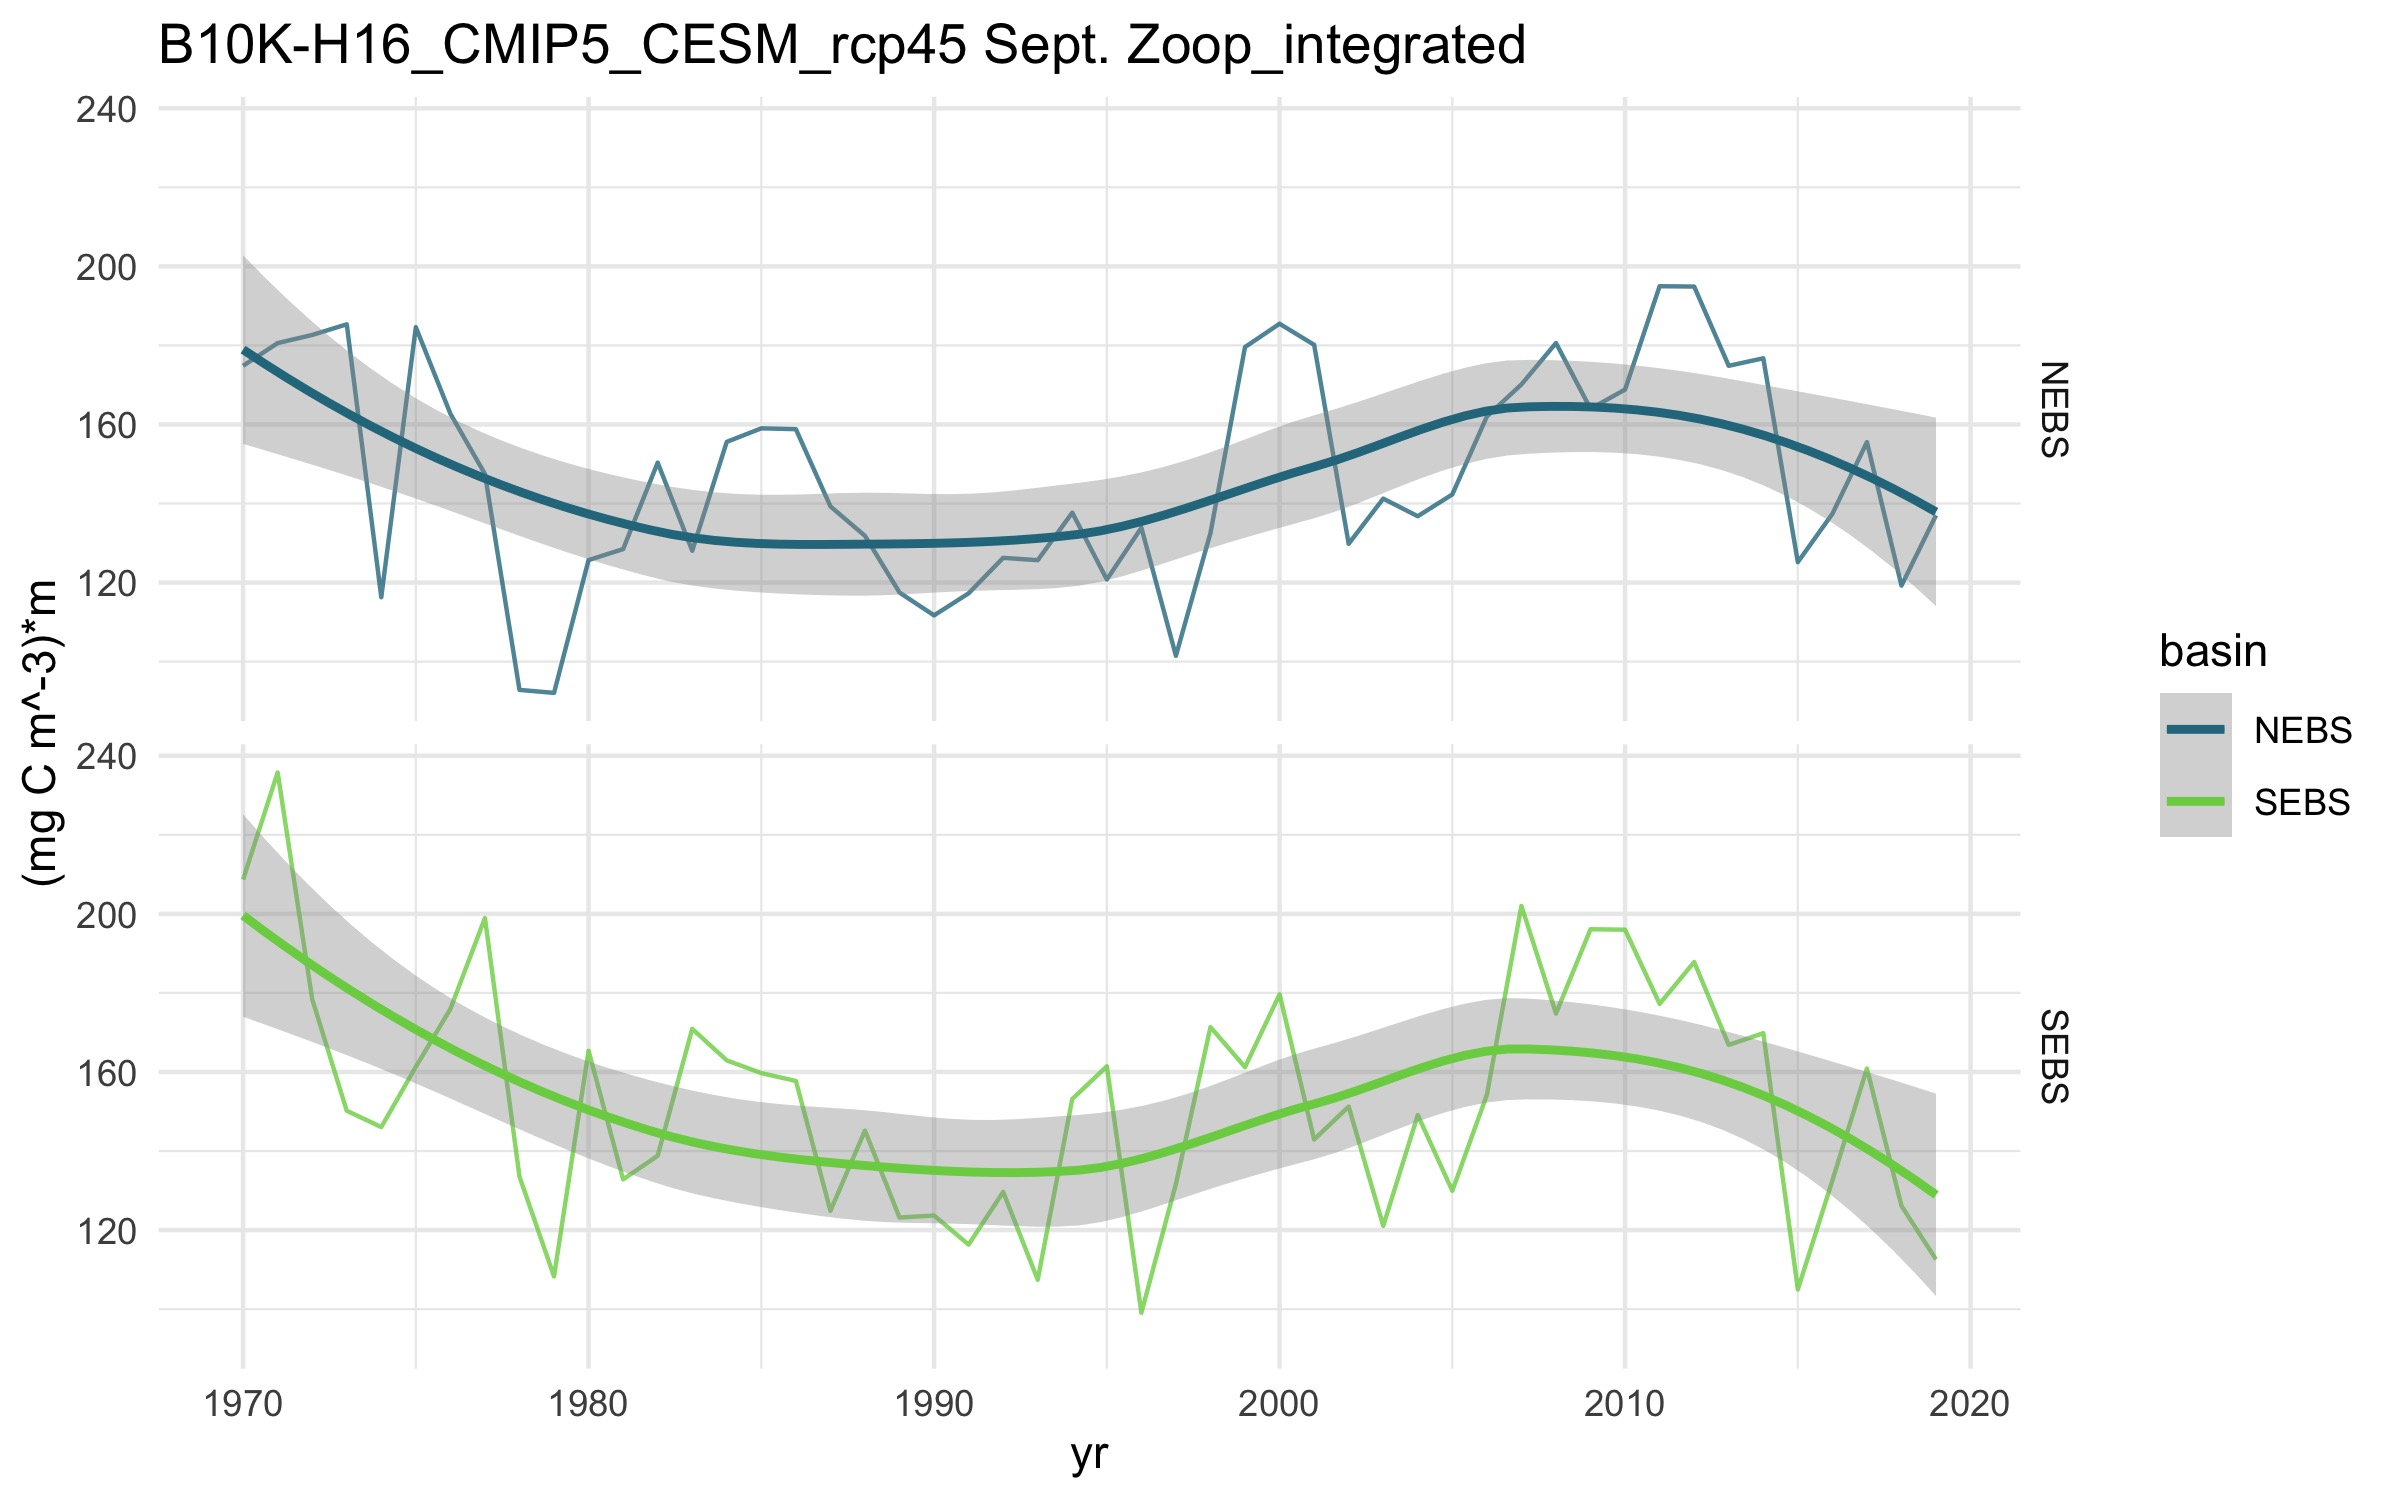
\includegraphics[width=0.75\textwidth,height=\textheight]{Figs/Hind_Sept_large_Zoop.jpg}
\caption{September large zooplankton integrated concentration}
\end{figure}

\hypertarget{misc}{%
\section{misc}\label{misc}}

\[B0^k_{input}= \bar{B0}^k_{(2004:2014)}\left(\frac{B0^{a}_{2015}}{\bar{B0}^a_{(2004:2014)}}\right) \]
Where B0kinput is the unfished biomass used for setting inputs of (e.g.,
B0ktarget = 0.4B0kinput) and is determined by re-scaling the spawning
stock biomass from the status quo assessment in 2015 (B0a2015) to the
average model spawning stock biomass for your model between 2004-2014
(i.e., B0k) using the average unfished biomass from the stock assessment
model during the same period (B0a).

\end{document}
